% Template KLTN cho SV trường ĐHKHTN
% Liên hệ: nqminh@fit.hcmus.edu.vn
% Last update: 08/06/2016

% Chú ý: đọc các phần chú ý đóng khung của file này và chỉnh lại cho phù hợp.
% Trước khi build, xóa hết các file được tạo ra trong quá trình build trước đó, và build theo thứ tự: BIB > PDF > PDF.
% Nếu cập nhật tài liệu tham khảo, cũng cần build lại theo cách trên.

\documentclass[oneside,a4paper,14pt]{extreport}

% Font tiếng Việt
\usepackage[T5]{fontenc}
\usepackage[utf8]{inputenc}
\DeclareTextSymbolDefault{\DH}{T1}

% Tài liệu tham khảo
\usepackage[
	sorting=nty,
	backend=bibtex,
	defernumbers=true]{biblatex}
\usepackage[unicode]{hyperref} % Bookmark tiếng Việt
\addbibresource{References/references.bib}

\makeatletter
\def\blx@maxline{77}
\makeatother

% Chèn hình, các hình trong luận văn được để trong thư mục Images/
\usepackage{graphicx}
\graphicspath{ {Images/} }

% Chèn và định dạng mã nguồn
\usepackage{listings}
\usepackage{color}
\definecolor{codegreen}{rgb}{0,0.6,0}
\definecolor{codegray}{rgb}{0.5,0.5,0.5}
\definecolor{codepurple}{rgb}{0.58,0,0.82}
\definecolor{backcolour}{rgb}{0.95,0.95,0.92}
\lstdefinestyle{mystyle}{
    backgroundcolor=\color{backcolour},   
    commentstyle=\color{codegreen},
    keywordstyle=\color{magenta},
    numberstyle=\tiny\color{codegray},
    stringstyle=\color{codepurple},
    basicstyle=\footnotesize,
    breakatwhitespace=false,         
    breaklines=true,                 
    captionpos=b,                    
    keepspaces=true,                 
    numbers=left,                    
    numbersep=5pt,                  
    showspaces=false,                
    showstringspaces=false,
    showtabs=false,                  
    tabsize=2
}
\lstset{style=mystyle}

% Chèn và định dạng mã giả
\usepackage{amsmath}
\usepackage{algorithm}
\usepackage[noend]{algpseudocode}
\makeatletter
\def\BState{\State\hskip-\ALG@thistlm}
\makeatother

% Bảng biểu
\usepackage{multirow}
\usepackage{array}
\newcolumntype{L}[1]{>{\raggedright\let\newline\\\arraybackslash\hspace{0pt}}m{#1}}
\newcolumntype{C}[1]{>{\centering\let\newline\\\arraybackslash\hspace{0pt}}m{#1}}
\newcolumntype{R}[1]{>{\raggedleft\let\newline\\\arraybackslash\hspace{0pt}}m{#1}}

% Đổi tên mặc định
\renewcommand{\chaptername}{Chương}
\renewcommand{\figurename}{Hình}
\renewcommand{\tablename}{Bảng}
\renewcommand{\contentsname}{Mục lục}
\renewcommand{\listfigurename}{Danh sách hình}
\renewcommand{\listtablename}{Danh sách bảng}
\renewcommand{\appendixname}{Phụ lục}

% Dãn dòng 1.5
\usepackage{setspace}
\onehalfspacing

% Thụt vào đầu dòng
\usepackage{indentfirst}

% Canh lề
\usepackage[
  top=30mm,
  bottom=25mm,
  left=30mm,
  right=20mm,
  includefoot]{geometry}
  
% Trang bìa
\usepackage{tikz}
\usetikzlibrary{calc}
\newcommand\HRule{\rule{\textwidth}{1pt}}

% ========================================================================================= %
% CHÚ Ý: Thông tin chung về KLTN - sinh viên điền vào đây để tự động update các trang khác  %
% ========================================================================================= %
\newcommand{\tenSV}{Nguyễn~Ngọc~Lan~Như~-~Hoàng~Minh~Quân} % Dấu ~ là khoảng trắng không được tách (các chữ nối với nhau bằng dấu ~ sẽ nằm cùng 1 dòng
\newcommand{\mssv}{1234567}
\newcommand{\tenKL}{Sử~dụng~LaTeX trong Khoá~luận~tốt~nghiệp} % Chú ý dấu ~ trong tên khóa luận
\newcommand{\tenGVHD}{Tên~Giáo~Viên}
\newcommand{\tenBM}{Công nghệ tri thức}

\begin{document}

\begin{titlepage}

\begin{center}
%ĐẠI HỌC QUỐC GIA THÀNH PHỐ HỒ CHÍ MINH\\
TRƯỜNG ĐẠI HỌC KHOA HỌC TỰ NHIÊN\\
\textbf{KHOA CÔNG NGHỆ THÔNG TIN}\\[2cm]


{ \Large \bfseries Nguyễn Ngọc Lan Như - Hoàng Minh Quân\\[2cm] } 

%Tên đề tài Khóa luận tốt nghiệp/Đồ án tốt nghiệp

{ \Large \bfseries HUẤN LUYỆN \\MẠNG NƠ-RON NHIỀU TẦNG ẨN \\BẰNG THUẬT TOÁN ADAM \\[3cm]} 


%Chọn trong các dòng sau
\large KHÓA LUẬN TỐT NGHIỆP CỬ NHÂN\\
%\large ĐỒ ÁN TỐT NGHIỆP CỬ NHÂN\\
%\large THỰC TẬP TỐT NGHIỆP CỬ NHÂN\\
%Đưa vào dòng này nếu thuộc chương trình Chất lượng cao, hoặc lớp Cử nhân tài năng
\large CHƯƠNG TRÌNH CHÍNH QUY\\
%\large CHƯƠNG TRÌNH CHẤT LƯỢNG CAO\\
%\large CHƯƠNG TRÌNH CỬ NHÂN TÀI NĂNG\\[2cm]


\begin{tikzpicture}[remember picture, overlay]
  \draw[line width = 2pt] ($(current page.north west) + (2cm,-2cm)$) rectangle ($(current page.south east) + (-1.5cm,2cm)$);
\end{tikzpicture}

\vfill
Tp. Hồ Chí Minh, tháng 07/2021

\end{center}

\pagebreak



\begin{center}

TRƯỜNG ĐẠI HỌC KHOA HỌC TỰ NHIÊN\\
\textbf{KHOA CÔNG NGHỆ THÔNG TIN}\\[2cm]


{\large \bfseries Nguyễn Ngọc Lan Như - 1712644\\} 
{\large \bfseries Hoàng Minh Quân - 1712688\\[2cm]}

%Tên đề tài Khóa luận tốt nghiệp/Đồ án tốt nghiệp

{ \Large \bfseries HUẤN LUYỆN \\MẠNG NƠ-RON NHIỀU TẦNG ẨN \\BẰNG THUẬT TOÁN ADAM \\[2cm] } 


%Chọn trong các dòng sau
\large KHÓA LUẬN TỐT NGHIỆP CỬ NHÂN\\
%\large ĐỒ ÁN TỐT NGHIỆP CỬ NHÂN\\
%Đưa vào dòng này nếu thuộc chương trình Chất lượng cao, hoặc lớp Cử nhân tài năng
\large CHƯƠNG TRÌNH CHÍNH QUY\\[2cm]
%\large CHƯƠNG TRÌNH CHẤT LƯỢNG CAO\\[2cm]
%\large CHƯƠNG TRÌNH CỬ NHÂN TÀI NĂNG\\[2cm]

\textbf{GIÁO VIÊN HƯỚNG DẪN}\\
ThS. Trần Trung Kiên

\begin{tikzpicture}[remember picture, overlay]
  \draw[line width = 2pt] ($(current page.north west) + (2cm,-2cm)$) rectangle ($(current page.south east) + (-1.5cm,2cm)$);
\end{tikzpicture}

\vfill
Tp. Hồ Chí Minh, tháng 07/2021

\end{center}

\end{titlepage}
% Sasu trang Title, các bạn chèn nhận xét gủa GVHD và GVPB. Nhận xét sẽ được giáo vụ phát sau buổi bảo vệ để các bạn đóng quyển.

\pagenumbering{roman} % Đánh số i, ii, iii, ...

%\addcontentsline{toc}{chapter}{Lời cam đoan}
%\chapter*{Lời cam đoan}
\label{reassurances}

Tôi xin cam đoan đây là công trình nghiên cứu của riêng tôi. Các số liệu và kết quả nghiên cứu trong luận văn này là trung thực và không trùng lặp với các đề tài khác.

\addcontentsline{toc}{chapter}{Lời cảm ơn}
\chapter*{Lời cảm ơn}
\label{thanks}

Đầu tiên, chúng em xin chân thành cảm ơn Thầy Trần Trung Kiên vì đã đồng hành cùng chúng em trong suốt quá trình thực hiện khóa luận này. Từ khi mới bắt đầu chọn những đề tài đầu tiên, cho đến những công đoạn cuối cùng để chuẩn bị báo cáo, Thầy vẫn luôn rất tận tâm và nhiệt tình hướng dẫn chúng em trong tất cả các vấn đề, khúc mắc mà chúng em gặp phải. Chúng em cảm thấy thật sự may mắn khi được học tập và làm việc với Thầy từ môn Nhập môn học máy vào Học kì 5, cho đến khóa luận này để kết thúc chặng đường sinh viên.

Chúng em xin cảm ơn quý Thầy Cô khoa Công Nghệ Thông Tin - trường Đại học Khoa Học Tự Nhiên đã truyền đạt cho chúng em những kiến thức quý báu trong suốt 4 năm học tập tại trường. Những kiến thức này sẽ là hành trang không thể thiếu cho những chặng đường trong tương lai mà chúng em theo đuổi.

Chúng con xin cảm ơn công ơn sinh thành và dưỡng dục của ba mẹ để chúng con có được thành quả như ngày hôm nay. Tình yêu thương vô điều kiện và sự hy sinh thầm lặng của ba mẹ sẽ luôn là lý do giúp chúng con vượt qua những đoạn đường khó khăn trong cuộc sống.

\hfill Tp. Hồ Chí Minh, 06/2021

\hfill \textit{Người thực hiện}

\hfill \textit{Nguyễn Ngọc Lan Như - Hoàng Minh Quân}

%\addcontentsline{toc}{chapter}{Đề cương chi tiết}
%\include{Appendix/decuong}

% Mục lục, danh sách hình, danh sách bảng
\newpage
\renewcommand{\contentsname}{\centerline{Mục lục}}
\addcontentsline{toc}{chapter}{Mục lục}
\tableofcontents

\newpage
\renewcommand\listfigurename{\centerline{Danh mục hình ảnh}}
\addcontentsline{toc}{chapter}{Danh mục hình ảnh}
\listoffigures

\newpage
\renewcommand\listtablename{\centerline{Danh mục bảng}}
\addcontentsline{toc}{chapter}{Danh mục bảng}
\listoftables

%\addcontentsline{toc}{chapter}{Tóm tắt}
%\chapter*{Tóm tắt}
\label{summary}

Trong nhiều năm trở lại đây, các mô hình mạng nơ-ron nhiều tầng ẩn đã tạo nên những bước cải tiến lớn trong vô số lĩnh vực khoa học khác nhau. Để đạt được những kết quả đó, tất cả mô hình đều yêu cầu một quá trình điều chỉnh bộ trọng số để mô hình có thể thích ứng với dữ liệu huấn luyện và dự đoán trên dữ liệu mới một cách chính xác. Vì vậy, một phương pháp đi tìm bộ trọng số hiệu quả sẽ cải thiện độ chính xác của mô hình, rút ngắn thời gian huấn luyện, từ đó nâng cao tính ứng dụng của các mô hình mạng nơ-ron nhiều tầng ẩn.

Khóa luận tập trung tìm hiểu về những khó khăn trong việc huấn luyện mạng nơ-ron nhiều tầng ẩn và cách mà các thuật toán tối ưu giải quyết những khó khăn đó, với trọng tâm là thuật toán Adam. Thuật toán Adam được giới thiệu trong bài báo ``Adam: A Method for Stochastic Optimization'' công bố tại hội nghị ``International Conference on Learning Representation 2015''. Ý tưởng của thuật toán là kết hợp hai hướng tiếp cận: (1) sử dụng quán tính để tăng tốc và giảm dao động, và (2) thích ứng lượng cập nhật cho từng trọng số; với mục tiêu kế thừa được những điểm mạnh và đồng thời cải thiện những điểm yếu của mỗi hướng tiếp cận.

Kết quả đạt được của khóa luận là cài đặt lại thuật toán Adam cùng các thuật toán liên quan và tái tạo được một phần kết quả bài báo gốc. Khóa luận cũng thực hiện thêm các thí nghiệm nhằm phân tích và làm rõ cách mỗi phương pháp giải quyết các khó khăn trong việc huấn luyện mạng nơ-ron nhiều tầng ẩn.

\clearpage

\pagenumbering{arabic} % Đánh số 1, 2, 3, ...

% Các chương nội dung
\chapter{Giới thiệu}
\label{Chapter1}

Các mạng nơ-ron nhiều tầng ẩn có tính ứng dụng cao và ảnh hưởng lớn tới ngành trí tuệ nhân tạo. Đầu tiên, các bài toán khó đối với máy tính như xử lý ảnh và ngôn ngữ tự nhiên đã phần nào được giải quyết. Thứ hai, các mô hình mạng nơ-ron có thể được sử dụng trong nhiều bài toán khác nhau, từ đó tăng tính ứng dụng vào thực tế. Thứ ba, các lý thuyết liên quan đến mạng nơ-ron nhiều tầng ẩn vẫn còn nhiều câu hỏi chưa có lời giải đáp, cho thấy tiềm năng của hướng phát triển này.

Mạng nơ-ron nhân tạo (Artificial Neural Network) gồm: tầng nhập, các tầng ẩn và tầng xuất. Mỗi tầng được cấu thành từ nhiều đơn vị tính toán mà ta gọi là các nơ-ron. Các nơ-ron được liên kết với nơ-ron ở tầng tiếp theo bằng các liên kết có trọng số đại diện cho mức độ quan trọng của tín hiệu từ nơ-ron này sang nơ-ron khác. Số lượng trọng số sẽ tăng theo số lượng tầng ẩn có trong mạng cũng như số lượng nơ-ron của mỗi tầng ẩn. Mạng nơ-ron nhân tạo có hơn một tầng ẩn được gọi là mạng nơ-ron nhiều tầng ẩn, hay mạng nơ-ron sâu (Deep Neural Network); ngược lại, gọi là mạng nơ-ron có ít tầng ẩn, hay mạng nơ-ron nông (Shallow Neural Network). Việc có nhiều tầng ẩn giúp mạng biểu diễn được các hàm phức tạp mà các mô hình học máy truyền thống không biểu diễn được. Ngoài ra, mạng học sâu còn có thể biểu diễn được cùng một tập hàm nhưng với số lượng trọng số ít hơn mạng nơ-ron nông \cite{bengio2009learning}. Sức mạnh rút trích đặc trưng tự động của mạng nơ-ron nhiều tầng ẩn đã được chỉ ra trong nhiều bài báo khác: Yoshua Bengio và Yann LeCun lý giải rằng với nhiều tầng ẩn, mạng nơ-ron có thể ``học'' được từ đặc trưng đơn giản (low-level features) và tạo thành các đặc trưng phức tạp hơn (higher-level features) (hình \ref{fig:layers-features}) \cite{bengio2007scaling}.

\begin{figure}[htp]
	\centering
	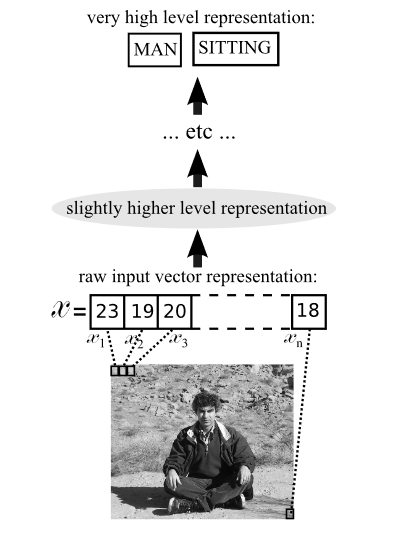
\includegraphics[width=115 mm]{images/layers-features.png}
	\caption{Minh hoạ quá trình mạng nơ-ron ``học'' từ các đặc trưng đơn giản, như các điểm ảnh, tạo thành các đặc trưng phức tạp hơn \cite{bengio2009learning}.}
	\label{fig:layers-features}
\end{figure}

Tuy nhiên, mặc dù mạng nơ-ron có càng nhiều tầng ẩn sẽ khiến cho độ chính xác trong tập huấn luyện ngày càng tăng nhưng có thể làm cho độ chính xác trong tập kiểm thử ngày càng giảm. Đây là biểu hiện của việc mô hình bị ``overfit'', đồng nghĩa với việc mô hình chỉ ``ghi nhớ'' tập huấn luyện nhưng không thể tổng quát hóa những đặc trưng đã học để tiến hành đưa ra dự đoán trên tập kiểm thử. Ngược lại, nếu mạng nơ-ron quá đơn giản, có thể có ít tầng ẩn hoặc mỗi tầng ẩn có số lượng nơ-ron ít, thì mô hình đó không đủ khả năng để rút trích ra những đặc trưng có ý nghĩa dự đoán khiến cho độ chính xác ở cả hai tập dữ liệu huấn luyện và kiểm thử đều giảm (hình \ref{fig:under-over}).

\begin{figure}[htp]
	\centering
	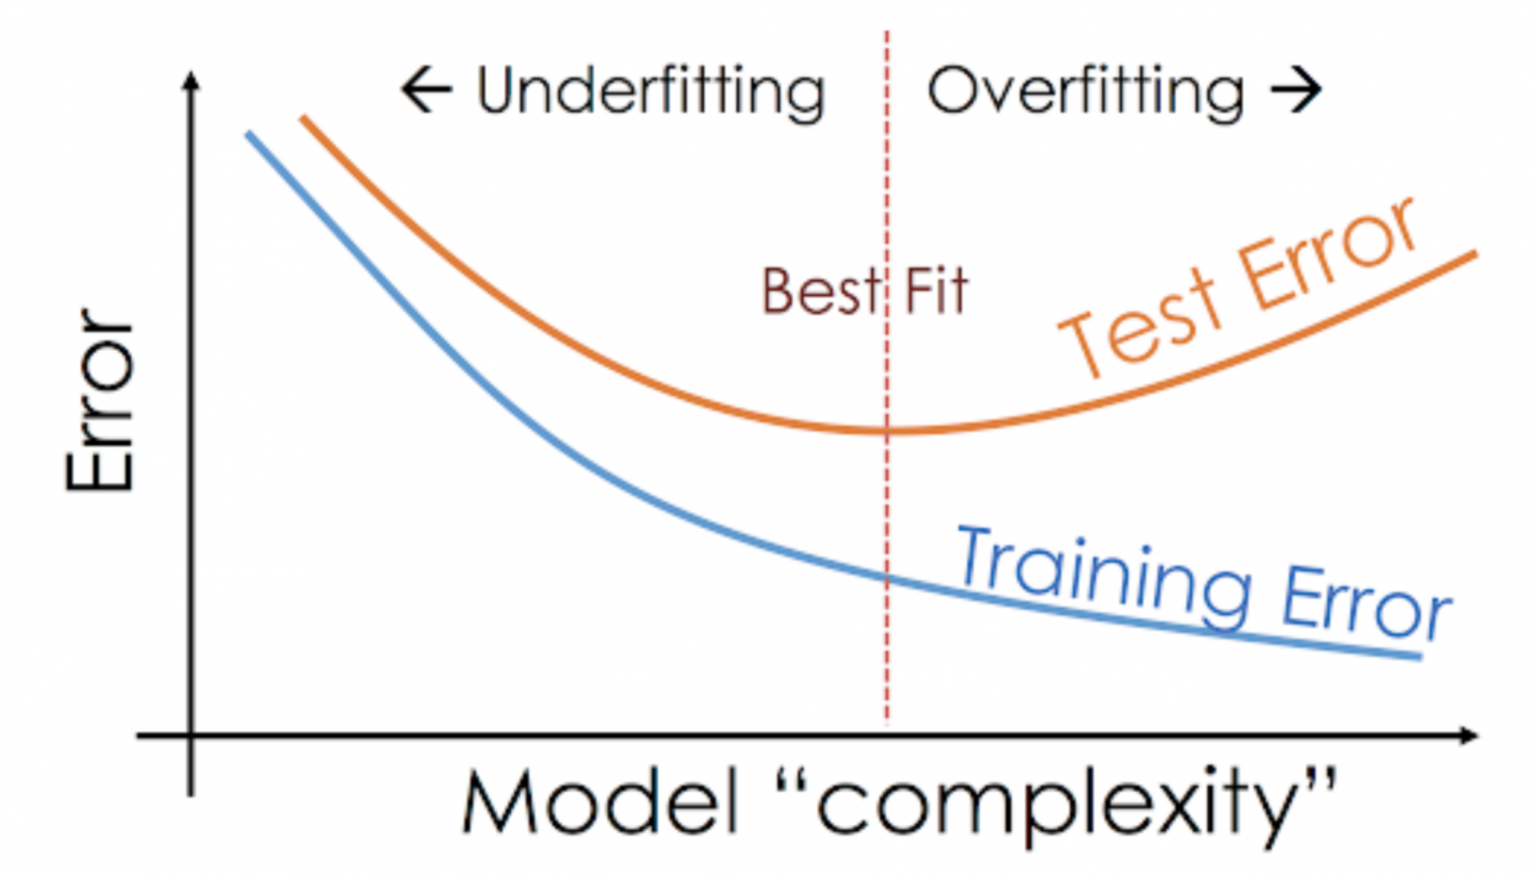
\includegraphics[width=100 mm]{images/under-over.png}
	\caption{Minh họa cho mô hình overfit và underfit. (Nguồn: \url{https://www.analyticsvidhya.com/blog/2020/02/underfitting-overfitting-best-fitting-machine-learning})}
	\label{fig:under-over}
\end{figure}

Một mạng nơ-ron nhiều tầng ẩn được xem là có khả năng tổng quát hoá tốt trên một bài toán khi sự sai khác giữa giá trị dự đoán của mạng nơ-ron và giá trị nhãn của dữ liệu ngoài tập huấn luyện là đủ nhỏ (trong bài toán huấn luyện có giám sát). Để đạt được kết quả đó, mạng nơ-ron nhiều tầng ẩn cần đi tìm một bộ trọng số phù hợp cho từng bài toán cụ thể. Việc đi tìm bộ trọng số này được thực hiện thông qua quá trình huấn luyện mạng nơ-ron nhiều tầng ẩn.

Bài toán huấn luyện mạng nơ-ron nhiều tầng ẩn nhận dữ liệu nhập là hàm chi phí nhận bộ trọng số của mạng nơ-ron nhiều tầng ẩn làm tham số. Hàm chi phí cho biết sự sai lệch giữa kết quả dự đoán của mạng nơ-ron so với giá trị đúng. Giá trị sai lệch này còn được gọi là độ lỗi. Sau quá trình huấn luyện, ta mong muốn có được một bộ trọng số của mạng nơ-ron nhiều tầng ẩn cho độ lỗi trong cả hai tập dữ liệu huấn luyện và tập dữ liệu kiểm thử là đủ nhỏ.

\begin{figure}[htp]
	\centering
	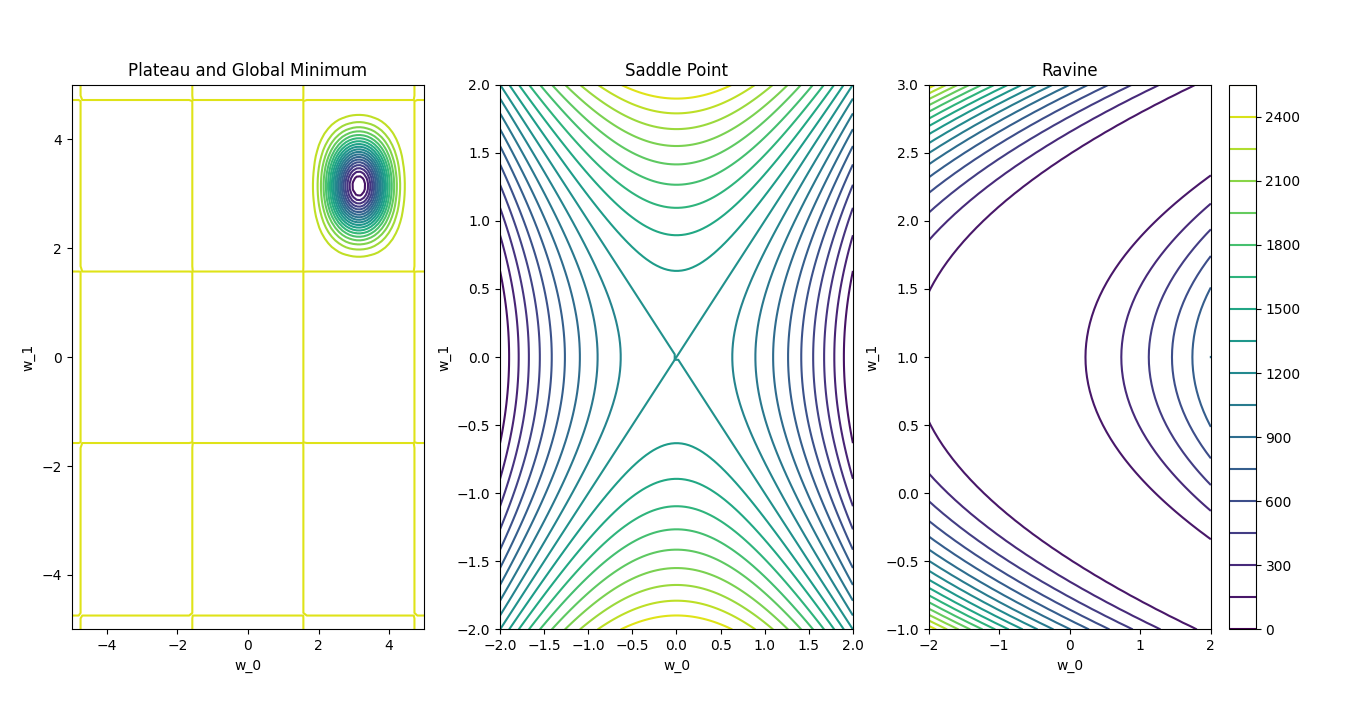
\includegraphics[width=120 mm]{images/cricial-point-contour.png}
	\caption{Đồ thị contour cho những điểm critical point: vùng bằng phẳng có một cực tiểu (trái), điểm yên ngựa (giữa), vùng rãnh hẹp (phải).}
	\label{fig:cricial-point-contour}
\end{figure}

Việc huấn luyện, hay tối ưu hoá mạng nơ-ron có thể hiểu là quá trình đi tìm cực tiểu của hàm chi phí bằng cách thay đổi giá trị của bộ trọng số. Từ đó, ta cũng có thể hiểu quá trình tối ưu hóa mạng nơ-ron là quá trình di chuyển trong bề mặt lỗi (hình \ref{fig:resnet-loss}) dựa trên hướng của véc-tơ đạo hàm riêng, còn được gọi là gradient. Tuy nhiên, việc di chuyển trong bề mặt lỗi gặp nhiều khó khăn. Li Hao và cộng sự \cite{li2018visualizing} cho thấy rằng sự phức tạp của bề mặt lỗi ngày càng tăng khi số tầng ẩn trọng mạng nơ-ron ngày càng tăng. Sự hỗn loạn này được cấu thành từ nhiều ``critical point'' (``critical point'' là những điểm có gradient bằng 0 như cực tiểu địa phương, điểm yên ngựa) hợp với các vùng bằng phẳng, và vùng rãnh hẹp (hình \ref{fig:cricial-point-contour}).

\begin{figure}[htp]
	\centering
	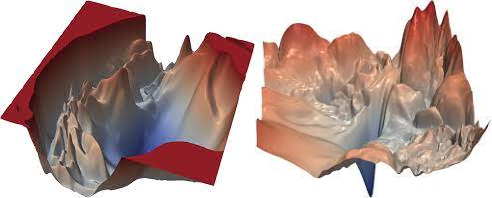
\includegraphics[width=120 mm]{images/resnet-loss.png}
	\caption{Bề mặt lỗi của mô hình ResNet-110 (trái) và bề mặt lỗi của mô hình ResNet-56 (phải) \cite{li2018visualizing}.}
	\label{fig:resnet-loss}
\end{figure}

Các điểm cực tiểu địa phương từng được xem như là nguyên nhân chính gây ra sự khó khăn trong việc tối ưu hoá mạng nơ-ron có nhiều tầng ẩn, nhưng nghiên cứu của Quynh Nguyen và Matthias Hein \cite{nguyen2017thelosssurface} đã chỉ ra rằng việc đi tìm cực tiểu toàn cục có thể mất nhiều thời gian nhưng cho hiệu quả không đáng kể. Yann N. Dauphin cũng cho rằng khi số lượng tầng ẩn quá lớn thì phần lớn các điểm critical point sẽ là điểm yên ngựa, và các điểm cực tiểu tìm được đều có độ lỗi ngang với cực tiểu toàn cục. Hơn nữa, các điểm yên ngựa thường được bao bọc bởi một vùng gần như bằng phẳng, là vùng mà tại đó đạo hàm gần bằng 0, làm chậm tốc độ của đa số các thuật toán tối ưu thường được sử dụng hiện nay.

\begin{figure}[htp]
	\centering
	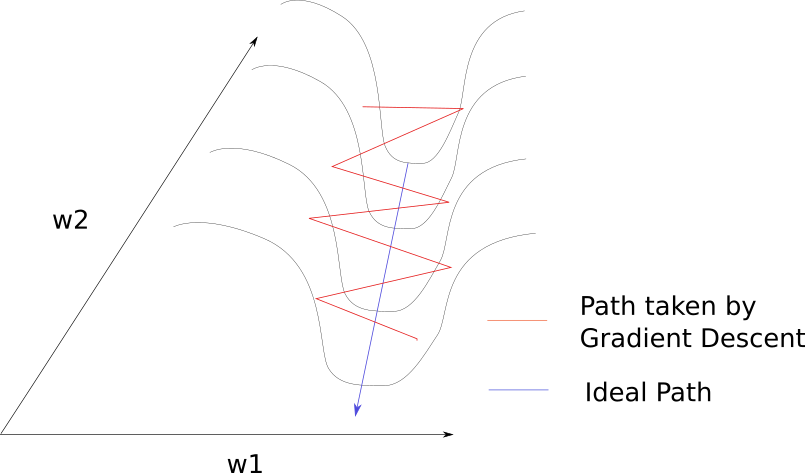
\includegraphics[width=100 mm]{images/valley.png}
	\caption{Minh họa cho hướng đi của gradient trong trường hợp di chuyển trong rãnh hẹp. (Nguồn: \url{https://blog.paperspace.com/intro-to-optimization-momentum-rmsprop-adam/})}
	\label{fig:valley}
\end{figure}

Ngoài các điểm yên ngựa, bề mặt lỗi còn đặc trưng bởi độ cong tại mỗi hướng tương ứng với một trọng số của mạng nơ-ron nhiều tầng ẩn. Một hướng có độ cong thấp (low-curvature, như hướng $w_2$ trong hình \ref{fig:valley}) đồng nghĩa với gradient sẽ ít thay đổi và ngược lại, một hướng có độ cong cao (high-curvature, như hướng $w_1$ trong hình \ref{fig:valley}) sẽ có gradient thay đổi nhiều. Vùng được đồng thời tạo bởi các hướng có độ cong cao và độ cong thấp được gọi là vùng rãnh hẹp. Các vùng này được tạo ra do ảnh hưởng của các trọng số $w_1$ và $w_2$ lên độ lỗi là không giống nhau. Một $w_1$ có giá trị gấp 10 lần giá trị của $w_2$ sẽ cho tín hiệu của các nơ-ron được liên kết bằng $w_1$ ảnh hưởng lên độ lỗi gấp 10 lần tín hiệu của các nơ-ron được liên kết bằng $w_2$, dẫn đến độ cong theo hướng $w_1$ sẽ cao hơn độ cong theo hướng $w_2$ gấp 10 lần. Sự cách biệt lớn trong độ lớn của các giá trị trọng số này tạo ra vùng rãnh hẹp. Hiện tượng này thường xuyên xảy ra trong mạng nơ-ron do tín hiệu của các nơ-ron khác nhau có mức độ ảnh hưởng khác nhau đến quá trình dự đoán, và càng nghiêm trọng hơn trong các mạng nơ-ron nhiều tầng ẩn.

Phương pháp đầu tiên được dùng trong huấn luyện mạng nơ-ron thực hiện bước từng bước nhỏ từ một điểm bất kỳ theo hướng ngược lại với hướng có độ tăng lớn nhất, hướng của véc-tơ đạo hàm riêng gradient, tìm đến điểm cho độ lỗi nhỏ hơn được gọi là ``Gradient Descent'' (GD). Tuy nhiên, phương pháp này tốn nhiều thời gian tính toán véc-tơ gradient tại điểm hiện tại. Các đạo hàm riêng theo từng trọng số trong gradient có được từ việc lấy đạo hàm của trung bình độ lỗi trên toàn bộ điểm dữ liệu. Với kích thước tập dữ liệu cần cho huấn luyện mạng nơ-ron nhiều tầng ẩn càng lớn thì việc tính toán gradient tại mỗi bước lại càng mất nhiều thời gian. Để cải thiện vấn đề này, một phương pháp khác không sử dụng toàn bộ điểm dữ liệu để thực hiện một bước cập nhật, thay vào đó, chỉ một tập con lấy ngẫu nhiên được sử dụng để tính véc-tơ gradient tại mỗi bước. Phương pháp này được gọi là ``Stochastic Gradient Descent'' (SGD). Vì thực hiện tính toán trên một tập con dữ liệu nên hướng gradient của SGD chỉ là một xấp xỉ của hướng gradient thật của bề mặt lỗi có độ sai số tỉ lệ nghịch với kích thước tập con.

Tuy nhiên, SGD thực hiện một bước nhảy tỉ lệ với độ lớn của gradient nên gặp khó khăn khi di chuyển trong các vùng rãnh hẹp và vùng có độ nghiêng nhỏ. Trong những vùng này, ta mong muốn độ lớn bước cập nhật tỉ lệ nghịch với độ lớn của gradient. Vì vùng có độ lớn gradient nhỏ thì một bước đi dài sẽ giúp giảm thời gian di chuyển trong khi những vùng có gradient lớn cần bước những bước nhỏ hơn. Sự điều chỉnh này trong bước cập nhật của SGD cho ta thuật toán ``SGD với Momentum'', hay ``Momentum''. Thuật toán Momentum cập nhật trọng số dựa trên gradient của bước hiện tại và gradient của những bước cập nhật gần nhất. Từ đó, một lượng ``quán tính" được thêm vào giúp triệt tiêu các hướng có độ cong cao và cho phép một bước cập nhật lớn hơn tại hướng có độ dốc thấp. Bước cải tiến này không chỉ giúp thuật toán Momentum thực hiện những bước cập nhật có ý nghĩa trong vùng rãnh hẹp và vùng có độ nghiêng nhỏ mà còn giúp xấp xỉ gradient trong SGD gần hơn với gradient thật của bề mặt lỗi từ đó tăng độ chính xác trong hướng di chuyển của thuật toán.

Thuật toán SGD với Momentum giúp cải thiện tốc độ huấn luyện mạng nơ-ron đáng kể và vẫn được sử dụng trong một số mạng nơ-ron nhiều tầng ẩn hiện nay. Mặc dù vậy thuật toán vẫn chưa giải quyết được các khó khăn vì lượng "quán tính" được thêm vào không có nhiều hiệu quả trong những vùng rãnh hẹp mà độ lớn của đạo hàm riêng tại mỗi hướng cập nhật rất khác nhau. Richard S. Sutton cho rằng để có được một bước cập nhật có hiệu quả thì tỉ lệ học cần phải được thay đổi ứng với độ cong của từng hướng\cite{sutton1986two}. Đây là một trong những lý do các phương pháp bậc hai được sử dụng. Các phương pháp bậc hai là những phương pháp sử dụng ma trận Hessian — là ma trận đạo hàm riêng bậc hai theo từng cặp hướng — để ước lượng độ cong tại một điểm trên bề mặt lỗi. Từ các ước lượng bậc hai này mà các phương pháp bậc hai cho bước cập nhật tốt hơn các phương pháp chỉ sử dụng gradient.

Mặc dù phương pháp bậc hai cho các bước cập nhật tối ưu nhưng có hai nguyên nhân dẫn tới các phương pháp này ít được sử dụng trong huấn luyện mạng nơ-ron nhiều tầng ẩn hiện nay. Đầu tiên, việc sử dụng các xấp xỉ bậc hai dẫn đến dao động tại vùng gần cực tiểu kéo dài thời gian huấn luyện và có khả năng không thể hội tụ. Khó khăn thứ hai đến từ việc tính toán ma trận Hessian đòi hỏi nhiều chi phí tính toán và tiêu tốn bộ nhớ cấp số mũ với số lượng trọng số của mạng. Đối với các mạng nơ-ron nhiều tầng ẩn có số trọng số có thể lên tới hàng tỷ thì đây là điều bất khả thi. Vì vậy, một số phương pháp bậc nhất thực hiện xấp xỉ ma trận Hessian thông qua gradient bậc nhất. Đây là ý tưởng chính của các thuật toán sử dụng tỉ lệ học thích ứng. Các thuật toán này điều chỉnh tỉ lệ học tại từng hường bằng cách sử dụng bình phương đạo hàm riêng bậc nhất của trọng số tương ứng. Vì mỗi trọng số được cập nhật một lượng riêng lẻ nên véc-tơ đạo hàm riêng là một hình chiếu của véc-tơ gradient trên trục trọng số tương ứng. Độ dài của véc-tơ hình chiếu sẽ lớn nhất khi véc-tơ gradient song song với trục và giảm dần khi véc-tơ gradient càng vuông góc với trục. Chính vì lý do đó mà các thuật toán sử dụng tỉ lệ học thích ứng gặp nhiều khó khăn khi các hướng tối ưu không phải là hướng song song với trục trọng số.

Lấy ý tưởng từ những phương pháp trên, Diederik P. Kingma và Jimmy Lei Ba đã đề xuất một thuật toán tối ưu bậc nhất cho mạng nơ-ron nhiều tầng ẩn với tốc độ cao hơn so với hầu hết những thuật toán trước đó \cite{kingma2014adam}. Công trình này, ``Adam, A Method for Stochastic Optimization'', được công bố tại hội nghị ``International Conference on Learning Representation 2015''. Ý tưởng của thuật toán là kết hợp hai hướng tiếp cận trước đó: (1) sử dụng quán tính để tăng tốc và giảm dao động, và (2) thích ứng tỉ lệ học cho từng trọng số. Thuật toán Adam sử dụng trung bình chạy để tích tụ quán tính kết hợp với phương pháp xấp xỉ ma trận Hessian của phương pháp tỉ lệ học thích ứng. Sự kết hợp này cho phép thực hiện các bước cập nhật tốt hơn tại vùng có độ lớn đạo hàm riêng trên mỗi hướng rất khác nhau. Đồng thời cũng cải thiện độ lớn của bước cập nhật khi véc-tơ gradient không song song với trục trọng số. Ngoài ra, Adam còn thực hiện ``bias-correction'' giúp thuật toán không bị ``bias'' về giá trị khởi tạo cho phép thực hiện các bước cập nhật tốt hơn ngay những bước đầu tiên. Trong khóa luận này, chúng tôi tìm hiểu và cài đặt lại thuật toán Adam cùng với các thuật toán liên quan. Chúng tôi cũng thực hiện thêm các thí nghiệm nhằm phân tích và làm rõ cách mỗi phương pháp giải quyết các khó khăn trong việc huấn luyện mạng nơ-ron nhiều tầng ẩn. Ngoài ra, chúng tôi cũng sử dụng tính toán song song trên GPU để tăng tốc độ xử lí cho các thí nghiệm.

Phần còn lại của khóa luận được trình bày như sau:

\begin{itemize}
	\item Chương 2 giới thiệu sơ lược về mạng nơ-ron nhiều tầng ẩn và quá trình huấn luyện, cũng như nguyên lý của thuật toán Gradient Descent.
	\item Chương 3 trình bày về thuật toán Adam và các thuật toán nền tảng. Chương này là phần chính của khóa luận.
	\item Chương 4 trình bày về các thí nghiệm về nguyên lý cũng như thực tiễn để phân tích các tính chất của thuật toán Adam.
	\item Cuối cùng, chương 5 trình bày kết luận và hướng phát triển.
\end{itemize}


\chapter{Kiến thức nền tảng}
\label{Chapter2}

\textit{Trong chương này, chúng tôi trình bày các kiến thức nền tảng được sử dụng trong khóa luận. Đầu tiên, chúng tôi trình bày động lực phát triển và kiến trúc của một mạng nơ-ron nhiều tầng ẩn. Sau đó, chúng tôi tiếp tục giới thiệu những khó khăn của bài toán tối ưu cần được giải quyết khi huấn luyện mạng nơ-ron nhiều tầng ẩn. Tiếp theo, chúng tôi trình bày về thuật toán tối ưu cơ bản là Gradient Descent (GD) và phiên bản cải tiến là Stochastic Gradient Descent (SGD) để có thể giúp tối ưu hóa nhanh hơn khi tập dữ liệu huấn luyện có kích thước lớn. GD/SGD sẽ là nền tảng cho các thuật toán tối ưu hóa được trình bày ở chương \ref{Chapter3}. Cuối cùng, chúng tôi trình bày về thuật toán lan truyền ngược (backpropagation) để tính véc-tơ đạo hàm riêng của độ lỗi theo từng trọng số của mạng nơ-ron nhiều tầng ẩn.}

\section{Mạng nơ-ron nhiều tầng ẩn}

Ngay từ những ngày đầu tiên của điện toán, những nhà khoa học đã hướng đến việc tạo ra những chiếc máy tính có thể thực hiện các tác vụ đòi hỏi khả năng suy nghĩ như bộ não con người. Mục tiêu cuối cùng của những chiếc máy tính này là thay thế con người thực hiện các tác vụ phức tạp như nhận diện vật thể trong hình ảnh, hiểu được ý nghĩa của ngôn ngữ tự nhiên, cũng như chơi được những trò chơi trí tuệ như cờ vua và cờ vây. Hướng nghiên cứu những phương pháp cung cấp cho máy tính khả năng suy nghĩ như con người được gọi là ``trí tuệ nhân tạo'' (artificial intelligence).

Các phương pháp trí tuệ nhân tạo truyền thống có thể giải quyết được một số bài toán như tìm đường đi tối ưu một cách nhanh hơn, giải một số trò chơi như 8-puzzle, và thậm chí có thể đánh cờ vua ở trình độ Grandmaster (Đại kiện tướng) \cite{campbell2001deepblue}. Tuy nhiên, những phương pháp này chưa đủ sức giải quyết các bài toán cấp cao như nhận diện thông tin trong ảnh và văn bản. Lí do là vì trí tuệ nhân tạo truyền thống cần các đặc trưng thủ công (hand-crafted features) dựa trên những hiểu biết của con người về dữ liệu và bài toán đó. Một nhánh nghiên cứu hướng tới máy tính có thể rút trích những đặc trưng đó một cách tự động thông qua việc huấn luyện một mô hình thích ứng với dữ liệu được gọi là học máy (machine learning). Các mô hình học máy cho phép máy tính có thể chuyển đổi các đặc trưng đơn giản ban đầu thành ``kiến thức'' để hỗ trợ trong việc dự đoán. Nhờ có những ``kiến thức'' này mà các mô hình máy học có thể được ứng dụng trong nhiều lĩnh vực khác nhau.

\begin{figure}[htp]
	\centering
	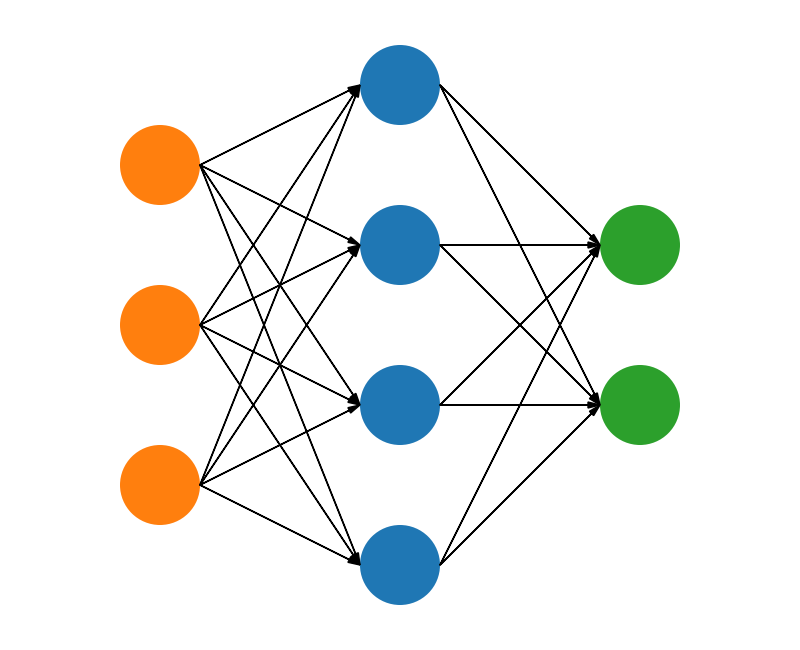
\includegraphics[width=80 mm]{images/ann.png}
	\caption{Mô hình mạng nơ-ron nhân tạo với tầng nhập (màu cam), tầng ẩn (màu xanh dương) và tầng xuất (màu xanh lá).}
	\label{fig:ann}
\end{figure}

Trong những phương pháp học máy được phát triển, nhóm phương pháp ``mạng nơ-ron nhân tạo'' (artificial neural network) (hình \ref{fig:ann}) cố gắng mô phỏng lại cách các nơ-ron thần kinh trong não người liên kết với nhau để xử lý tín hiệu đầu vào từ các giác quan và truyền tín hiệu đã qua xử lý cho các nơ-ron tiếp theo. Yêu cầu lớn về đơn vị tính toán là khó khăn của các thuật toán học máy truyền thống trong việc giải quyết các bài toán phụ thuộc vào nhiều tham số. Mạng nơ-ron cho phép biểu diễn các hàm phức tạp bằng nhiều nơ-ron liên kết với nhau. Thông qua các nơ-ron này, các đặc trưng của dữ liệu được lưu trữ cho phép thực hiện những dự đoán vừa phụ thuộc vào dữ liệu huấn luyện vừa có thể tự tổng quát hoá cho dữ liệu mới.

Một mạng nơ-ron nhân tạo chỉ có một tầng ẩn được gọi là mạng nơ-ron nông (Shallow Neural Network). Trong môi trường máy tính, mỗi ``nơ-ron'' nhân tạo là một hàm số ánh xạ các tín hiệu đầu vào tới một tín hiệu đầu ra (hình \ref{fig:perceptron-node}). Mỗi tín hiệu đầu vào sẽ được truyền vào nơ-ron thông qua một liên kết có trọng số. Các trọng số này thể hiện mức độ quan trọng của tín hiệu được truyền vào. Giá trị trọng số càng cao thể hiện tín hiệu được liên kết là một tín hiệu mang nhiều thông tin giúp tăng khả năng dự đoán của mô hình. Sau khi nhân với trọng số, tổng các tín hiệu này sẽ được cộng với một hệ số bias trước khi đi qua ``hàm kích hoạt'' (activation function). Hàm kích hoạt đóng vai trò quyết định thông tin sẽ được rút trích tại nơ-ron từ tín hiệu đầu vào.

\begin{figure}[htp]
	\centering
	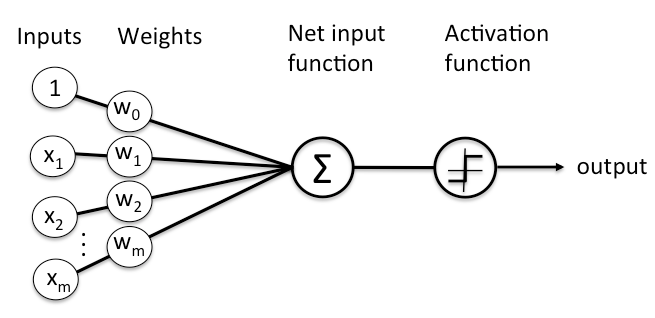
\includegraphics[width=120 mm]{images/perceptron-node.png}
	\caption{Minh họa cách hoạt động của một nơ-ron. (Nguồn: \url{https://wiki.pathmind.com/neural-network})}
	\label{fig:perceptron-node}
\end{figure}

Một hàm số phức tạp, hàm số phụ thuộc vào nhiều tham số, sẽ cần số lượng đơn vị tính toán lớn để có thể biểu diễn được tập hàm của hàm số đó. Để thoả mãn số lượng đơn vị tính toán cần thiết, các mạng nơ-ron nông thực hiện mở rộng mô hình theo chiều ngang, hay tăng số lượng nơ-ron trong tầng ẩn. Với các hàm số phức tạp, các mạng nơ-ron nông cần số lượng nơ-ron trong tầng ẩn lớn. Tuy nhiên, cách làm này dù tăng khả năng ``ghi nhớ'' nhưng lại giảm khả năng tổng quát hoá của mô hình. Điều đó có nghĩa là nếu dữ liệu huấn luyện bao gồm tất cả trường hợp có thể có của bài toán thì mạng nơ-ron nông có thể ``học thuộc lòng'' kết quả tương ứng với từng trường hợp. Chính nhược điểm đó làm giảm tính ứng dụng thực tế của mạng nơ-ron nông. Thứ nhất, ta không thể liệt kê tất cả trường hợp có thể có của một bài toán thực tế như xử lý ảnh hay xử lý ngôn ngữ tự nhiên. Thứ hai, nếu tồn tại tập dữ liệu chứa tất cả trường hợp của một bài toán thì kích thước tập dữ liệu đó là rất lớn. Thứ ba, chúng ta sẽ cần rất nhiêu nhân lực và thời gian để xây dựng nên một bộ dữ liệu như vậy.  Mạng nơ-ron nhiều tầng ẩn giải quyết vấn đề này bằng cách mở rộng mô hình theo chiều sâu, tăng số lượng tầng ẩn trung gian thay vì tăng số lượng nơ-ron cho một tầng duy nhất. Việc có nhiều tầng ẩn giúp mạng biểu diễn được các hàm phức tạp mà các mô hình học máy truyền thống không biểu diễn được. Ngoài ra, mạng nơ-ron sâu còn có thể biểu diễn được cùng một tập hàm nhưng với số lượng trọng số ít hơn mạng nơ-ron nông \cite{bengio2009learning}. Hình \ref{fig:dnn} mô tả một mạng nơ-ron nhiều tầng ẩn đơn giản với một tầng nhập, hai tầng ẩn và một tầng xuất.

\begin{figure}[H]
	\centering
	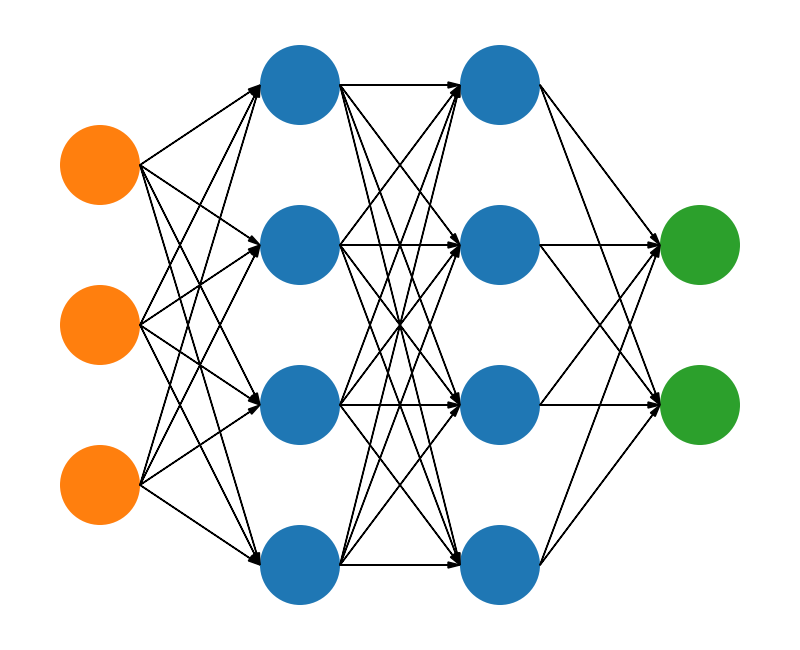
\includegraphics[width=80 mm]{images/dnn.png}
	\caption{Mô hình mạng nơ-ron nhiều tầng ẩn với tầng nhập (màu cam), các tầng ẩn (màu xanh dương) và tầng xuất (màu xanh lá)}
	\label{fig:dnn}
\end{figure}

Mô hình nhận tín hiệu đầu vào từ tầng nhập. Các tín hiệu này sẽ được truyền thẳng qua các nơ-ron ở tầng tiếp theo và tiếp tục lặp lại cho đến khi có được tín hiệu đầu ra ở tầng xuất. Quá trình này được gọi là quá trình truyền thẳng. Quá trình truyền thẳng dữ liệu qua mạng no-ron nhiều tầng ẩn cũng có thể được biểu diễn dưới dạng các hàm số được xâu chuỗi với nhau. Xét mạng nơ-ron có 2 tầng ẩn ở hình \ref{fig:dnn}, chúng ta có thể biểu diễn mô hình đó bằng công thức $\hat{y}=f^{(2)}(f^{(1)}(x))$ với $f^{(1)}$ là tầng ẩn thứ nhất và $f^{(2)}$ là tầng ẩn thứ 2, và $\hat{y}$ sẽ là giá trị cuối cùng mà mô hình dự đoán được từ dữ liệu đầu vào $x$. Qua mỗi hàm $f^{(i)}$ trung gian, dữ liệu của tầng trước sẽ bị biến đổi phi tuyến, hay ánh xạ dữ liệu sang chiều không gian khác, và truyền đến tầng tiếp theo.

\begin{figure}[H]
	\centering
	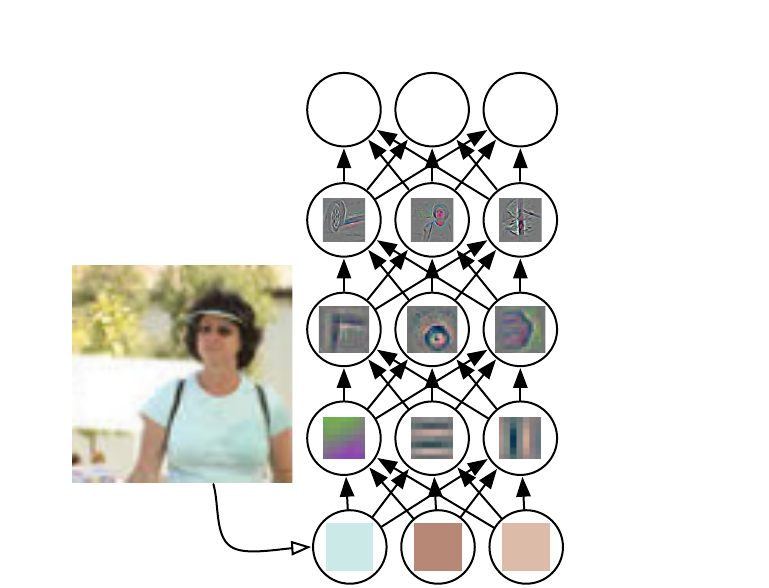
\includegraphics[width=160 mm]{images/dnn-features.png}
	\caption{Quá trình mạng nơ-ron trích xuất các đặc trưng của dữ liệu \cite{goodfellow2016deeplearning}.}
	\label{fig:dnn-features}
\end{figure}

Ngoài trích xuất được thêm thông tin, các tầng ẩn còn có khả năng rút trích các đặc trưng trung gian và kết hợp các đặc trưng đơn giản ở tầng trước đó thành các đặc trưng cấp cao hơn. Nơ-ron giữa các tầng truyền tín hiệu thông qua liên kết có trọng số. Từ đó, nơ-ron ở tầng càng sâu sẽ bị ảnh hưởng bởi các nơ-ron ở các tầng trước đó. Chính sự ảnh hưởng này giúp mạng nơ-ron nhiều tầng ẩn có thể rút trích các đặc trưng trừu tượng mà các mạng học nông khó có thể ``học'' được. Hình \ref{fig:dnn-features} cho thấy ở tầng ẩn đầu tiên, mô hình kết hợp các giá trị điểm ảnh thành các đường nét đơn giản. Sau đó ở tầng tiếp theo, các đường nét được kết hợp thành các hình khối. Từ các hình khối, mạng nơ-ron hình thành những vật thể hoàn chỉnh hơn để làm cơ sở đưa ra dự đoán. Vì vậy mà các mạng nơ-ron sâu có khả năng tổng quát hoá cao hơn các mạng nơ-ron nông có cùng số lượng nơ-ron. Như vậy, chúng ta có thể thấy được rằng, với càng nhiều tầng ẩn, mô hình mạng nơ-ron sẽ càng rút trích thông tin tốt hơn, từ đó tăng cường khả năng xử lý các bài toán phức tạp.

\section{Bài toán tối ưu hóa cần giải quyết khi huấn huyện mạng nơ-ron nhiều tầng ẩn}

Xét một bài toán học có giám sát (supervised learning), chúng ta có tập dữ liệu huấn luyện $X$ và tập giá trị đúng (ground truth) $Y$. Mô hình mạng nơ-ron là một hàm $\mathcal{F}: (\theta, x) \rightarrow \hat{y}$ với $x$ là một điểm dữ liệu và $\hat{y}$ là giá trị mà mạng nơ-ron dự đoán ra dựa theo bộ trọng số $\theta$. Như vậy, với tập dữ liệu huấn luyện $X$ và tập giá trị đúng $Y$, chúng ta sẽ tính được độ lỗi của mô hình trên toàn tập dữ liệu huấn luyện với một hàm chi phí $\mathcal{L}(\theta)$ với $\theta$ là bộ trọng số của mô hình mạng nơ-ron:

\begin{equation}
	\label{eqn:E-y}
	\mathbf{\it{E}(\theta)} = \frac{1}{N}\cdot \sum_{i=1}^{N}\mathcal{L}(\hat{y_i}, y_i)
\end{equation}
\begin{equation}
	\label{eqn:E-Fx}
	\Rightarrow \mathbf{\it{E}(\theta)} = \frac{1}{N}\cdot \sum_{i=1}^{N}\mathcal{L}(\mathcal{F}_\theta( x_i), y_i)
\end{equation}

Trong đó, $\theta$ là bộ trọng số của mô hình, $x_i = \{x_1, x_2,...x_N\}$ là tập các tín hiệu đầu vào và $N$ là kích thước tập dữ liệu huấn luyện, hàm $\mathcal{L}(\mathcal{F}_\theta( x_i), y_i)$ là hàm đánh giá độ lỗi của mạng nơ-ron với bộ trọng số $\theta$ và điểm dữ liệu $x_i$. Trung bình của các độ lỗi này là hàm chi phí $E(\theta)$ mà ta cần tối ưu. Với hàm chi phí $E(\theta)$ và không gian cao chiều được tạo bởi bộ trọng số, ta được một bề mặt phẳng lỗi $M$ chiều với $M$ là số trọng số của mạng nơ-ron.

Vì vậy, ta có thể đưa quá trình huấn luyện mạng nơ-ron thành quá trình đi tìm vị trí trong bề mặt lỗi mà tại đó hàm chi phí $E(\theta)$ đạt giá trị cực tiểu. Giá trị này có độ lỗi rất nhỏ trên tập huấn luyện, đồng thời có độ lỗi đủ nhỏ trên dữ liệu ngoài tập huấn luyện để đảm bảo tính tổng quát hóa của mô hình. Tuy nhiên, việc đi tìm giá trị cực tiểu này gặp nhiều khó khăn do bề mặt hàm lỗi xác định bởi bộ trọng số của mô hình mạng nơ-ron nhiều tầng ẩn có số chiều rất lớn. Vì vậy, cách giải phương trình thông thường không thể áp dụng trong trường hợp này. Hơn nữa, mỗi tín hiệu đầu vào có mức độ ảnh hưởng, được đặc trưng bởi giá trị trọng số, khác nhau lên độ lỗi làm xuất hiện các ``critical point'' (như điểm cực tiểu địa phương và điểm yên ngựa), các vùng bằng phẳng và vùng rãnh hẹp. Các đặc điểm này của bề mặt lỗi làm phức tạp hoá quá trình huấn luyện mạng nơ-ron nhiều tầng ẩn.

``Critical point'' (điểm tới hạn) là điểm mà tại đó hàm số không khả vi hoặc có đạo hàm bằng 0. Theo đó, cực tiểu địa phương của một hàm $f(x)$ là một điểm cực trị a trong một khoảng xác định có giá trị f(a) không lớn hơn bất kỳ giá trị $f(x)$ với mọi $x$ trong khoảng đó (hình \ref{fig:minimas}a). Công trình của D. Erhan và cộng sự \cite{erhan2009thedifficulty} đã chứng minh rằng mạng nơ-ron nhiều tầng ẩn rất dễ hội tụ tại các điểm cực tiểu có độ lỗi khá cao nếu khởi tạo ngẫu nhiên. Do đó, các điểm này từng được coi là nguyên nhân chính dẫn đến độ chính xác của mô hình bị hạn chế \cite{bengio2007scaling} và gây trở ngại trong việc ứng dụng các mô hình mạng nơ-ron nhiều tầng ẩn vào thực tế. Tuy nhiên, một số nghiên cứu gần đây cho rằng điểm cực tiểu địa phương không phải là khó khăn chính cản trở quá trình huấn luyện của mạng nơ-ron nhiều tầng ẩn mà chính các điểm yên ngựa mới là trở ngại cho các thuật toán tối ưu~\cite{dauphin2014identifying}.

\begin{figure}[htp]
	\centering
	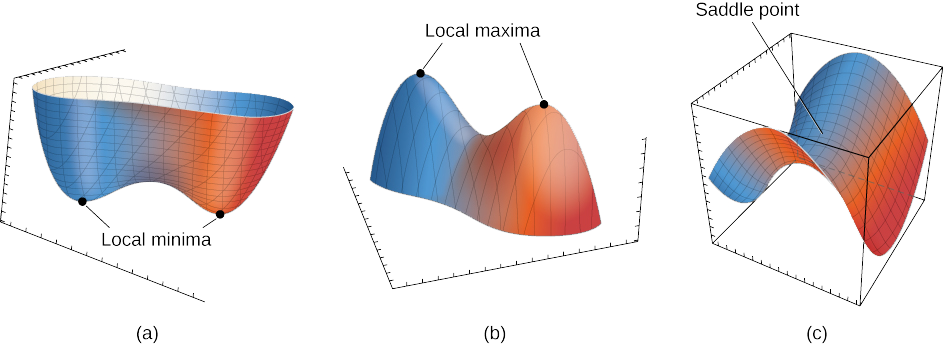
\includegraphics[width=140 mm]{images/minimas.png}
	\caption{Minh hoạ điểm cực tiểu (a), cực đại (b) và điểm yên ngựa (c) trong không gian ba chiều.}
	\label{fig:minimas}
\end{figure}

Một hàm số $f(x,y)$ có điểm dừng tại $(a,b)$ nhưng tại đó hàm số $f(x,y)$ không có cực trị, ta gọi điểm $(a,b)$ là điểm yên ngựa. Hình \ref{fig:minimas}c mô tả một điểm yên ngựa trong không gian hai chiều, cho thấy điểm yên ngựa là điểm có giá trị cực tiểu tại một chiều nhưng lại là cực đại tại một chiều khác. Trong các mạng nơ-ron nông, điểm yên ngựa chiếm tỉ lệ rất ít, đa số các critical point được tìm thấy là các cực tiểu địa phương. Tuy nhiên, Yann N. Dauphin đã chỉ ra rằng khi số lượng tầng ẩn trong mạng càng tăng thì tỉ lệ xuất hiện của các điểm yên ngựa là càng cao và gần như tất cả các critical point được tìm thấy là điểm yên ngựa có độ lỗi cao hơn rất nhiều độ lỗi của cực tiểu toàn cục \cite{dauphin2014identifying}. Đồng thời, bài báo cũng chỉ ra rằng trong không gian cao chiều, xác suất để tất cả các hướng xung quanh một critical point có đường cong lên là rất thấp, nghĩa là tần suất xuất hiện của điểm cực tiểu địa phương là rất nhỏ. Vì những lý do trên mà các điểm yên ngựa được coi là lý do lớn gây cản trở quá trình tối ưu mạng nơ-ron nhiều tầng ẩn.

Có hai khó khăn chính cần phải giải quyết khi gặp điểm yên ngựa: (1) Tìm được hướng có đường cong hướng xuống trong bề mặt lỗi để tiến tới điểm có độ lỗi nhỏ hơn, và (2) vượt qua vùng bằng phẳng, là vùng có độ dốc gần như bằng nhau theo tất cả các hướng, bao bọc xung quanh điểm yên ngựa. Trong các thuật toán tối ưu sử dụng đạo hàm bậc nhất, mặc dù tìm được hướng tới điểm có độ lỗi nhỏ hơn, nhưng các bước cập nhật diễn ra rất chậm do độ dốc của các điểm này rất nhỏ và dường như bằng nhau trong vùng lân cận. Để khắc phục được khó khăn này, một số thuật toán bậc nhất đã cố gắng xấp xỉ thông tin đạo hàm bậc hai để có thêm thông tin về độ cong của bề mặt lỗi tại điểm đang xét. Các thuật toán này đều là những cải tiến của thuật toán Gradient Descent.

\section{Thuật toán tối ưu Gradient Descent}

\begin{figure}[H]
	\centering
	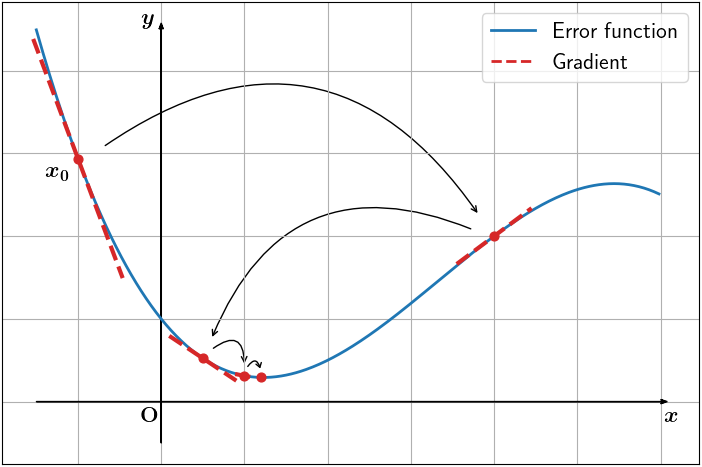
\includegraphics[width=140 mm]{images/gd.png}
	\caption{Minh họa quá trình tìm đến điểm cực tiểu của thuật toán Gradient Descent với đường màu xannh dương biểu diễn giá trị của hàm chi phí, đường đứt đoạn màu đỏ thể hiện phương và độ lớn của gradient.}
	\label{fig:gd}
\end{figure}

``Gradient Descent'' là thuật toán cho phép đi tìm cực tiểu của một hàm số mà không cần biết chính xác công thức của hàm số đó bằng cách di chuyển từng bước nhỏ cho đến khi hội tụ tại cực tiểu (hình \ref{fig:gd}). Bằng cách sử dụng khai triển Taylor, ta có thể xấp xỉ đạo hàm bậc k của bất kỳ hàm số nào, cho phép Gradient Descent giải quyết được hầu hết các hàm số được dùng trong huấn luyện mạng nơ-ron nhiều tầng ẩn.

\begin{itemize}
	\item Khai triển Taylor: Công thức \ref{eqn:taylor-f} cho xấp xỉ đạo hàm bậc $k$ của một hàm số $f(x)$ quanh một điểm $x$ với $\Delta x$ đủ nhỏ.
	\begin{equation} \label{eqn:taylor-f}
		f(x + \Delta x) \approx f(x) + f'(x)\Delta x + \frac{1}{2!}f''(x)(\Delta x)^2 +...+ \frac{1}{k!}f^{(k)} (\Delta x)^{(k)}
	\end{equation}
	Từ đó, để có thể cực tiểu hóa hàm chi phí $\mathcal{L}$, Gradient Descent sẽ di chuyển theo hướng $\Delta x$ sao cho $\mathcal{L}(x + \Delta x) < \mathcal{L}(x)$ và bằng:
	\begin{equation} \label{eqn:Lx-delta1}
		\mathcal{L}(x + \Delta x) \approx \mathcal{L}(x) + \Delta x\nabla_x \mathcal{L}
	\end{equation}
	với $\nabla_x\mathcal{L}$ là gradient của hàm chi phí $\mathcal{L}$ tại $x$.

	\item Gradient là véc-tơ có hướng là hướng có mức độ tăng lớn nhất và độ lớn là mức độ thay đổi lớn nhất tại một điểm trong không gian. Giả sử một không gian $\mathbb{R}^n$ được định nghĩa bởi một hàm $f(x_1,x_2,x_3,...,x_n)$ thì véc-tơ gradient tại một điểm trong không gian $\mathbb{R}^n$ sẽ là một véc-tơ cột mà thành phần của nó là đạo hàm theo từng biến của hàm $f(x_1,x_2,x_3,...,x_n)$, cụ thể là:
	\begin{equation} \label{eqn:gradf}
		\nabla f = (\frac{\delta f}{\delta x_1}, \frac{\delta f}{\delta x_2}, \frac{\delta f}{\delta x_3},...,\frac{\delta f}{x_n})
	\end{equation}
\end{itemize}

Vì gradient chỉ hướng có mức độ tăng lớn nhất nên hướng $\Delta x$ cho giá trị của $\mathcal{L} (x + \Delta x)$ giảm nhiều nhất theo hướng $-\nabla_x\mathcal{L}$. Tuy nhiên, $\Delta x$ phải có giá trị đủ nhỏ để xấp xỉ Taylor vẫn đảm bảo rằng hướng $\Delta x$ sẽ cho giá trị $\mathcal{L}(x + \Delta x) < \mathcal{L}(x)$. Từ đó, ta áp dụng một hằng số dương $\eta$ đảm bảo độ dài của một bước đi $\Delta x$ đủ nhỏ, được gọi là tỷ lệ học (learning rate). Vậy ta có thể viết được công thức cập nhật của Gradient Descent tại mỗi bước nhảy $x_t$ như sau:

\begin{equation}
	\label{eqn:Lx-delta2}
	\mathcal{L}(x_t + \Delta x) \approx \mathcal{L}(x_t) - \eta{(\nabla_{x_t} \mathcal{L})^T\nabla _{x_t}\mathcal{L}}
\end{equation}
Lại có: $(\nabla _{x_t}\mathcal{L})^T\nabla _{x_t} \mathcal{L} > 0 \Rightarrow \mathcal{L}(x_t + \Delta x) < \mathcal{L}(x_t)$.

Với hằng số $\eta$ cố định công thức \ref{eqn:Lx-delta1} sẽ luôn ftiến hành cập nhật một lượng $\Delta x = \eta (\nabla _{x_t}\mathcal{L})^T\nabla _{x_t}\mathcal{L} = \eta ||\nabla _{x_t}\mathcal{L}||_2$ thay đổi tương ứng tỷ lệ với $||\nabla _{x_t} \mathcal{L}||_2$. Nếu $||\nabla _{x_t} \mathcal{L}||_2$ lớn, có nghĩa là độ dốc lớn, ta có thể bước một bước dài để tiến nhanh tới giá trị cực tiểu. Ngược lại, nếu $||\nabla_{x_t} \mathcal{L}||_2$ nhỏ, độ dốc nhỏ, ta phải bước những bước nhỏ để tránh bị vượt qua khỏi vùng cực tiểu.

Bên cạnh đó, nếu tỷ lệ học quá nhỏ, ta luôn bước những bước rất nhỏ hướng về phía cực tiểu nên sẽ mất rất nhiều thời gian để thuật toán có thể hội tụ. Tuy nhiên, nếu chọn một tỷ lệ học quá lớn thì xấp xỉ Taylor không đảm bảo được rằng giá trị $\mathcal{L}(x + \Delta x)$ sẽ giảm và thuật toán có khả năng không thể hội tụ. Đó là lý do tại sao lựa chọn một tỷ lệ học phù hợp là cần thiết.

Từ công thức \ref{eqn:E-Fx} và \ref{eqn:Lx-delta2}, ta có thể viết được công thức cập nhật của $\theta$ tại mỗi bước:

\begin{equation}
	\label{eqn:theta-batch-update}
	\theta_{t+1} = \theta_ t - \eta \nabla_{\theta} \mathbf{\it{E}(\theta)}
\end{equation}
với $\nabla_\theta \mathbf{\it{E}(\theta)}$ là gradient của hàm chi phí được tính trên toàn tập dữ liệu.

Tổng quan thuật toán GD được trình bày trong thuật toán \ref{alg:GD}.

\begin{algorithm}
	\caption{Gradient Descent (GD)} \label{alg:GD}
	\begin{algorithmic}[1]
		\renewcommand{\algorithmicrequire}{\textbf{Đầu vào:}}
		\renewcommand{\algorithmicensure}{\textbf{Đầu ra:}}
		\algnewcommand\algorithmicoperation{\textbf{Thao tác:}}
		\algnewcommand\Operation{\item[\algorithmicoperation]}

		\Require Tập dữ liệu huấn luyện $x_i (i = 1, 2, ..., N)$, tỉ lệ học $\eta$, bộ trọng số $\theta$ của mô hình $\mathcal{F}$
		\Ensure Bộ trọng số $\theta$ của $\mathcal{F}$ với độ lỗi đạt cực tiểu

		\Operation
		\While{$\theta$ chưa hội tụ}
			\State Tính độ lỗi trung bình: $\mathbf{\it{E}(\theta)} = \frac{1}{N}\cdot \displaystyle\sum_{i=1}^{N}\mathcal{L}(\hat{y_i}, y_i)$
			\State Thực hiện cập nhật trọng số: $\theta = \theta - \eta \nabla_{\theta} \mathbf{\it{E}(\theta)}$
		\EndWhile
		\State return $\theta$
	\end{algorithmic}
\end{algorithm}

\section{Thuật toán tối ưu Stochastic Gradient Descent}

Một trong những trở ngại của GD khi ứng dụng vào việc huấn luyện mạng nơ-ron nhiều tầng ẩn là tốc độ huấn luyện. Việc huấn luyện một mạng nơ-ron nhiều tầng ẩn thường đòi hỏi một tập dữ liệu rất lớn để mô hình có thể học đủ thông tin về các đặc trưng của dữ liệu. Trong mỗi bước, GD cần duyệt qua từng điểm dữ liệu trong tập dữ liệu huấn luyện, tính độ lỗi và véc-tơ đạo hàm riêng của độ lỗi theo từng trọng số, cuối cùng là tính trung bình của các véc-tơ đạo hàm để có được véc-tơ gradient $\nabla_{\theta}\mathbf{\it{E}}(\theta)$, và chúng ta chỉ dùng một phần nhỏ của độ dài gradient đó để cập nhật.

Có thể thấy GD mất rất nhiều thời gian để duyệt qua hết toàn bộ tập dữ liệu, nhưng chỉ cải thiện được một lượng rất nhỏ. Để khắc phục nhược điểm này, Stochastic Gradient Descent (SGD) chỉ thực hiện tính gradient của hàm chi phí trên một tập con của tập dữ liệu (thường gọi là một ``minibatch'') để thực hiện một bước cập nhật.

Từ công thức \ref{eqn:Lx-delta2} và \ref{eqn:theta-batch-update} của GD, chúng ta sẽ có công thức tính độ lỗi của SGD với một tập con:

\begin{equation}
	\label{eqn:E-minibatch}
	\mathbf{\it{E}(\theta)} = \frac{1}{k}\cdot \sum_{i=1}^{k}\mathcal{L}(\mathcal{F}_\theta( x_i), y_i)
\end{equation}
với $k$ là kích thước của một tập con ($k<<N$). Từ độ lỗi tính được, việc cập nhật trọng số cho mạng nơ-ron nhiều tầng ẩn được thực hiện tương tự như GD bằng công thức \ref{eqn:theta-batch-update}.

Như vậy, có thể thấy được rằng một bước cập nhật với SGD sẽ nhanh hơn rất nhiều so với GD do việc tính toán chỉ thực hiện trên $k$ điểm dữ liệu và cập nhật theo gradient của tập con đó. Ngoài ra, trong mỗi lần duyệt qua toàn bộ tập dữ liệu (gọi là một ``epoch''), SGD thực hiện được $N/k$ lần cập nhật trọng số cho mô hình, thay vì chỉ một lân như GD. Điều đó cũng đồng nghĩa rằng với cùng một số lượng epoch huấn luyện, SGD sẽ đi được rất nhiều bước so với GD.

\begin{figure}[H]
	\centering
	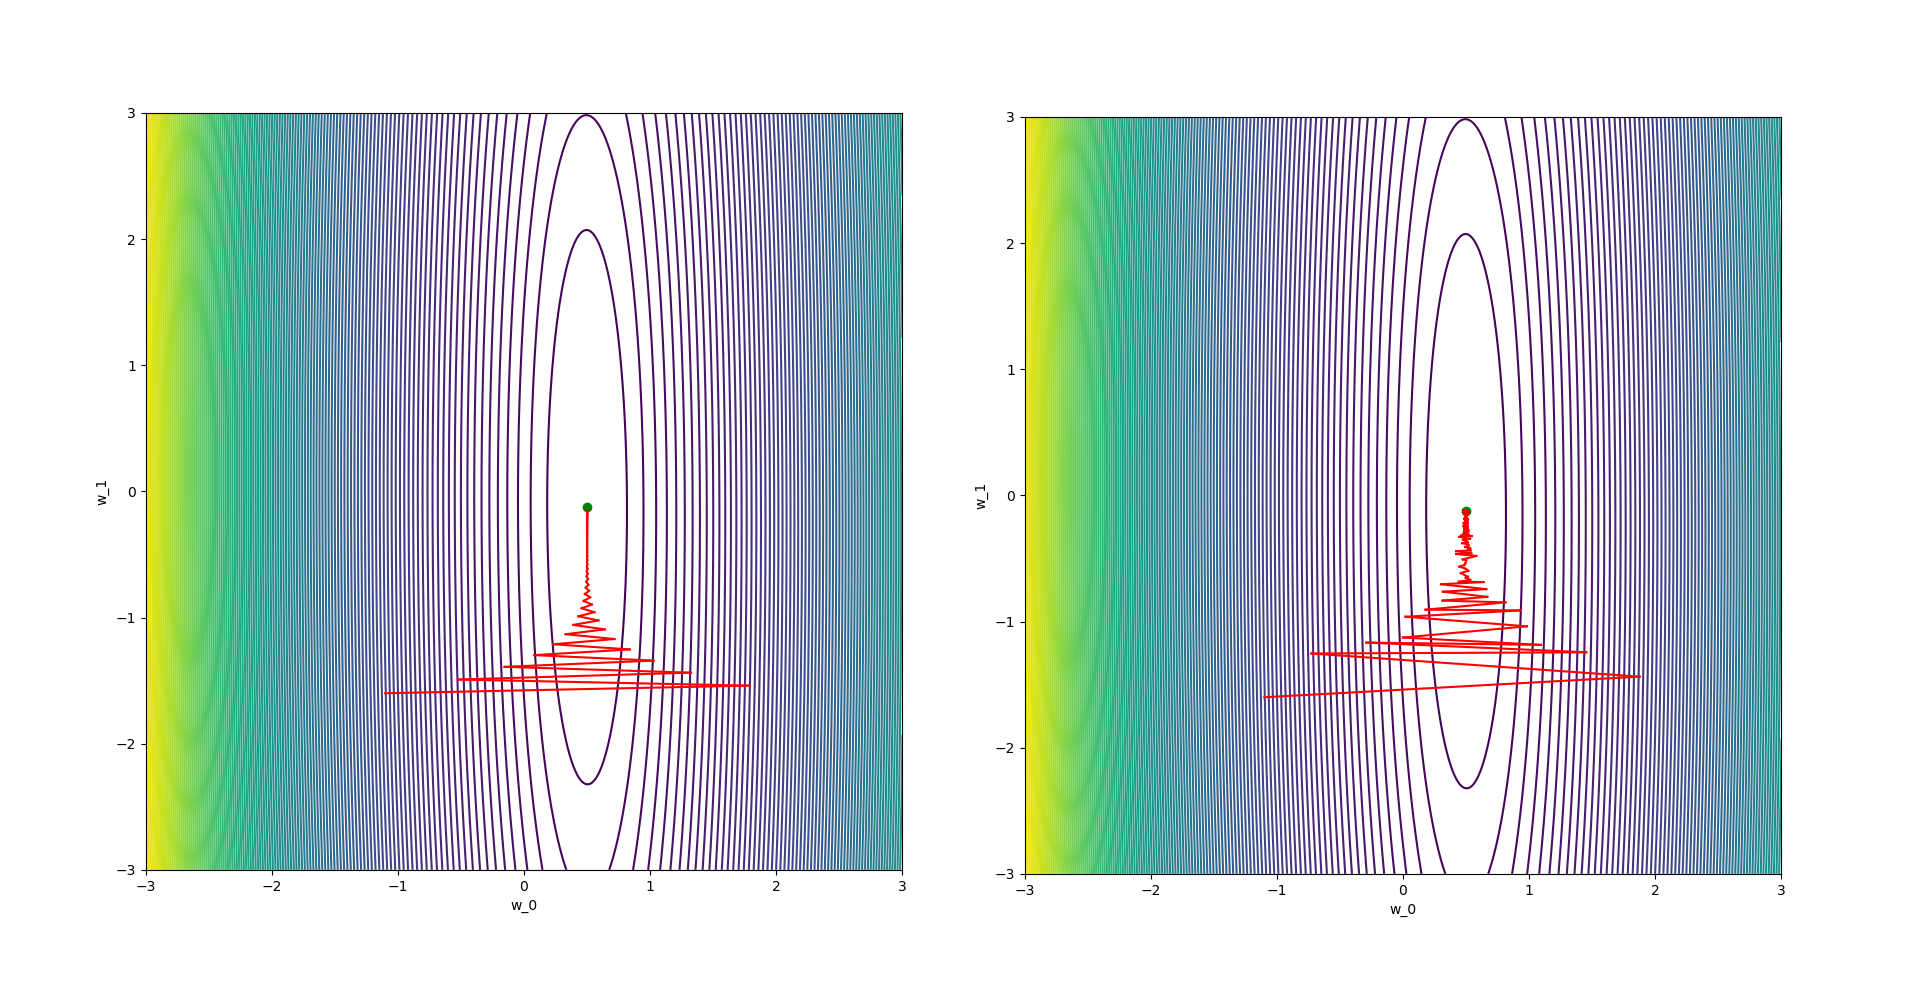
\includegraphics[width=140 mm]{images/gd-sgd.png}
	\caption{So sánh đường đi của Gradient Descent (trái) và Stochastic Gradient Descent (phải).}
	\label{fig:gd-sgd}
\end{figure}

Việc chỉ sử dụng một tập con của dữ liệu huấn luyện để tính gradient cũng đồng nghĩa với việc hướng của gradient này sẽ chỉ xấp xỉ gradient tính được trên cả tập dữ liệu (có thể gọi là ``true gradient''), và sẽ có những sự dao động. Tuy nhiên, nhiều nghiên cứu đã chỉ ra rằng các véc-tơ gradient của các tập con sẽ dao động xung quanh hướng của véc-tơ gradient tính được theo GD với độ chênh lệch không quá lớn (hình \ref{fig:gd-sgd}) \cite{bottou2010large}\cite{bottou2018optimization}. Việc lựa chọn kích thước tập con $k$ là sự đánh đổi giữa mức độ dao động với tốc độ tính toán cũng như số bước cập hật được thực hiện trong mỗi epoch. Khi $k$ tiến tới gần $N$, hướng gradient của tập con sẽ xấp xỉ hướng của true gradient tốt hơn, nhưng lại mất nhiều thời gian tính toán hơn. Ngược lại, khi $k$ tiến gần về 1, tuy thời gian tính toán được rút ngắn nhưng hướng gradient của tập con càng chênh lệch nhiều so với hướng của true gradient, gây ra sự nhiễu loạn.

Tổng quan thuật toán SGD được trình bày trong thuật toán \ref{alg:SGD}.

\begin{algorithm}
	\caption{Stochastic Gradient Descent (SGD)} \label{alg:SGD}
	\begin{algorithmic}[1]
		\renewcommand{\algorithmicrequire}{\textbf{Đầu vào:}}
		\renewcommand{\algorithmicensure}{\textbf{Đầu ra:}}
		\algnewcommand\algorithmicoperation{\textbf{Thao tác:}}
		\algnewcommand\Operation{\item[\algorithmicoperation]}

		\Require Tập dữ liệu huấn luyện $x_i (i = 1, 2, ..., N)$, kích thước tập con $k$, tỉ lệ học $\eta$, bộ trọng số $\theta$ của mô hình $\mathcal{F}$
		\Ensure Bộ trọng số $\theta$ của $\mathcal{F}$ với độ lỗi đạt cực tiểu

		\Operation
		\While{$\theta$ chưa hội tụ}
			\State Xáo trộn tập dữ liệu.
			\For{mỗi tập con kích thước $k$}
				\State Tính độ lỗi trung bình: $\mathbf{\it{E}(\theta)} = \frac{1}{k}\cdot \displaystyle\sum_{i=1}^{k}\mathcal{L}(\hat{y_i}, y_i)$
				\State Thực hiện cập nhật trọng số: $\theta$ = $\theta - \eta \nabla_{\theta} \mathbf{\it{E}(\theta)}$
			\EndFor
		\EndWhile
		\State return $\theta$
	\end{algorithmic}
\end{algorithm}

\section{``Lan truyền ngược'' (Backpropagation)}

Quá trình huấn luyện mạng nơ-ron cần tìm một bộ trọng số cho độ lỗi là nhỏ nhất và việc tìm kiếm này có thể được hoàn thành bằng các thuật toán tối ưu đã trình bày ở trên. Tuy nhiên các thuật toán tối ưu này cần véc-tơ đạo hàm riêng của hàm chi phí tại từng trọng số, có nghĩa là ta muốn tìm sự phụ thuộc của độ lỗi và các giá trị trọng số trong mạng. Thuật toán lan truyền ngược có thể giải quyết được vấn đề này bằng cách ``lan truyền'' độ lỗi trở lại trong mạng, từ đó có thể thay đổi giá trị của các trọng số tương ứng với mức độ ảnh hưởng lên độ lỗi. Ý tưởng cho thuật toán được giới thiệu trong bài báo của nhóm tác giả David Rumelhart, Geoffrey Hinton và Ronald Williams dưới cái tên Generalized Delta Rule \cite{rumelhart1986learning}. Thuật toán ra đời đã đánh dấu một sự phát triển vượt bậc trong việc huấn luyện mạng nơ-ron nhiều tầng ẩn và nhận được sự quan tâm rất lớn trong cộng đồng nghiên cứu.

Thuật toán lan truyền ngược là một phép vi phân ngược (reverse-mode differentiation) sử dụng quy tắc mắt xích (chain rule) để tính toán mức độ ảnh hưởng của một trọng số lên giá trị độ lỗi của mạng nơ-ron nhiều tầng ẩn và được thể hiện qua giá trị độ lớn của các phần tử trong véc-tơ $\nabla_\theta \mathbf{\it{E}(\theta)}$ tương ứng cho từng trọng số. Nếu một phần tử trong véc-tơ $\nabla_\theta \mathbf{\it{E}(\theta)}$ có giá trị lớn, nghĩa là khi thay đổi trọng số tương ứng một lượng nhỏ thì độ lỗi sẽ thay đổi một lượng lớn, và ngược lại, nếu một phần tử trong $\nabla_\theta \mathbf{\it{E}(\theta)}$ có giá trị nhỏ bị thay đổi thì độ lỗi sẽ chỉ biên thiên một lượng nhỏ. Vì tính chất đó mà ta gọi giá trị này là ``độ nhạy cảm'' của trọng số.

``Độ nhạy cảm'' của một trọng số $w_i \in \theta$ được tính bằng tỉ lệ giữa độ biến thiên của trọng số đó và độ biến thiên của hàm chi phí $\mathbf{\it{E}(\theta)}$ và bằng đạo hàm riêng của hàm $\mathbf{\it{E}(\theta)}$ tại từng trọng số: $\frac{\delta E}{\delta w_1}; \frac{\delta E}{\delta w_2};...;\frac{\delta E}{\delta w_n}$. Tổng hợp của các giá trị này cho ta véc-tơ $\nabla_\theta \mathbf{\it{E}(\theta)}$. Để dễ dàng trong việc giải thích cách thuật toán thực thi, ta sử dụng một mạng nơ-ron nhiều tầng ẩn đơn giản, được mô tả như hình \ref{fig:wandb} với 1 tầng nhập, 2 tầng ẩn và 1 tầng xuất, mỗi tầng chỉ có một nơ-ron.

\begin{figure}[htp]
	\centering
	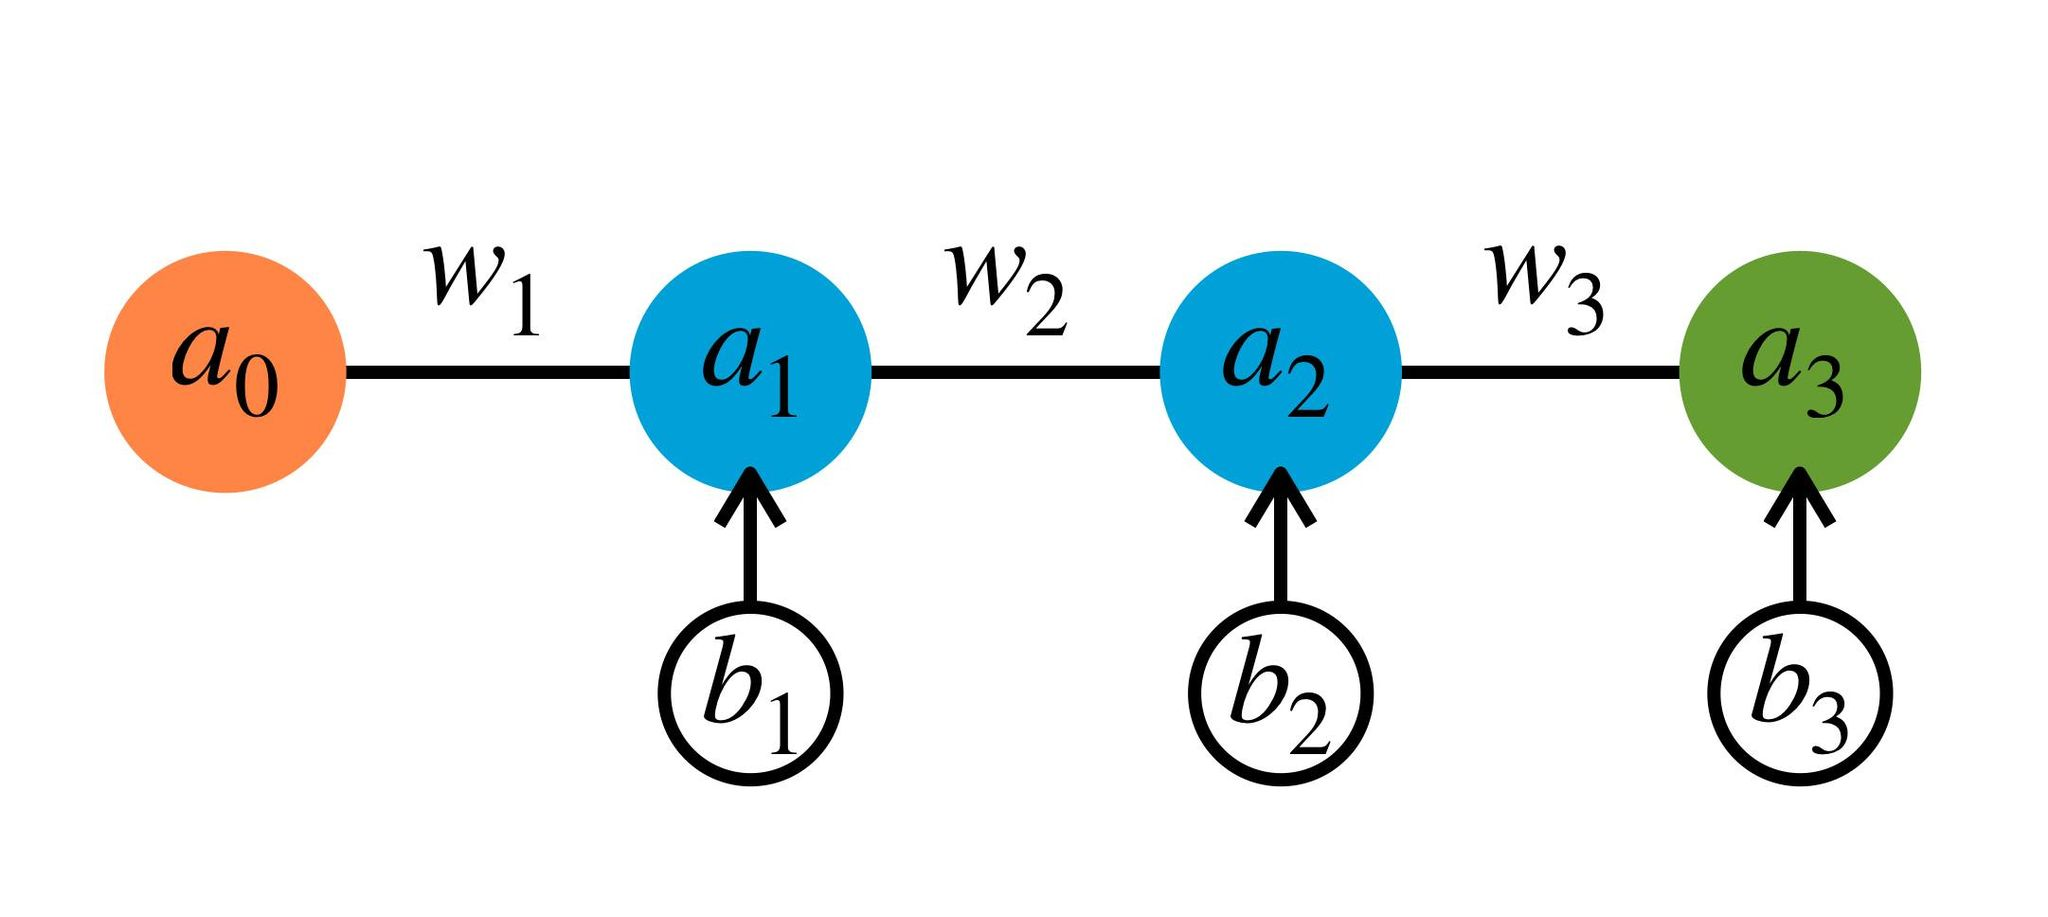
\includegraphics[width=140 mm]{images/wandb.jpg}
	\caption{Minh họa mô hình mạng nơ-ron đơn giản gồm ba tầng: 1 tầng nhập (màu cam), 2 tầng ẩn (màu lam) và 1 tầng xuất (màu lục). Trong đó, $w_i$ là các trọng số liên kết, $b_i$ là hệ số bias tương ứng của từng nơ-ron và $a_i$ là giá trị kích hoạt của nơ-ron.}
	\label{fig:wandb}
\end{figure}

Khi ta truyền tín hiệu đầu vào $a_0$ vào mô hình, sau khi rút trích đặc trưng qua 2 tầng ẩn, ta được kết quả dự đoán ở $a_3$. Đem so sánh kết quả tại $a_3$ với giá trị nhãn đúng $y$ ta được độ lỗi $E(\theta)$ được tính bằng công thức sau:

\begin{equation}
	\begin{cases}
		E(\theta) = (a_3 - y)^2 \\
		a_3 = \sigma(w_3\cdot a_2 + b_3)
	\end{cases} \\
	\rightarrow E(\theta) = (\sigma(w_3\cdot a_2 + b_3) - y)^2
\end{equation}

Từ độ lỗi này, ta cần tìm đạo hàm riêng của $E(\theta)$ theo từng trọng số. Theo quy tắc mắt xích, ta có:

\begin{equation}
	\label{eqn:chain1}
	\begin{split}
		\frac{\delta E}{\delta w_3} &= \frac{\delta E}{\delta \sigma}\cdot\frac{\delta \sigma}{\delta (w_3a_2 + b_3)}\cdot \frac{\delta(w_3a_2 + b_3)}{\delta w_3} \\ &= 2(\sigma(w_3a_2+b_3)-y). \sigma(w_3a_2 + b_3)'\cdot a_2
	\end{split}
\end{equation}
với $\sigma(x)$ là một hàm kích hoạt bất kỳ. Đặt $z_3 = \theta_3a_2 + b_3$, ta viết lại công thức \ref{eqn:chain1}:

\begin{equation}
	\label{eqn:chain2}
	\frac{\delta E}{\delta w_3} = 2(\sigma(z_3)-y)\cdot \sigma(z_3)\cdot a_2
\end{equation}

Tương tự như vậy, ta có đạo hàm riêng của $E(\theta)$ tại $w_1$ và $w_2$:

\begin{equation}
	\label{eqn:chain3}
	\begin{split}
		\frac{\delta E}{\delta w_2} &= \frac{\delta E}{\delta \sigma(z_2)}\cdot\frac{\delta \sigma(z_2)}{\delta z_2}\cdot\frac{\delta z_2}{\delta w_2} \\
		&= 2(\sigma(z_3)-y)\cdot \sigma(z_3)'.w_3\cdot\sigma(z_2)'\cdot a_1
	\end{split}
\end{equation}
\begin{equation}
	\label{eqn:chain4}
	\begin{split}
		\frac{\delta E}{\delta w_1} &= \frac{\delta E}{\delta \sigma(z_1)}\cdot\frac{\delta \sigma(z_1)}{\delta z_1}\cdot\frac{\delta z_1}{\delta w_1} \\
		&= 2(\sigma(z_3)-y)\cdot \sigma(z_3)'\cdot w_3\cdot\sigma(z_2)'.w_2\cdot\sigma(z_1)'\cdot a_0
	\end{split}
\end{equation}

Các công thức \ref{eqn:chain2}, \ref{eqn:chain3} và \ref{eqn:chain3} được truyền qua tập dữ liệu và lấy giá trị trung bình. Tổng hợp các giá trị này ta được véc-tơ đạo hàm riêng $\nabla_\theta \mathbf{\it{E}(\theta)}$ được dùng trong các thuật toán tối ưu khác. Tổng quát hoá cho một mô hình có $L$ tầng và số lượng nơ-ron ở mỗi tầng là $n^{(l)}$ thì độ phụ thuộc của giá trị độ lỗi vào trọng số liên kết giữa nơ-ron thứ $k$ của tầng thứ $l-1$ và nơ-ron thứ $j$ của tầng thứ $l$ là $w_{jk}$, với $z_j = ...+w_{jk}a^{l-1}_k+... + b_j$, ta có:

\begin{equation}
	\label{eqn:chain5}
	\frac{\delta E}{\delta w_{jk}} = \frac{\delta E}{\delta \sigma(z_j)} \cdot\frac{\delta \sigma(z_j)}{\delta z_j}\cdot\frac{\delta z_j}{\delta w_{jk}}
\end{equation}
và đạo hàm riêng của độ lỗi tại nơ-ron thứ $k$ của tầng thứ $l - 1$ là giá trị tổng hợp của các hàm kích hoạt của tầng thứ $l$.

\begin{equation}
	\label{eqn:chain6}
	\frac{\delta E}{\delta a_k^{l-1}} = \sum_{j=0}^{n^{l}-1}\frac{\delta E}{\delta \sigma(z_j)}\cdot\frac{\delta \sigma(z_j)}{\delta z_j}\cdot\frac{\delta z_j}{\delta a_k^{l-1}}
\end{equation}

Từ các công thức ta có thể nhận thấy rằng đây là quá trình cho một độ lỗi nhất định, không có công thức chung cho tất cả giá trị độ lỗi và toàn bộ quá trình sẽ phải được lặp lại khi có một độ lỗi mới. Đây là một điểm yếu của phương pháp vi phân ngược nhưng lại rất thích hợp trong huấn luyện mạng nơ-ron nhiều tầng ẩn.

\chapter{Huấn luyện mạng nơ-ron nhiều tầng ẩn bằng thuật toán Adam}
\label{Chapter3}

\textit{Chương này trình bày về thuật toán Adam được đề xuất bởi \cite{kingma2014adam} để giải quyết bài toán huấn luyện mạng nơ-ron nhiều tầng ẩn; đây là thuật toán mà khóa luận tập trung tìm hiểu. Đầu tiên, chúng tôi trình bày về các thuật toán nền tảng: (1) thuật toán Stochastic Gradient Descent với Momentum để tăng tốc và giảm dao động trong quá trình di chuyển trên bề mặt lỗi, và (2) thuật toán Stochastic Gradient Descent với tỉ lệ học thích ứng cho từng trọng số để có thể di chuyển tốt trong trường hợp bề mặt lỗi có độ cong khác nhau nhiều theo các hướng ứng với các trọng số. Sau đó, chúng tôi trình bày về thuật toán Adam - một cách kết hợp hai thuật toán đã nói lại để giúp giải quyết tốt hơn bài toán huấn luyện mạng nơ-ron nhiều tầng ẩn.}

\section{Thuật toán Gradient Descent với Momentum}

Các thuật toán sử dụng gradient như GD và SGD gặp phải hai khó khăn chính khi thiếu đi thông tin về độ cong của bề mặt lỗi. Đầu tiên, vì hướng của gradient là hướng có độ dốc lớn nhất nên không phải lúc nào cũng là hướng tốt nhất và có thể gây dao động mạnh trong khi độ lỗi giảm không nhiều. Thứ hai, ``độ nhạy cảm'' của mỗi trọng số là khác nhau trong bề mặt lỗi, vì vậy áp dụng một tỷ lệ học chung cho tất cả các trọng số sẽ khiến cho hướng cập nhật bỏ qua các trọng số có ``độ nhạy cảm'' nhỏ.

``GD/SGD với Momentum'' (hay ``Momentum'') là một phương pháp cải tiến sử dụng quán tính để điều chỉnh hướng gradient theo hướng tốt nhất về cực tiểu, từ đó tăng tốc độ di chuyển trên bề mặt lỗi. Quán tính được thêm vào công thức thông qua hệ số quán tính $\beta$. Tại mỗi bước $t$, véc-tơ quán tính $m_t$ được xác định bởi công thức \ref{eqn:mt}:

\begin{equation}
	\label{eqn:mt}
	m_t = \beta m_{t-1} + \eta\nabla_\theta E(\theta_t)
\end{equation}
với $m_{t-1}$ là véc-tơ quán tính trước đó, $\eta$ là tỉ lệ học và $\nabla_\theta E(\theta_t)$ là gradient của hàm chi phí tại $\theta_t$.

Từ công thức \ref{eqn:mt} ta có công thức cập nhật $\theta$ tại mỗi bước được cải tiến như sau:

\begin{equation}
	\label{eqn:theta-momentum}
	\theta_t = \theta_{t-1} - v_t
\end{equation}

Nhờ vào sự cải tiến đơn giản này mà thuật toán Momentum có thể giảm bớt sự di chuyển tại những hướng mà dấu của gradient không ổn định, đồng thời tăng cường sự di chuyển tại hướng mà dấu của gradient ổn định. Mức độ điều chỉnh sự di chuyển phụ thuộc vào hệ số quán tính $\beta$. Một hệ số $\beta$ quá lớn cũng như quá nhỏ đều kéo dài thời gian huấn luyện của mô hình. Nếu $\beta$ được chọn quá lớn thì mức độ thay đổi quá lớn dẫn đến thuật toán bị dao động quanh điểm cực tiểu; nếu $\beta$ chọn quá nhỏ, thuật toán Momentum sẽ suy biến về GD và khó khăn sẽ không được khắc phục.

Có thể nói hệ số quán tính cho phép thuật toán ưu tiên các giá trị quán tính gần hơn các giá trị quán tính cũ nhờ vào đường trung bình động hàm mũ (Exponential Moving Averages) hay EMA. Đường trung bình động hàm mũ cho phép ta sử dụng trung bình động để xử lý nhiễu trong dữ liệu mà ta quan sát được và xấp xỉ nó gần hơn với dữ liệu thực. Ta thực hiện lấy trung bình trên $\frac{1}{1-\beta}$ bước nhảy gần nhất và cập nhật trọng số. Ta khai triển công thức \ref{eqn:mt} như sau:

\begin{equation}
	\label{eqn:m3}
	\begin{aligned}
		m_1 &= \beta m_0 + \eta\nabla_\theta E(\theta_1) \\ m_2 &= \beta m_1 + \eta \nabla_\theta E(\theta_2) = \beta (m_0 + \eta\nabla_\theta E(\theta_1)) + \eta\nabla_\theta E(\theta_2) \\ &= \beta m_0 + \beta\eta\nabla_\theta E(\theta_1) + \eta\nabla_\theta E(\theta_2) \\ m_3 &= \beta m_2 + \eta\nabla_\theta E(\theta_3) = \beta (\beta m_0 + \beta\eta\nabla_\theta E(\theta_1) + \eta\nabla_\theta E(\theta_2)) + \eta\nabla_\theta E(\theta_3) \\ &= \beta^2 m_0 + \beta^2\eta \nabla_\theta E(\theta_1) + \beta \eta \nabla_\theta E(\theta_2) +\eta \nabla_\theta E(\theta_3)
	\end{aligned}
\end{equation}

Từ công thức \ref{eqn:m3} ta nhận thấy rằng tại bước nhảy thứ $t$, giá trị của véc-tơ quán tính phụ thuộc vào các giá trị véc-tơ quán tính trước đó từ $1..(t-1)$. Mỗi giá trị trong dãy đều được nhân với hệ số $\beta ^t$. Vì $\beta$ là hệ số quán tính nằm trong khoảng $(0,1)$ nên $\beta^t$ sẽ càng nhỏ khi $t$ càng lớn dẫn đến các giá trị càng lâu trước đó sẽ có hệ số càng nhỏ và dần không đóng góp gì nhiều trong quá trình huấn luyện. Hay nói cách khác, các giá trị này dần được quên đi và thuật toán Momentum quan tâm nhiều đến các giá trị gần với hiện tại.

Trong thực tế huấn luyện, ta thường sử dụng cách xấp xỉ true gradient bằng các gradient của tập con để tăng tốc quá trình cập nhật trọng số. Trong quá trình xấp xỉ, việc tạo minibatch bằng cách gom nhóm ngẫu nhiên các điểm dữ liệu đã thêm một lượng nhiễu vào trong quá trình tối ưu. So sánh độ lớn của nhiễu với độ lớn của véc-tơ quán tính ta có thể chia quá trình thành hai giai đoạn: giai đoạn ``transient'' và giai đoạn ``fine-tuning''. Trong giai đoạn transient, véc-tơ quán tính vẫn còn hiệu quả trong điều chỉnh hướng của gradient và giúp gradient tiến nhanh về vị trí có cực tiểu vì độ lớn của véc-tơ quán tính lớn hơn độ lớn của nhiễu. Quá trình huấn luyện càng lâu, độ lớn của véc-tơ quán tính ngày càng giảm và bị lấn át bởi độ nhiễu, khi đó ta bước qua giai đoạn fine-tuning. Trong các mạng nơ-ron nhiều tầng ẩn, giai đoạn fine-tuning chiếm một phần ít hơn và cũng ít quan trọng hơn giai đoạn transient nên việc đảm bảo giai đoạn transient được diễn ra đủ lâu là một sự cần thiết \cite{sutskever2013onti}.

Sự chuyển đổi giữa hai quá trình được kể trên được quyết định bởi hằng số quán tính $\beta$. Sử dụng một hệ số quán tính $\beta$ lớn cho phép Momentum thực hiện quá trình tối ưu tốt hơn trên các hướng có ``độ nhạy cảm'' nhỏ. Tuy nhiên, lợi thế này không được thể hiện qua rõ ràng qua độ lỗi do thuật toán không thể hội tụ tốt tại các hướng có ``độ nhạy cảm'' cao với một hệ số quán tính $\beta$ lớn. Sự đánh đổi này cho kết quả là ta có thể tiến gần đến vùng có cực tiểu hoặc là hội tụ tại cực tiểu có độ lỗi nhỏ hơn. Trong khi sử dụng một hệ số $\beta$ nhỏ sẽ cho độ lỗi cao hơn vì giai đoạn transient kết thúc quá sớm. Thiếu đi sự hỗ trợ của quán tính, các phương pháp bậc nhất không thể tận dụng tốt thông tin tại các hướng có ``độ nhạy cảm'' nhỏ và rất dễ bỏ qua các vùng chứa cực tiểu hoặc cực tiểu có độ lỗi thấp hơn dẫn đến hội tụ tại điểm có độ lỗi cao.

\begin{figure}[htp]
	\centering
	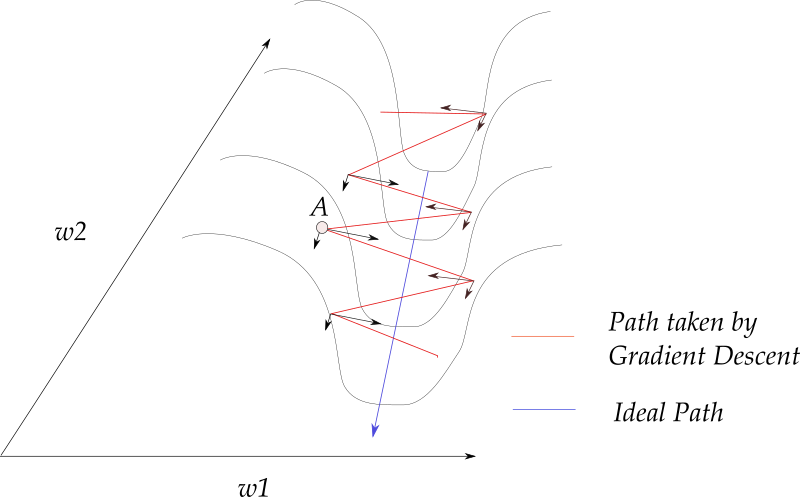
\includegraphics[width=140 mm]{images/valley-momentum.png}
	\caption{Minh họa cách Momentum triệt tiêu hướng có độ dốc lớn. (Nguồn: \url{https://blog.paperspace.com/intro-to-optimization-momentum-rmsprop-adam/})}
	\label{fig:valley-momentum}
\end{figure}

Hình \ref{fig:valley-momentum} mô tả một rãnh hẹp trong không gian hai chiều có trục tung là $w_2$ và trục hoành là $w_1$. Các rãnh hẹp này thường được hình thành do sự khác biệt giữa các giá trị trọng số do độ quan trọng của giá trị đầu ra của mỗi nơ-ron khác nhau là khác nhau. Các liên kết đến nơ-ron lưu trữ đặc trưng quan trọng ảnh hướng đến dự đoán của mạng nơ-ron thường được gán giá trị trọng số lớn hơn các nơ-ron mang ít thông tin. Giả sử ta gán $w_1 = 10$ và $w_2 = 1$ thì tín hiệu của nơ-ron được liên kết bằng $w_1$ sẽ ảnh hưởng lên độ lỗi gấp 10 lần tín hiệu của nơ-ron được liên kết bằng $w_2$ dẫn đến độ cong ở hướng $w_1$ cao hơn hướng $w_2$ và tạo thành một rãnh hẹp.

Trong địa hình rãnh hẹp, ta mong muốn bước một bước nhỏ theo hướng có độ cong cao và một bước dài theo hướng có độ cong thấp, bằng phẳng hơn. Tuy nhiên, công thức bước cập nhật của thuật toán GD (công thức \ref{eqn:theta-batch-update}) cho ta điều ngược lại. Kết quả là thời gian huấn luyện kéo dài nhưng độ lỗi giảm không đáng kể do thuật toán bị dao động tại hướng có độ dốc cao và chỉ đi những bước nhỏ tại hướng tối ưu có độ dốc thấp (hình \ref{fig:valley-momentum}). Một giải pháp thường được sử dụng để khắc phục hiện tượng này là giảm tỉ lệ học của thuật toán GD/SGD. Tuy nhiên, với một tỉ lệ học nhỏ, thuật toán GD/SGD không thể "khám phá" những hướng có độ dốc nhỏ một cách hiệu quả do độ lớn bước cập nhật tại những hướng này là rất nhỏ và dễ dàng bị lấn át bởi hướng có độ dốc cao. Trong trường hợp hướng đi về cực tiểu là một trong các hướng có độ dốc thấp, thuật toán GD/SGD sẽ cho độ lỗi giảm rất chậm tạo cảm giác huấn luyện bị chững lại như gặp phải cực tiểu địa phương.

\begin{figure}[htp]
	\centering
	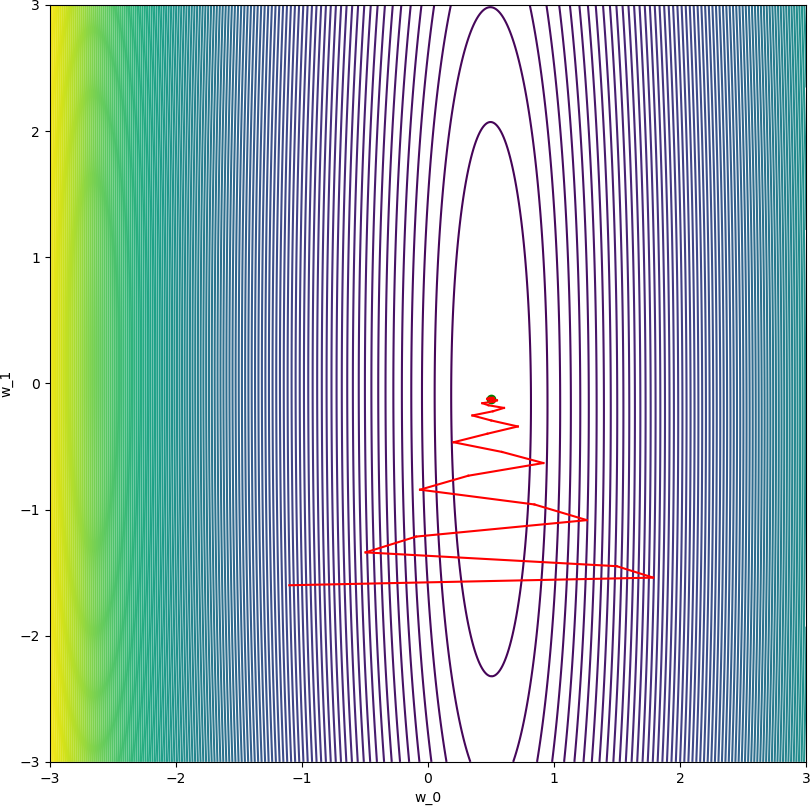
\includegraphics[width=85 mm]{images/gdm.png}
	\caption{Mô tả đường đi của thuật toán GD khi có thêm lượng quán tính trong rãnh hẹp.}
	\label{fig:gd-m}
\end{figure}

Momentum giúp giải quyết vấn đề này bằng cách sử dụng gradient tại điểm hiện tại và các giá trị gradient gần trong quá khứ. Trong rãnh hẹp được mô tả như trong hình \ref{fig:valley-momentum}, ta lấy một điểm $A$ bất kỳ. Tại đó, ta luôn có thể phân tích thành hai véc-tơ đạo hàm riêng tương ứng với từng hướng $w_1$ và $w_2$. Vì hướng $w_1$ có độ cong cao hơn hướng $w_2$ nên véc-tơ đạo hàm riêng tại hướng $w_1$ sẽ dài hơn hướng $w_2$. Ta có thể dễ dàng nhận thấy chiều véc-tơ đạo hàm riêng theo hướng $w_1$ thay đổi liên tục tại từng bước cập nhật trong khi véc-tơ đạo hàm riêng theo hướng $w_2$ ổn định qua nhiều bước liên tiếp. Sự thay đổi chiều liên tục đồng nghĩa với việc dấu của giá trị đạo hàm riêng cũng thay đổi liên tục. Do đó, khi thuật toán Momentum tíến hành cộng dồn các giá trị gradient thì các véc-tơ đạo hàm riêng thành phần tại hướng có độ dốc cao như $w_1$ sẽ bị triệt tiêu và ngược lại các véc-tơ thành phần tại các hướng như $w_2$ sẽ được tăng cường. Vì vậy, thuật toán cho phép hạn chế sự di chuyển tại hướng có dấu của gradient không ổn định và tăng cường sự di chuyển tại hướng mà dấu của gradient ổn định. Từ đó mà lượng quán tính được thêm vào trong các bước cập nhật giúp điều chỉnh hướng cập nhật và tăng tốc quá trình di chuyển trong vùng rãnh hẹp.

Đường đi của hai thuật toán GD và SGD khi có thêm quán tính chứng thực cho lý thuyết trên. Hình \ref{fig:gd-m} cho ta đường đi của thuật toán GD có thêm quán tính trong rãnh hẹp. Qua đó ta thấy được rằng đường đi ít dao động, và các bước nhảy tiến nhanh về phía cực tiểu hơn khi sử dụng thuật toán GD thuần tuý (hình \ref{fig:gd-sgd}a). Điều tương tự cũng xảy ra với thuật toán SGD. Hình \ref{fig:sgd-m} mô tả đường đi của thuật toán SGD khi có thêm lượng quán tính trong vùng rãnh hẹp. Ta có thể dễ dàng nhận ra hai giai đoạn của huấn luyện được đề cập ở phần lý thuyết. Trong giai đoạn transient, thuật toán di chuyển nhanh và không xảy ra hiện tượng dao động nhiều ở vùng rãnh hẹp. Đồng thời độ lỗi cũng giảm đáng kể sau một lần cập nhật và độ nhiễu đến từ việc gom nhóm ngẫu nhiên dữ liệu cũng được hạn chế hơn so với hình \ref{fig:gd-sgd}b. Tuy nhiên, càng về sau, khi bước qua giai đoạn finetuning, thì đường đi ngày càng nhiều dao động là minh chứng cho phần quán tính bị độ nhiễu lấn át và thuật toán suy biến về SGD thuần tuý.

\begin{figure}[htp]
	\centering
	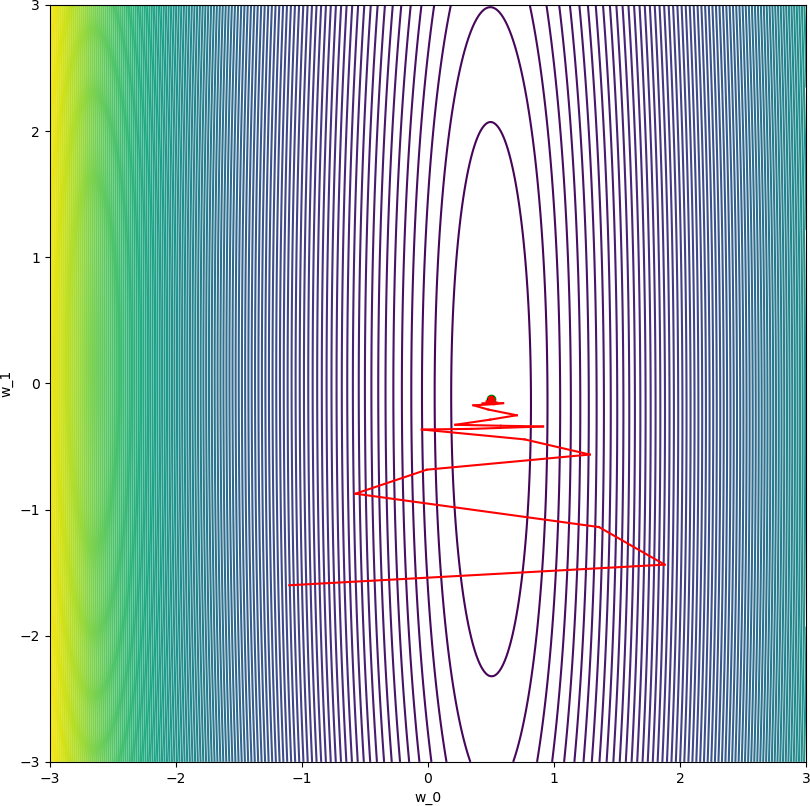
\includegraphics[width=85 mm]{images/sgdm.png}
	\caption{Mô tả đường đi của thuật toán SGD khi có thêm lượng quán tính trong rãnh hẹp.}
	\label{fig:sgd-m}
\end{figure}

Tuy nhiên, trong các vùng mà cách biệt độ lớn giữa các giá trị trọng số là rất lớn, thuật toán Momentum vẫn còn gặp những hạn chế do không có khả năng điều chỉnh tỉ lệ học thích ứng theo từng hướng. Thêm nữa, Richard S. Sutton cho rằng mặc dù thuật toán Momentum tăng tốc quá trình huấn luyện, nhưng lượng tăng tốc này vẫn còn khá nhỏ \cite{sutton1986two}. Đồng thời, bài báo cũng cho rằng để thực hiện một bước nhảy tối ưu, ta cần điều chỉnh tỷ lệ học nhỏ tại những hướng có độ cong cao và sử dụng một tỷ lệ học lớn hơn tại những hướng có độ cong thấp hơn. Đây cũng chính là ý tưởng của các phương pháp tỉ lệ học thích ứng.

\section{Thuật toán Gradient Descent với tỉ lệ học thích ứng}

Việc dự đoán trong học máy nói chung và mạng nơ-ron nhiều tầng ẩn nói riêng dựa vào quá trình trích xuất và liên hệ các đặc trưng của dữ liệu. Thông thường, các điểm dữ liệu trong cùng một bài toán sẽ có những đặc trưng chung thường gặp. Tuy nhiên, cũng có một số đặc trưng rất hiếm khi xuất hiện, chỉ có ở trong một số ít điểm dữ liệu cụ thể. Các đặc trưng hiếm gặp này thường sẽ có ảnh hưởng rất lớn về mặt ý nghĩa của dữ liệu, và mang lại rất nhiều thông tin về điểm dữ liệu đó \cite{salton1988term}. Một ví dụ cụ thể là trong phân tích văn bản, các từ xuất hiện thường xuyên như các liên từ (``và'', ``thì'', ``nhưng'',...) hay các phó từ (``cũng'', ``lại'', ``rồi'',...) lại không thể hiện nội dung nhiều bằng các danh từ và động từ chỉ các đối tượng, hành động cụ thể. Một trường hợp khác là khi xét riêng một đặc trưng, những điểm dữ liệu mang giá trị khác với các điểm dữ liệu còn lại đóng vai trò quan trọng hơn trong việc cung cấp thông tin để giải quyết bài toán.

Tuy nhiên, các thông tin quan trọng được biểu diễn bằng các đặc trưng hiếm lại ít được mạng nơ-ron nhiều tầng ẩn chú ý. Trong mạng nơ-ron nhiều tầng ẩn, các nơ-ron tương ứng với các đặc trưng thường gặp sẽ được cập nhật thường xuyên, trong khi các nơ-ron tương ứng với các đặc trưng hiếm chỉ được cập nhật một số ít lần trong một lần duyệt qua toàn tập dữ liệu. Hiện tượng này khiến cho các đặc trưng thường gặp và mang ít thông tin được biểu diễn tốt hơn, còn các đặc trưng hiếm mang nhiều ý nghĩa lại chưa được học.

Mặc dù SGD và Momentum thực hiện cập nhật một lượng khác nhau cho mỗi trọng số tùy theo độ lớn của gradient tại điểm đang xét (và trạng thái của véc-tơ quán tính tại thời điểm đó), tuy nhiên lượng cập nhật vẫn chỉ dựa vào hướng và độ dốc của gradient, hay nói cách khác là độ dốc của bề mặt lỗi, tại điểm đang xét và chưa tính tới độ nhạy cảm của các trọng số. John Duchi, Elad Hazan, và Yoram Singer đã đề xuất thuật toán Adagrad \cite{duchi2011adaptive} lấy ý tưởng từ phương pháp Newton để giải quyết vấn đề này bằng cách thích ứng lượng cập nhật cho từng trọng số: các trọng số tương ứng với các đặc trưng thường gặp sẽ được cập nhật ít hơn, còn các trọng số tương ứng với các đặc trưng hiếm sẽ được cập nhật lượng lớn hơn.

\begin{itemize}
	\item Từ khai triển Taylor ở công thức \ref{eqn:taylor-f}, chúng ta có thể tạo được một xấp xỉ bậc hai $\rho$ của hàm $f$ cho các giá trị $x$ xung quanh một điểm $x_0$:
	\begin{equation}
		\label{eqn:quad-approx}
		f(x) \approx \rho(x) = f(x_0) + f'(x_0) \cdot (x - x_0) + \frac{1}{2} \cdot f''(x_0) \cdot (x - x_0)^2
	\end{equation}
	\begin{figure}[H]
		\centering
		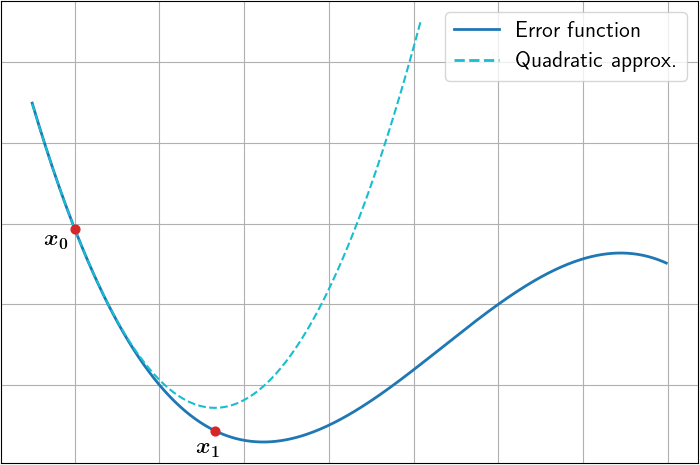
\includegraphics[width=120 mm]{images/quad-approx.png}
		\caption{Xấp xỉ bậc hai (đường đứt khúc màu xanh nhạt) của hàm lỗi (đường màu xanh đậm) và bước cập nhật tiếp theo của phương pháp Newton.}
		\label{fig:newton-step}
	\end{figure}
	Vì đây là một xấp xỉ bậc hai nên chúng ta có thể tìm cực trị của xấp xỉ này bằng cách giải phương trình $\rho '(x) = 0$. Khi đó nghiệm của $\rho'(x)$ sẽ là bước cập nhật tiếp theo của phương pháp Newton (hình~\ref{fig:newton-step}) được tính bằng công thức \ref{eqn:newton-update}:
	\begin{equation} \label{eqn:newton-update}
		\begin{aligned}
			\rho'(x_{t+1}) &= 0 \\
			\Rightarrow f'(x_t) + f''(x_t) \cdot (x_{t+1} - x_t) &= 0 \\
			\Rightarrow x_{t+1} &= x_t - \frac{f'(x_t)}{f''(x_t)}
		\end{aligned}
	\end{equation}

	\item Ma trận Hessian là ma trận vuông gồm các đạo hàm bậc hai theo từng cặp hướng của một hàm số. Cho một hàm số $f$ có tham số đầu vào là một véc-tơ $x \in \mathbb{R}^M$, chúng ta sẽ có ma trận vuông Hessian $H$ kích thước $M\times M$ theo công thức:
	\begin{equation}
		H = \begin{bmatrix}
			\frac{\delta^2 f}{\delta x^{2}_1} & \frac{\delta^2 f}{\delta x_1 \delta x_2} & \dotsb & \frac{\delta^2 f}{\delta x_1 \delta x_M} \\
			\frac{\delta^2 f}{\delta x_2 \delta x_1} & \frac{\delta^2 f}{\delta x^{2}_2} & \dotsb & \frac{\delta^2 f}{\delta x_2 \delta x_M} \\
			\vdots & \vdots & \ddots & \vdots \\
			\frac{\delta^2 f}{\delta x_M \delta x_1} & \frac{\delta^2 f}{\delta x_M \delta x_2} & \dotsb & \frac{\delta^2 f}{\delta x^{2}_M}
		\end{bmatrix}
	\end{equation}

	\item Để khái quát hóa phương pháp Newton cho bài toán tối ưu trong không gian cao chiều, ta thay đạo hàm bậc nhất và đạo hàm bậc hai từ công thức \ref{eqn:quad-approx} lần lượt bằng gradient $g(x_0)$ và ma trận Hessian $H$ tại điểm $x_0$:
	\begin{equation} \label{eqn:hessian-approx}
		f(x) \approx \rho(x) = f(x_0) + g(x_0)^\top (x - x_0) + \frac{1}{2}(x - x_0)^\top H(x - x_0)
	\end{equation}
	Tương tự như trên, chúng ta cũng giải phương trình $\nabla\rho(x)=0$ để tìm bước cập nhật tiếp theo:
	\begin{equation} \label{eqn:hessian-update}
		\begin{aligned}
			\nabla \rho(x_t) &= 0 \\
			\Rightarrow g(x_t) + H_t \cdot (x_{t+1} - x_t) &= 0 \\
			\Rightarrow x_{t+1} &= x_t - H^{-1}_t \cdot g(x_t)
		\end{aligned}
	\end{equation}
\end{itemize}

Tại mỗi bước cập nhật, phương pháp Newton xấp xỉ bề mặt lỗi xung quanh điểm hiện tại bằng một parabol $P$ có cùng độ dốc và độ cong với bề mặt lỗi tại điểm đang xét. Từ đó, bước cập nhật trong công thức \ref{eqn:hessian-update} sẽ cho một điểm mới là điểm cực trị trong parabol $P$ (cực tiểu nếu parabol $P$ có bề lõm quay lên trên; cực tiểu nếu parabol $P$ có bề lõm quay xuống dưới). Ví dụ một hàm số bậc hai có dạng $y_1 = ax^2 + bx + c$ sẽ có đồ thị là một parabol $P_1$ có bề lõm hướng lên và điểm cực tiểu là điểm $A(\frac{-b}{2a};\frac{-\Delta}{4a})$. Lấy một điểm B bất kỳ thuộc parabol $P_1$ có toạ độ $(x_B,y_B)$ với $x_B > \frac{-b}{2a}$. Để từ $B$ đến được cực tiểu $A$ trong một bước, thì toạ độ điểm $B$ phải thay đổi một lượng $\Delta x = x_B - x_A = x_B + \frac{b}{2a} = \frac{2ax_B + b}{2a} = \frac{f'(x_B)}{f''(x_B)}$. Vậy từ điểm $B$ ta thực hiện bước cập nhật $x_B - \Delta x$ thì ta đến được điểm $A$. Trong trường hợp hàm nhiều biến, đạo hàm bậc nhất $f'(x_B)$ sẽ được thay bằng véc-tơ gradient và đạo hàm bậc hai sẽ được thay bằng ma trận Hessian. Viết lại theo dạng tổng quát ta sẽ được công thức \ref{eqn:hessian-update}. Vì vậy các thuật toán bậc hai bị "thu hút" bởi các điểm cực trị dẫn đến mắc kẹt tại điểm yên ngựa. Đồng thời đây là một trong những lý do quan trọng khiến các phương pháp bậc hai ít được sử dụng hơn các phương pháp bậc nhất trong huấn luyện mạng nơ-ron nhiều tầng ẩn. Các phương pháp bậc nhất không gặp vấn đề này do hướng của gradient là hướng có độ thay đổi lớn nhất, đồng nghĩa với việc hướng gradient luôn chỉ về cực đại. Bằng cách đi ngược lại với hướng của gradient, ta luôn có thể tìm về một điểm mới có độ lỗi nhỏ hơn điểm hiện tại. Vấn đề của các phương pháp bậc nhất gặp phải là độ lớn bước cập nhật quá nhỏ. Các phương pháp tỉ lệ học thích ứng giúp thay đổi điều này bằng thông tin xấp xỉ được từ ma trận Hessian để thay đổi kích thước của bước cập nhật.

Ngoài ra, phương pháp Newton phụ thuộc khá lớn vào việc xấp xỉ cục bộ tại một điểm trên bề mặt lỗi. Vì vậy, một xấp xỉ không chính xác dễ dàng gây ra những bước cập nhật kém hiệu quả và có khả năng thuật toán không thể hội tụ tại cực tiểu. Các trường hợp này thường xảy ra khi các đạo hàm riêng bậc hai bằng 0 hoặc tiến gần về 0, khiến cho việc xấp xỉ bằng ma trận nghịch đảo không còn chính xác. Từ đó công thức \ref{eqn:hessian-update} cho ta một điểm mới có độ lỗi lớn hơn điểm hiện tại (hình \ref{fig:newton-bad-step}).

\begin{figure}
	\centering
	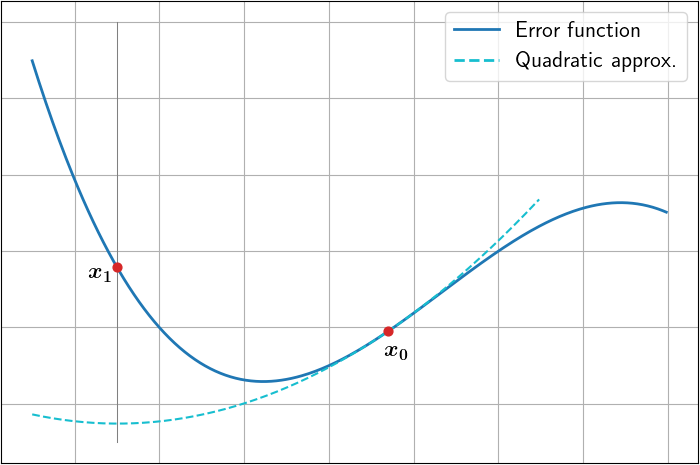
\includegraphics[width=120 mm]{images/hessian-osc.png}
	\caption{Cực tiểu của xấp xỉ bậc hai cung cấp một bước cập nhật không tối ưu.}
	\label{fig:newton-bad-step}
\end{figure}

Một hạn chế khác của các phương pháp bậc hai như phương pháp Newton nằm ở việc tính toán ma trận Hessian. Trong không gian $\mathbb{R}^M$ với $M$ có thể lên tới hàng trăm triệu hay thậm chí là hàng tỷ tương ứng với số trọng số của mô hình, ma trận Hessian sẽ yêu cầu thời gian tính toán và bộ nhớ quá lớn, dẫn đến việc sử dụng các phương pháp bậc hai cho bài toán tối ưu mạng nơ-ron nhiều tầng ẩn là bất khả thi.

Thuật toán Adagrad cũng sử dụng nguyên lý xấp xỉ bề mặt lỗi tương tự như phương pháp Newton. Tuy nhiên, thay vì tính trực tiếp ma trận Hessian nghịch đảo ($H^{-1}$, công thức \ref{eqn:hessian-update}), Adagrad chỉ thực hiện xấp xỉ tương đối $H^{-1}$ và tính bước cập nhật tiếp theo bằng công thức \ref{eqn:adagrad-base}:

\begin{equation}
	\label{eqn:adagrad-base}
	x_{t+1} = \prod^{diag(G_t)^{1/2}}_{X}(x_t-\eta\cdot diag(G_t)^{-1/2}\cdot g_t)
\end{equation}
với $g_t$ là véc-tơ gradient ở thời điểm $t$ và $G_t = \sum^{t}_{i=0}g_i\cdot g^{\top}_i$. Công thức \ref{eqn:adagrad-base} chỉ sử dụng gradient bậc nhất để xấp xỉ đường chéo của ma trận Hessian. Vì các bước tính đường chéo và căn bậc hai của ma trận $G_t$ có chi phí tuyến tính nên thuật toán Adagrad vẫn đảm bảo hiệu quả tính toán.

\begin{itemize}
	\item Vì gradient $g$ là một véc-tơ, biểu thức $g \cdot g^{\top}$ sẽ cho kết quả là một ma trận vuông kích thước $M \times M$ với mỗi phần tử là tích của từng cặp hướng trong véc-tơ gradient:
	\begin{equation} \label{eqn:grad-gradT}
		G = g \cdot g^{\top} = \begin{bmatrix}
			g^{2}_1 & g_1 \cdot g_2 & \dotsb & g_1 \cdot g_M \\ \\
			g_2 \cdot g_1 & g^{2}_2 & \dotsb & g_2 \cdot g_M \\
			\vdots & \vdots & \ddots & \vdots \\
			g_M \cdot g_1 & g_M \cdot g_2 & \dotsb & g^{2}_M
		\end{bmatrix}
	\end{equation}

	\item Từ kết quả công thức \ref{eqn:grad-gradT}, đường chéo của ma trận $G$ là véc-tơ $\begin{bmatrix} g^{2}_{1} & g^{2}_{2} & \cdots & g^{2}_{M} \end{bmatrix}$, hay bình phương của các giá trị đạo hàm riêng tại các hướng. Từ đó, ta có công thức tính $G_t$ \ref{eqn:adagrad-G} và bước cập nhật của thuật toán Adagrad được viết lại thành công thức \ref{eqn:adagrad-update}:
	\begin{equation} \label{eqn:adagrad-G}
		G_{t} = G_{t-1} + g^{2}_{t}
	\end{equation}
	\begin{equation} \label{eqn:adagrad-update}
		\theta_t = \theta_{t-1} - \frac{\eta}{\sqrt{G_t} + \epsilon} \cdot g
	\end{equation}
\end{itemize}

Tại mỗi bước cập nhật $t$, công thức \ref{eqn:adagrad-G} tính $G_t$ bằng cách cộng dồn bình phương của gradient theo từng hướng. Như vậy, các trọng số được cập nhật nhiều và thường xuyên sẽ có giá trị tương ứng trong $G_t$ lớn, trong khi các trọng số ít được cập nhật sẽ có giá trị nhỏ hơn. Do siêu tham số tỉ lệ học được chia cho căn bậc hai của $G_t$ (công thức \ref{eqn:adagrad-update}), nên tỉ lệ học của các trọng số có giá trị lớn trong $G_t$ bị tiêu giảm, đồng thời tăng cường tỉ lệ học cho các trọng số có giá trị trong $G_t$ nhỏ. Khả năng điều chỉnh tỉ lệ học tùy theo mức độ và tần suất cập nhật cho mỗi trọng số của Adagrad đã tạo ra nhóm phương pháp ``tỉ lệ học thích ứng''. Việc điều chỉnh tỉ lệ học cho từng trọng số giúp mô hình chú ý nhiều hơn đến các đặc trưng hiếm gặp của dữ liệu.

Tuy nhiên, do $g^{2}_{t}$ luôn luôn không âm nên giá trị của $G_t$ luôn luôn tăng dần, khiến cho tỉ lệ học bị giảm dần. Khi quá trình huấn luyện càng kéo dài, tỉ lệ học sẽ bị suy biến đến mức không thể thực hiện được những bước cập nhật hiệu quả. Để khắc phục vấn đề này, Tijmen Tieleman và Geoffrey Hinton đã đề xuất thuật toán RMSprop trong bài giảng trên Coursera\cite{tieleman2012rmsprop}. Thuật toán RMSprop thay đổi công thức \ref{eqn:adagrad-G}, sử dụng một tỉ lệ suy biến $\gamma$ cho $G_t$ để ưu tiên các giá trị gradient hiện tại hơn và quên dần các giá trị cũ. Bước tính $G_t$ của RMSprop trở thành công thức \ref{eqn:rmsprop-G}:

\begin{equation}
	\label{eqn:rmsprop-G}
	G_{t} = \gamma \cdot G_{t-1} + (1-\gamma) \cdot g^{2}_t
\end{equation}

Tỉ lệ suy biến $\gamma$ ưu tiên các giá trị gradient gần với hiện tại giống như hệ số $\beta$ trong thuật toán Momentum. Tuy nhiên, tỉ lệ suy biến $\gamma$ khác với $\beta$ ở chỗ nó không chỉ có tác dụng suy biến mà còn sử dụng như một hệ số tỷ lệ điều chỉnh độ lớn của bước cập nhật. Có nghĩa là nếu gán $\gamma = 0.99$ thì bên cạnh việc giá trị gradient bị suy biến thì tổng bình phương của các gradient sẽ được điều chỉnh với tỷ lệ là $\sqrt{1-\gamma} = \sqrt{1 - 0.99} = 0.1$. Như vậy, từ công thức \ref{eqn:rmsprop-G} sẽ cho bước cập nhật lớn hơn gấp 10 lần bước cập nhật của Adagrad với cùng một tỉ lệ học. Nhờ sự thay đổi này mà RMSprop có thể giữ được bước cập nhật đủ lớn khi quá trình huấn luyện kéo dài.

Công thức \ref{eqn:adagrad-base} chỉ sử dụng đường chéo trong ma trận $G$ để thực hiện xấp xỉ do đó bước cập nhật phụ thuộc vào tính độc lập của từng trọng số. Vì ta thích ứng tỉ lệ học riêng cho từng trọng số nên tính độc lập giữa các trọng số là cần thiết để đảm bảo sự thay đổi trong tỉ lệ học luôn mang lại hiệu quả tốt. Ngoài ra, ta cũng có thể xem các giá trị bình phương đạo hàm riêng của từng hướng là một hình chiếu của véc-tơ $G$ lên trục trọng số tương ứng. Do đó, độ lớn của véc-tơ hình chiếu sẽ lớn nhất nếu véc-tơ $G$ song song với trục và độ lớn sẽ ngày càng giảm khi góc hợp bởi véc-tơ G và trục trọng số tiến gần đến $90^\circ$. Từ những lý do trên mà các phương pháp tỉ lệ học thích ứng hoạt động tốt trong các trường hợp hướng nhạy cảm là hướng song song với trục trọng số.

\section{Thuật toán Adam}

Kết hợp quán tính để tăng tốc và giảm dao động của thuật toán Momentum và thích ứng tỉ lệ học cho từng trọng số của thuật toán RMSprop, ta được thuật toán Adam. Thuật toán Adam \cite{kingma2014adam} được Diederik P. Kingma và Jimmy Lei Ba công bố lần đầu tại hội nghị ICLR 2015 và được sử dụng phổ biến trong huấn luyện các mạng nơ-ron nhiều tầng ẩn.

Tương tự như thuật toán Momentum, Adam tiến hành cập nhật dựa trên trung bình chạy có trọng số của gradient để xấp xỉ trung bình của gradient hàm lỗi. Adam lưu giá trị trung bình này vào biến $m_t$ và được điều chỉnh bằng hệ số $\beta_1$. Từ đó, ta có công thức cập nhật $m_t$:

\begin{equation} \label{eqn:adam-m}
	m_t = \beta_1 \cdot m_t + (1 - \beta_1) \cdot g_t
\end{equation}

Tại mỗi bước $t$, biến $m_t$ phụ thuộc phần lớn vào giá trị của $m$ ở thời điểm từ bước cập nhật $1..t-1$. Tuy nhiên, mỗi giá trị của $m_t$ được gán với một giá trị trọng số giảm dần từ hiện tại đến quá khứ. Ngoài ra, một phần nhỏ giá trị của gradient cũng được sử dụng cập nhật biến $m_t$ nhằm cung cấp thông tin về hướng có độ giảm lớn nhất. Nhờ vậy mà Adam có thể tăng tốc trên những hướng mà dấu của gradient ổn định và hạn chế dao động tại hướng mà dấu của gradient không ổn định. Sự bất ổn định có thể đến từ việc áp dụng các biện pháp hạn chế sự overfit của mô hình, hay còn gọi là ``regularization''; việc xấp xỉ gradient trên toàn bộ tập huấn luyện dựa vào gradient của một minibatch; hoặc nó có thể do di chuyển trong địa hình rãnh hẹp với tỉ lệ học chưa đủ nhỏ.

Tuy nhiên, nếu chỉ sử dụng lượng tăng tốc đến từ biến $m_t$ thì Adam sẽ không thể vượt qua các vùng rãnh hẹp mà sự khác biệt về độ lớn của các giá trị trọng số là rất lớn và độ cong theo từng hướng là rất khác nhau. Tại các vùng này, lượng tích luỹ $m_t$ quá nhỏ để hạn chế sự di chuyển tại hướng có độ cong lớn và tăng cường sự di chuyển trên hướng có độ cong nhỏ đủ lớn để tăng tốc quá trình huấn luyện. Để giải quyết vấn đề này, ta phải thêm thông tin về độ cong của bề mặt lỗi bằng cách xấp xỉ thông qua việc sử dụng trung bình chạy của bình phương gradient. Thuật toán Adam sử dụng biến $v_t$ để lưu trữ giá trị trung bình chạy này cùng với hệ số $\beta_2$ để điều chỉnh tỉ lệ suy biến. Tương tự với $m_t$, $v_t$ cũng phụ thuộc vào các giá trị $v$ ở thời điểm trước đó và mức độ phụ thuộc giảm dần từ hiện tại tới quá khứ. Từ đó, ta có công thức cập nhật:

\begin{equation} \label{eqn:adam-v}
	v_t = \beta_2 \cdot v_t + (1 - \beta_2) \cdot g_t^2
\end{equation}

Sau đó, thuật toán Adam thực hiện thích ứng tỉ lệ học cho từng trọng số thông qua việc chia tỉ lệ học chung $\eta$ cho căn bậc hai của tích luỹ bình phương đạo hàm riêng tương ứng. Từng trọng số của mạng nơ-ron nhiều tầng ẩn được cập nhật thông qua công thức sau:

\begin{equation} \label{eqn:adam-step}
	\theta_t = \theta_{t-1} - \eta\cdot\frac{m_t}{\sqrt{v_t} + \epsilon}
\end{equation}

Kết quả là những trọng số có độ lớn đạo hàm riêng lớn trong những bước gần đây (ứng với hướng mà bề mặt lỗi có độ cong cao) thì sẽ có tỉ lệ học nhỏ; trong khi những trọng số trong lịch sử cập nhật gần nhất có độ lớn đạo hàm riêng nhỏ (ứng với hướng mà bề mặt lỗi có độ cong thấp) lại có tỉ lệ học lớn. Tuy nhiên, vì ta chỉ thực hiện cập nhật riêng lẻ cho từng trọng số nên cách làm này chỉ hoạt động tốt khi các hướng có độ cong/thấp của bề mặt lỗi song song với trục trọng số.

Đến đây, chúng ta có được thuật toán Adam được trình bày trong thuật toán \ref{alg:adam-incomplete}.

\begin{algorithm}[H]
	\caption{Adam (chưa hoàn chỉnh)} \label{alg:adam-incomplete}
	\begin{algorithmic}[1]
		\renewcommand{\algorithmicrequire}{\textbf{Đầu vào:}}
		\renewcommand{\algorithmicensure}{\textbf{Đầu ra:}}
		\algnewcommand\algorithmicoperation{\textbf{Thao tác:}}
		\algnewcommand\Operation{\item[\algorithmicoperation]}

		\Require Tập dữ liệu huấn luyện $x_i (i = 1, 2, ..., N)$, kích thước tập con $k$, tỉ lệ học $\eta$, tỉ lệ suy biến $\beta_1$ và $\beta_2$, hệ số $\epsilon$, bộ trọng số $\theta$ của mô hình $\mathcal{F}$
		\Ensure Bộ trọng số $\theta$ của $\mathcal{F}$ với độ lỗi đạt cực tiểu

		\Operation
		\State Khởi tạo $m_0=0$
		\State Khởi tạo $v_0=0$
		\State Khởi tạo $t=0$
		\While{$\theta$ chưa hội tụ}
			\State Xáo trộn tập dữ liệu.
			\For{mỗi tập con kích thước $k$}
				\State Cập nhật bước thực hiện: $t=t+1$
				\State Tính độ lỗi trung bình: $\mathbf{\it{E}(\theta)} = \frac{1}{k}\cdot \displaystyle\sum_{i=1}^{k}\mathcal{L}(\hat{y_i}, y_i)$
				\State Tính gradient của độ lỗi: $g_t =\nabla_{\theta} \mathbf{\it{E}(\theta)}$
				\State Cập nhật $m$: $m_t = \beta_1\cdot m_{t-1} + (1-\beta_1)\cdot g_t$
				\State Cập nhật $v$: $v_t = \beta_2\cdot v_{t-1} + (1-\beta_2)\cdot g^{2}_{t}$
				\State Thực hiện cập nhật trọng số: $\theta = \theta - \eta\cdot m_t/(\sqrt{v_t} + \epsilon)$
			\EndFor
		\EndWhile
		\State return $\theta$
	\end{algorithmic}
\end{algorithm}

Thông thường, các biến $m_t$ và $v_t$ sẽ được khởi tạo bằng các véc-tơ 0. Nhìn lại công thức \ref{eqn:adam-m} và \ref{eqn:adam-v}, chúng ta có thể thấy rằng với giá trị mặc định $\beta_1=0.9$ và $\beta_2=0.999$, lượng giá trị được cộng dồn vào $m_t$ và $v_t$ ở những bước đầu tiên sẽ rất nhỏ. Điều này dẫn đến hiện tượng các ước lượng bằng trung bình chạy bị ``chệch'' (bias) về 0. Hiện tượng này khiến các ước lượng này nhỏ hơn giá trị ban đầu dẫn đến các khó khăn không được khắc phục hiệu quả. Để khắc phục hệ quả này, chúng ta cần một bước ``phóng đại'' giá trị của $m_t$ và $v_t$ lên, nhờ đó khôi phục độ lớn cho các ước lượng này và không còn bị chệch về 0 nữa. Đó chính là bước bias-correction. Chúng ta thực hiện bước bias-correction này như sau:

\begin{equation} \label{eqn:adam-mvhat}
	\begin{aligned}
		\hat m_t &= \frac{m_t}{1-\beta_1^t} \\
		\hat v_t &= \frac{v_t}{1-\beta_2^t}
	\end{aligned}
\end{equation}

Tại những bước cập nhật đầu, giá trị $t$ nhỏ, ta có thể thấy sau khi điều chỉnh ta được một ước lượng $\hat m_t$ lớn hơn ban đầu gấp $1 - \beta_1^t$ lần. Vì hệ số $\beta_1$ và $\beta_2$ là các giá trị nằm trong [0;1) nên khi số lượng bước cập nhật $t$ càng lớn thì $\beta_1^t$, $\beta_2^t$ sẽ càng nhỏ và tiến dần về 0. Từ đó, công thức \ref{eqn:adam-mvhat} sẽ cho ước lượng $m_t$ ban đầu bằng với ước lượng $\hat m_t$ lúc sau và tương tự với ước lượng $v_t$ và $\hat v_t$.

Cuối cùng, chúng ta có thuật toán Adam đầy đủ, được trình bày chi tiết trong thuật toán \ref{alg:adam-complete}.

\begin{algorithm}
	\caption{Adam} \label{alg:adam-complete}
	\begin{algorithmic}[1]
		\renewcommand{\algorithmicrequire}{\textbf{Đầu vào:}}
		\renewcommand{\algorithmicensure}{\textbf{Đầu ra:}}
		\algnewcommand\algorithmicoperation{\textbf{Thao tác:}}
		\algnewcommand\Operation{\item[\algorithmicoperation]}

		\Require Tập dữ liệu huấn luyện $x_i (i = 1, 2, ..., N)$, kích thước tập con $k$, tỉ lệ học $\eta$, tỉ lệ suy biến $\beta_1$ và $\beta_2$, hệ số $\epsilon$, bộ trọng số $\theta$ của mô hình $\mathcal{F}$
		\Ensure Bộ trọng số $\theta$ của $\mathcal{F}$ với độ lỗi đạt cực tiểu

		\Operation
		\State Khởi tạo $m_0=0$
		\State Khởi tạo $v_0=0$
		\State Khởi tạo $t=0$
		\While{$\theta$ chưa hội tụ}
			\State Xáo trộn tập dữ liệu.
			\For{mỗi tập con kích thước $k$}
				\State Cập nhật bước thực hiện: $t=t+1$
				\State Tính độ lỗi trung bình: $\mathbf{\it{E}(\theta)} = \frac{1}{k}\cdot \displaystyle\sum_{i=1}^{k}\mathcal{L}(\hat{y_i}, y_i)$
				\State Tính gradient của độ lỗi: $g_t =\nabla_{\theta} \mathbf{\it{E}(\theta)}$
				\State Cập nhật $m$: $m_t = \beta_1\cdot m_{t-1} + (1-\beta_1)\cdot g_t$
				\State Cập nhật $v$: $v_t = \beta_2\cdot v_{t-1} + (1-\beta_2)\cdot g^{2}_{t}$
				\State Thực hiện cập nhật trọng số: $\theta = \theta - \eta\cdot m_t/(\sqrt{v_t} + \epsilon)$
			\EndFor
		\EndWhile
		\State return $\theta$
	\end{algorithmic}
\end{algorithm}

\chapter{Các kết quả thí nghiệm}
\label{Chapter4}

\textit{Trong chương này, chúng tôi tiến hành các thí nghiệm nhằm kiểm chứng lý thuyết về thuật toán Adam đã trình bày ở chương 3. Trước hết, để so sánh kết quả cài đặt của chúng tôi với kết quả được công bố trong bài báo gốc, chúng tôi thí nghiệm huấn luyên mạng “Multi-layer Neural Network” trên bộ dữ liệu ảnh nhỏ là MNIST và mạng "Convolutional Neural Network" trên bộ dữ liệu ảnh trung là CIFAR10. Tiếp theo, chúng tôi thực hiện thí nghiệm trực quan hóa cách Adam và các thuật toán khác di chuyển trong trường hợp bề mặt lỗi có dạng rãnh hẹp và rãnh rất hẹp; dữ liệu được sử dụng trong thí nghiệm này là dữ liệu tự tạo và ít chiều để có thể trực quan hóa. Cuối cùng, để thấy rõ hơn về hiệu quả của Adam so với các thuật toán khác trong ngữ cảnh thực tế, chúng tôi thí nghiệm huấn luyện mạng "Convolutional Neural Network" trên bộ dữ liệu ảnh lớn là ImageNet và mạng "Long Short-term Memory" trên bộ ngữ liệu là Penn Treebank.}

\section{Các thiết lập thí nghiệm}

Chúng tôi thực hiện hai loại thí nghiệm: thí nghiệm nguyên lý và thí nghiệm thực tế. Trong các thí nghiệm nguyên lý, chúng tôi sử dụng hàm số để tạo ra dạng địa hình bề mặt lỗi mong muốn. Ngoài ra, chúng tôi cũng tạo một bộ dữ liệu ngẫu nhiên cho các thí nghiệm sử dụng minibatch. Với các thí nghiệm thực tế, chúng tôi sử dụng nhiều bộ dữ liệu khác nhau cùng với các kiến trúc mạng nơ-ron nhiều tầng ẩn được sử dụng để giải quyết các bài toán ứng dụng hiện nay. Những bộ dữ liệu thực tế mà chúng tôi sử dụng:

\begin{itemize}
	\item MNIST \cite{lecun2010mnist}: Bộ dữ liệu này gồm các ảnh xám của các chữ số viết tay từ 0 đến 9 có kích thước 28x28. Tập dữ liệu gồm 60000 ảnh huấn luyện và 10000 ảnh kiểm tra.
	\item CIFAR10 \cite{krizhevsky2009cifar10}: Bộ dữ liệu này gồm các ảnh màu của 10 lớp đối tượng có kích thước 32x32. Tập dữ liệu có tổng cộng 60000 ảnh, mỗi lớp đối tượng có 6000 ảnh. Trong đó 50000 ảnh được chọn làm ảnh huấn luyện và 10000 ảnh kiểm tra. Bộ dữ liệu này và MNIST là những bộ dữ liệu cơ bản phổ biến để huấn luyện các thuật toán học máy và mạng nơ-ron nhiều tẩng ẩn đơn giản.
	\item ImageNet \cite{deng2009imagenet}: Đây là một trong những bộ dữ liệu hình ảnh lớn nhất hiện nay, thường được dùng để kiểm tra khả năng của các phương pháp thị giác máy tính mới nhất. Phiên bản của bộ dữ liệu mà chúng tôi sử dụng là phiên bản được sử dụng trong thử thách ImageNet Large Scale Visual Recogition Challenge 2012 (ILSVRC2012), với hơn 1.2 triệu ảnh được gán nhãn vào 1000 lớp đối tượng được sử dụng để huấn luyện, và 50000 ảnh để kiểm thử.
	\item Penn Treebank \cite{marcus1993ptb}: Đây là bộ dữ liệu do Marcus và cộng sự tổng hợp gồm 929 000 từ dùng để huấn luyện, 73 000 từ cho tập kiểm thử và 82 000 từ để kiểm tra. Tập dữ liệu gồm có 10 000 từ trong tập từ điển. Tập dữ liệu đã được qua xử lý được lấy từ trang web của Tomas Mikolov (\url{http://www.fit.vutbr.cz/~imikolov/rnnlm/simple-examples.tgz}).
\end{itemize}

Chúng tôi sử dụng ngôn ngữ lập trình Python và thư viện Numpy cho các thí nghiệm nguyên lý, thư viện Pytorch cho các thí nghiệm thực tế. Cả thư viện Numpy và Pytorch đều cung cấp khả năng tăng tốc thực thi bằng việc véc-tơ hóa tính toán trên nền C/C++. Thư viện Numpy tập trung vào các chức năng tính toán đại số trên CPU, phù hợp với các thí nghiệm đơn giản; trong khi thư viện Pytorch là một thư viện máy học có thể xây dựng các mạng nơ-ron nhiều tầng ẩn phức tạp cùng với khả năng thực thi song song trên GPU. Loại GPU mà chúng tôi sử dụng là NVIDIA RTX 2080, ngoài ra chúng tôi cũng sử dụng NVIDIA Tesla T4 và TPU (Tensor Processing Unit) trên nền tảng Google Cloud.

Trong tất cả các thí nghiệm, tất cả các thuật toán tối ưu đều có chung điểm xuất phát: bộ trọng số ban đầu đầu của mạng nơ-ron nhiều tầng ẩn sau khi khởi tạo ngẫu nhiên lần đầu sẽ được lưu lại; và với mỗi thuật toán tối ưu được thử nghiệm, bộ trọng số này sẽ được nạp lại vào mạng nơ-ron rồi từ đó mới bắt đầu tiến hành tối ưu và ghi nhận lại kết quả. Điều này giúp đảm bảo sự công bằng cho tất cả các thuật toán khi tiến hành thử nghiệm, tránh được trường hợp một thuật toán nào đó "may mắn" được bắt đầu ở một điểm thuận lợi hơn và nhờ vậy mà hội tụ nhanh hơn.

\begin{center}
	\begin{table}
		\begin{tabularx}{\textwidth}{{|l|l|X|X|}}
			\hline
			\textbf{Thuật toán} & \textbf{Tỉ lệ học} & \textbf{Momentum/$\beta_1$} & \textbf{Alpha/$\beta_2$} \\
			\hline
			SGD & [0.0001, 1] & - & - \\
			\hline
			Momentum & [0.0001, 0.1] & [0.1, 0.99] & - \\
			\hline
			Adagrad & [0.0001, 0.1] & - & - \\
			\hline
			RMSprop & [0.0001, 0.1] & - & [0.9, 0.999] \\
			\hline
			Adam & [0.0001, 0.1] & [0.1, 0.99] & [0.9, 0.999] \\
			\hline
		\end{tabularx}
	\caption{\label{tab:hparam-search}Khoảng giá trị để dò tìm siêu tham số tốt nhất của các thuật toán tối ưu.}
	\end{table}
\end{center}

\section{Các kết quả thí nghiệm}

\subsection{Kết quả của thuật toán cài đặt so với bài báo}
\label{exp:replicate}

Trong phần này, chúng tôi trình bày kết quả của các thuật toán tối ưu mà chúng tôi cài đặt. Cụ thể, chúng tôi so sánh kết quả của các thuật toán do chúng tôi cài đặt lại trên nền thư viện Pytorch với kết quả được công bố trong bài báo thí nghiệm ``Multi-layer Neural Network'' trên tập dữ liệu MNIST và thí nghiệm ``Convolutional Neural Network'' trên tập dữ liệu CIFAR10. Việc tái tạo các kết quả được công bố gặp nhiều khó khăn do bản chất ngẫu nhiên của SGD và dropout, cộng với việc tác giả không công bố các siêu tham số cho các thí nghiệm cũng như các cài đặt liên quan khác. Bài báo cũng không đề cập các khoảng tìm kiếm cho quá trình tìm siêu tham số tối ưu nhất của mỗi thuật toán, vì vậy chúng tôi đã tham khảo các công trình nghiên cứu khác sử dụng các tối ưu này, và tổng hợp các giá trị nhỏ nhất và lớn nhất cho từng siêu tham số của mỗi thuật toán để làm khoảng tìm kiếm (bảng \ref{tab:hparam-search}). Bài báo thực hiện thí nghiệm với thuật toán Nesterov \cite{nesterov1983amf}, Adagrad, RMSprop, AdaDelta \cite{zeiler2012adadelta} và Adam; tuy nhiên chúng tôi nhận thấy rằng Nesterov và AdaDelta không liên quan trực tiếp đến thuật toán Adam mà khóa luận tập trung tìm hiểu, vì vậy chúng tôi sẽ tập trung thực hiện thí nghiệm trên các thuật toán SGD, Momentum, Adagrad, RMSprop, và Adam.

Trong thí nghiệm Multi-layer Neural Network, kết quả mà chúng tôi cài đặt so với kết quả được công bố trong bài báo xấp xỉ nhau về đường đi và vị trí tương đối giữa các thuật toán với nhau (hình \ref{fig:exp-mlp}). Tuy nhiên, giá trị độ lỗi trong cài đặt của chúng tôi cũng thấp hơn đáng kể so với kết quả trong bài báo.

\begin{figure}[htp]
	\centering
	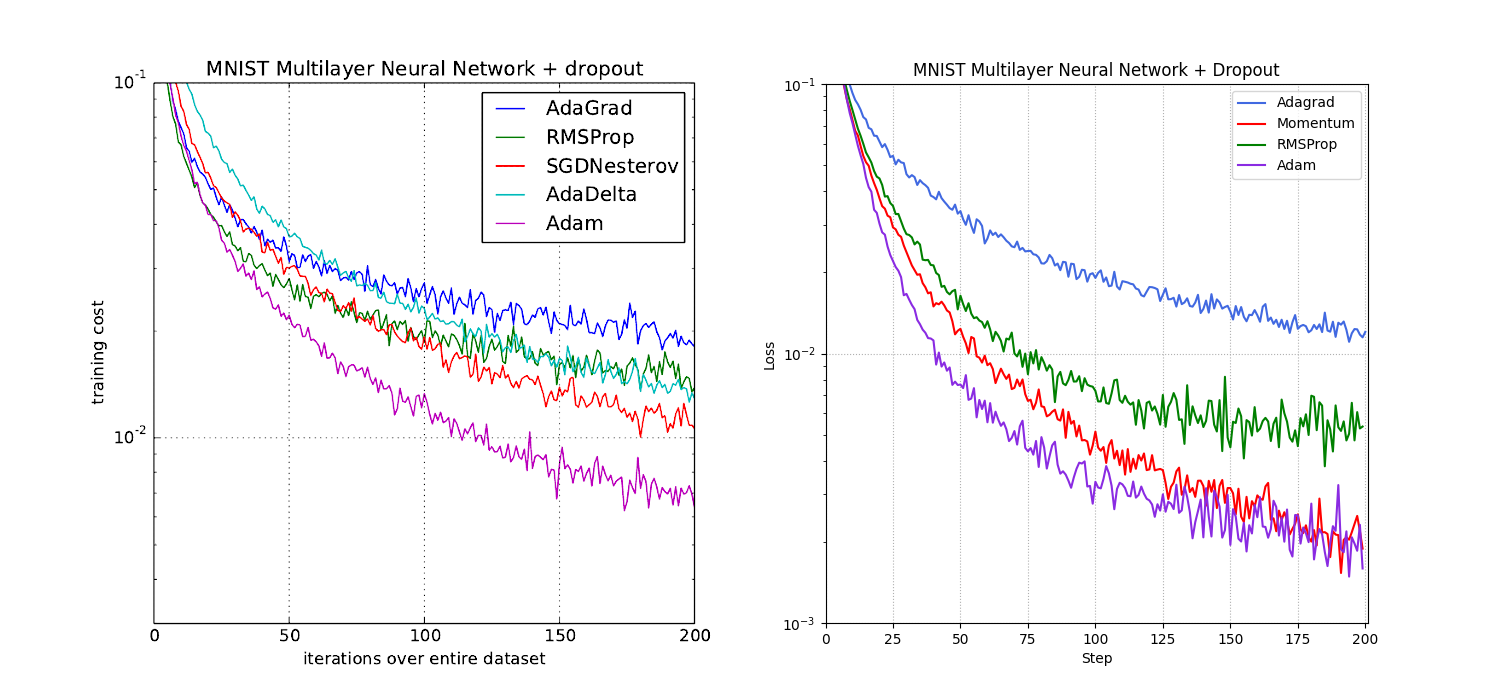
\includegraphics[width=160 mm]{images/mlp.png}
	\caption{Kết quả thí nghiệm Multi-layer Neural Network giữa thuật toán mà chúng tôi cài đặt so với bài báo. Bên trái: kết quả mà bài báo công bố. Bên phải: kết quả do chúng tôi tự cài đặt lại.}
	\label{fig:exp-mlp}
\end{figure}

Nhìn chung, thuật toán Adam có tốc độ tối ưu độ lỗi nhanh nhất trong tất cả các thuật toán được thử nghiệm. Điểm yếu của Adagrad về tỉ lệ học luôn giảm dần được thể hiện rõ khi Adagrad chuyển hướng đi ngang dần mặc dù độ lỗi vẫn cao trong khi các thuật toán khác tiếp tục đi xuống. Điều đó cho thấy rằng mô hình vẫn đang trong quá trình học dữ liệu, nhưng vì tỉ lệ học quá nhỏ nên ở mỗi bước, lượng cập nhật trọng số không đủ để cải thiện mô hình. Vấn đề tỉ lệ học giảm dần do cộng dồn gradient bình phương của Adagrad được RMSprop khắc phục bằng một tỉ lệ suy biến, giúp RMSprop bắt kịp gần hơn với Momentum và Adam. Sự chênh lệch lớn nhất giữa các kết quả nằm ở 2 thuật toán Momentum và Nesterov. Mặc dù 2 thuật toán này chỉ có một sự khác nhau nhỏ ở cách mà quán tính được sử dụng, với Nesterov là phiên bản cố gắng cải thiện hướng cập nhật cho Momentum, tuy nhiên kết quả lại cho thấy Momentum có kết quả tốt hơn khi đạt được độ lỗi thấp hơn RMSprop và ngang bằng với Adam ở các bước cuối cùng.

Trong thí nghiệm Convolutional Neural Network, chúng tôi cũng thực hiện tìm bộ siêu tham số đem lại kết quả cuối cùng thấp nhất cho mỗi thuật toán. Tuy nhiên, sau khi đã tìm được những bộ siêu tham số cho tất cả các thuật toán và thực hiện thí nghiệm, chúng tôi thấy được rằng hầu hết các thuật toán trong cài đặt của chúng tôi đều giúp mô hình đạt được độ lỗi thấp hơn đáng kể so với bài báo khi không dùng dropout. Các giá trị siêu tham số được sử dụng được trình bày chi tiết trong bảng \ref{tab:cnn-hparam}.

Từ hình \ref{fig:exp-cnn-best}, chúng ta có thể thấy rằng bề mặt lỗi của thí nghiệm này có một đoạn dốc xuống khá rõ rệt, và các thuật toán SGD, Momentum cũng như Adam đều giảm độ lỗi rất nhanh khi tìm thấy đoạn dốc ấy. Trong bài báo gốc, một số thuật toán tìm thấy đoạn dốc này ngay từ những epoch đầu tiên, trong khi cài đặt của chúng tôi chỉ bắt đầu giảm mạnh từ khoảng epoch thứ 15. Trong kết quả của chúng tôi, SGD là thuật toán đầu tiên tìm ra đoạn dốc, nhưng độ lỗi tại epoch cuối lại hơi cao hơn so với Momentum và Adam. Có thể là do SGD bị giới hạn bởi tỉ lệ học trong khi hai thuật toán kia có cơ chế tăng tốc giúp đạt được độ lỗi thấp. Kết quả độ lỗi và thời gian thực thi được trình bày trong bảng \ref{tab:cnn-results}.

\begin{figure}[H]
	\centering
	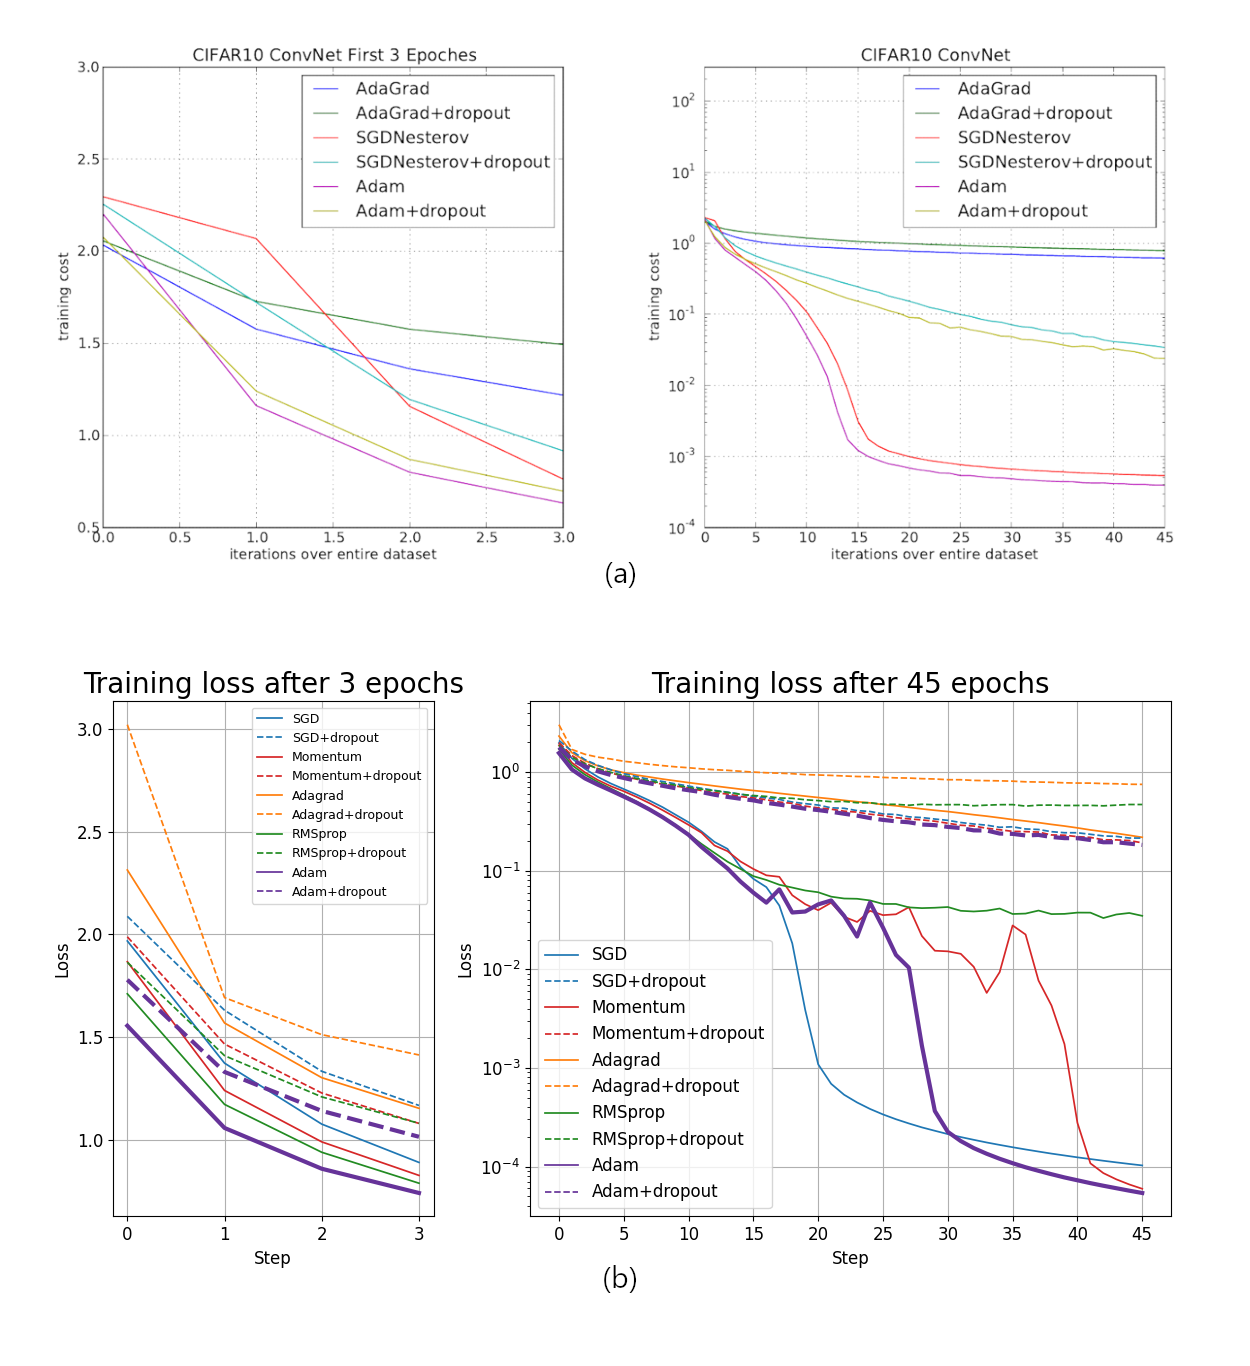
\includegraphics[width=140 mm]{images/cnn.png}
	\caption{Kết quả thí nghiệm Convolutional Neural Network giữa thuật toán mà chúng tôi cài đặt so với bài báo. (a): kết quả mà bài báo công bố. (b): kết quả do chúng tôi tự cài đặt lại.}
	\label{fig:exp-cnn-best}
\end{figure}

\begin{table}
	\begin{tabular}{|m{0.3\textwidth}|>{\raggedright\arraybackslash}m{0.33\textwidth}|m{0.3\textwidth}|}
		\hline
		\textbf{Thuật toán} & \textbf{Thời gian thực hiện (giây)} & \textbf{Độ lỗi thấp~nhất} \\
		\hline
		SGD              & \textbf{6.02 $\pm$ 0.07} & 0.0001 \\
		SGD+dropout      & \textbf{6.04 $\pm$ 0.07} & 0.2139 \\
		\hline
		Momentum         & 6.10 $\pm$ 0.07          & 0.00006 \\
		Momentum+dropout & 6.08 $\pm$ 0.07          & 0.1914 \\
		\hline
		Adagrad          & 6.14 $\pm$ 0.09          & 0.2178 \\
		Adagrad+dropout  & 6.16 $\pm$ 0.09          & 0.7496 \\
		\hline
		RMSprop          & 6.16 $\pm$ 0.07          & 0.03307 \\
		RMSprop+dropout  & 6.19 $\pm$ 0.07          & 0.4512 \\
		\hline
		Adam             & 6.19 $\pm$ 0.07          & \textbf{0.000054} \\
		Adam+dropout     & 6.23 $\pm$ 0.07          & \textbf{0.1824} \\
		\hline
	\end{tabular}
\caption{\label{tab:cnn-results}Kết quả và thời gian thực hiện một epoch của các thuật toán trong thí nghiệm Convolutional Neural Network.}
\end{table}

Về mặt thời gian tính toán, bảng \ref{tab:cnn-results} cho thấy với cùng một kích thước minibatch, có thể dễ hiểu khi SGD cho thời gian tính toán nhanh nhất vì thuật toán này chỉ tính gradient và cập nhật trọng số. Với Momentum, bước tính véc-tơ quán tính $v_t$ trước khi cập nhật trọng số làm tăng thời gian thực hiện mỗi epoch thêm khoảng 15$\%$. Bước tính đường chéo ma trận $G_t$ của các thuật toán tỉ lệ học thích ứng tốn nhiều thời gian hơn đáng kể, vì trong bước này còn có thao tác bình phương các phần tử trong véc-tơ gradient trước khi cộng dồn (thuật toán RMSprop có thêm bước nhân các phần tử này với hệ số suy biến). Adam kết hợp các bước tính quán tính trong Momentum và thích ứng tỉ lệ học, vì vậy Adam có thời gian thực thi chậm nhất trong tất cả các thuật toán.

Ngoài việc tìm bộ siêu tham số cho kết quả tốt nhất, chúng tôi cũng cố gắng tái tạo kết quả mà bài báo đã công bố. Chúng tôi thực hiện quá trình tái tạo này để kiểm tra tính khả thi của các kết quả mà bài báo đã công bố (phụ lục \ref{Appendix2}). Nhìn chung, chúng tôi có thể tái tạo các kết quả thí nghiệm mà bài báo công bố. Tuy nhiên, các kết quả tốt nhất của chúng tôi có độ lỗi thấp hơn đáng kể so với bài báo, đặc biệt là trong thí nghiệm Convolutional Neural Network. Vì không biết chính xác quá trình cài đặt và các siêu tham số đã được sử dụng trong bài báo gốc nên chúng tôi không thể khẳng định nguyên nhân của sự chênh lệch này.

\subsection{So sánh Adam với các thuật toán khác trong trường hợp bề mặt lỗi có dạng rãnh hẹp}

\subsubsection{Rãnh hẹp với các hướng có độ cong khác nhau trùng với trục trọng số}
\label{exp:step-size}

Trong thí nghiệm này, chúng tôi kiểm chứng các khó khăn của dạng địa hình rãnh hẹp và cách các thuật toán khác nhau di chuyển trong đó. Vùng rãnh hẹp là vùng mà độ cong giữa các chiều có sự chênh lệch rất lớn. Cụ thể hơn, một số hướng sẽ có độ cong rất lớn trong khi các hướng khác lại rất bằng phẳng. Vì vậy, để có thể di chuyển hiệu quả trong địa hình này, chúng ta cần giảm kích thước bước cập nhật trên các chiều có độ cong lớn để tránh hiện tượng dao động, đồng thời cập nhật những bước dài hơn trên các chiều bằng phẳng có giá trị gradient nhỏ.

Chúng tôi sử dụng một hàm lỗi giả lập có 2 tham số với sự chênh lệch độ cong trên mỗi trục là rất lớn để tạo thành rãnh hẹp. Gradient của hàm mục tiêu tại vị trí đang xét mà các thuật toán sử dụng có thể được coi như gradient của cả tập dữ liệu. Tất cả các thuật toán đều có cùng một điểm xuất phát.

\begin{figure}[htp]
	\centering
	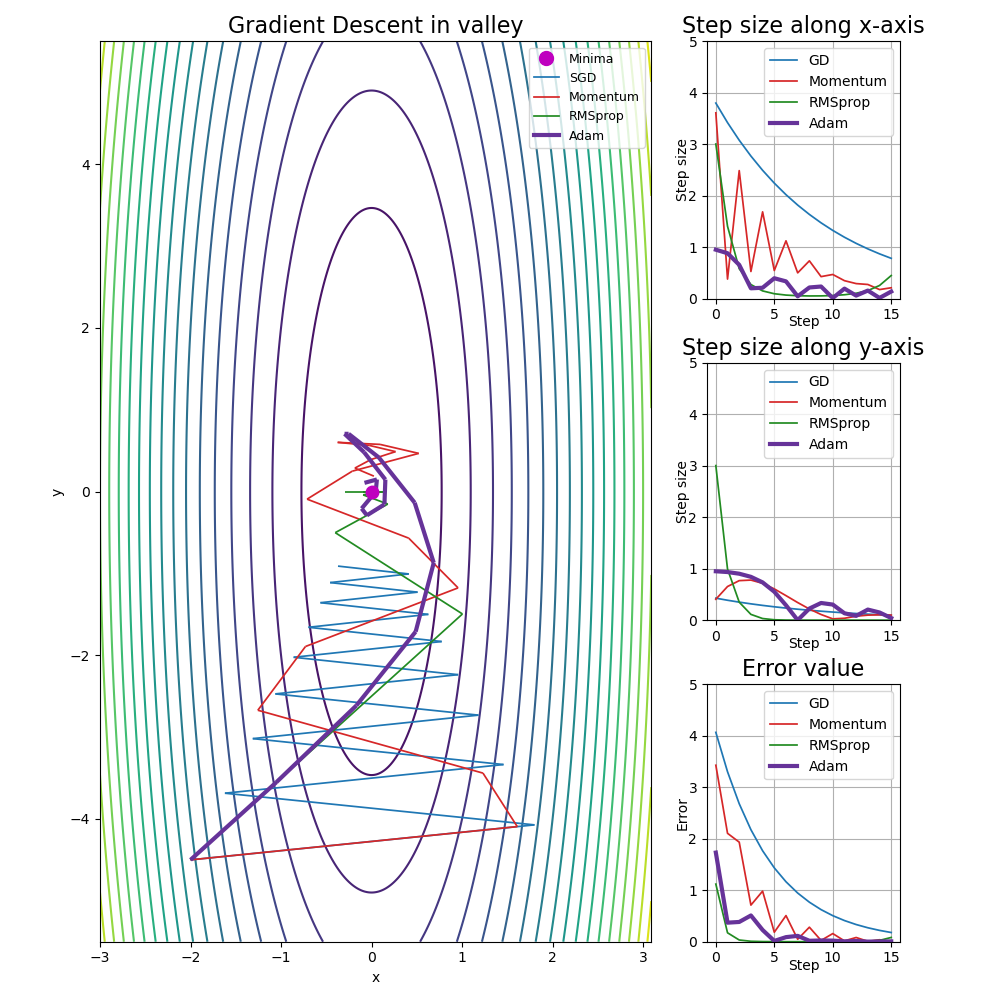
\includegraphics[width=140 mm]{images/step-size.png}
	\caption{Đường đi, độ lớn bước cập nhật theo từng chiều, và độ lỗi của các thuật toán trong quá trình tối ưu hàm giả lập.}
	\label{fig:aligned-step-size}
\end{figure}

Phân tích kết quả chạy thí nghiệm ở hình \ref{fig:aligned-step-size}, ta thấy Adam là thuật toán tối ưu độ lớn bước cập nhật trên cả trục $x$ và trục $y$ tốt nhất. Ta thấy rằng, trong khi các thuật toán khác có độ lớn bước cập nhật đầu khá lớn (RMSProp là 3 ở cả hai trục) hoặc rất khác nhau (Momentum có độ lớn trên trục $x$ lớn hơn trên trục $y$ gấp gần 4 lần), Adam giữ độ lớn của bước cập nhật đầu tiên khá gần nhau và ở giá trị nhỏ (độ lớn bước cập nhật trên cả hai trục là xấp xỉ nhau và gần bằng 1).

Adam giúp giảm dao động tốt hơn Momentum. Trên trục có độ dốc cao $x$, mặc dù độ lớn bước cập nhật của Adam và Momentum đều giảm dần khi tiến càng gần về cực tiểu nhưng Adam cho biên độ dao động nhỏ hơn Momentum rất nhiều thể hiện Adam hạn chế dao động tốt hơn Momentum. Ngược lại trên trục có độ dốc thấp $y$, Adam tăng cường bước cập nhật hiệu quả hơn Momentum khi biên độ dao động độ lớn bước cập nhật của Adam lớn hơn Momentum.

Sự dao động trên cả hai trục cũng giúp cho Adam hoạt động tốt hơn RMSprop với độ lớn bước cập nhật giảm dần ở cả hai trục. Ngoài ra, Adam còn khắc phục nhược điểm gây ra do xấp xỉ bậc hai ở vùng gần cực tiểu tốt hơn RMSprop. Điều này được thể hiện ở các bước cập nhật cuối trên trục có độ dốc cao, RMSprop cho bước cập nhật cuối lớn hơn đáng kể các thuật toán như Adam và Momentum. Đó là lý do vì sao Adam có độ lỗi thấp hơn RMSprop mặc dù đường đi của Adam đi lố qua cực tiểu nhiều hơn RMSprop.

\subsubsection{Rãnh hẹp với các hướng có độ cong khác nhau không trùng với các trục trọng số}
\label{exp:aligned-nonaligned}

Từ nội dung đã trình bày ở chương \ref{Chapter3}, các thuật toán tỉ lệ học thích ứng thay đổi tỉ lệ học theo từng trọng số riêng biệt. Vì vậy, dạng địa hình rãnh hẹp có các hướng trùng với trục của trọng số sẽ là trường hợp mà các thuật toán tỉ lệ học thích ứng phát huy hiệu quả cao nhất. Ngược lại, trường hợp rãnh hẹp chéo góc so với các trục của trọng số sẽ gây ra nhiều khó khăn nhất cho các thuật toán ấy.

Trong thí nghiệm này, thay vì tối ưu trực tiếp trên hàm giả lập, chúng tôi tạo một bộ dữ liệu ngẫu nhiên gồm 10000 phần tử có phân phối đều trên một trục, với giá trị của các điểm dữ liệu trên trục còn lại được quyết định bởi một hàm có 2 tham số. Cách thiết lập này giúp đạt được 2 mục đích: (1) xuất hiện địa hình rãnh hẹp thông qua điều chỉnh mức độ chênh lệch giữa 2 tham số; (2) chiều của rãnh hẹp không còn trùng với tham số. Chúng tôi thực hiện ``fit'' một đường thẳng hồi quy trên bộ dữ liệu này bằng phương pháp Stochastic Gradient Descent. Kích thước minibatch mà chúng tôi sử dụng là 50.

\begin{figure}[htp]
	\centering
	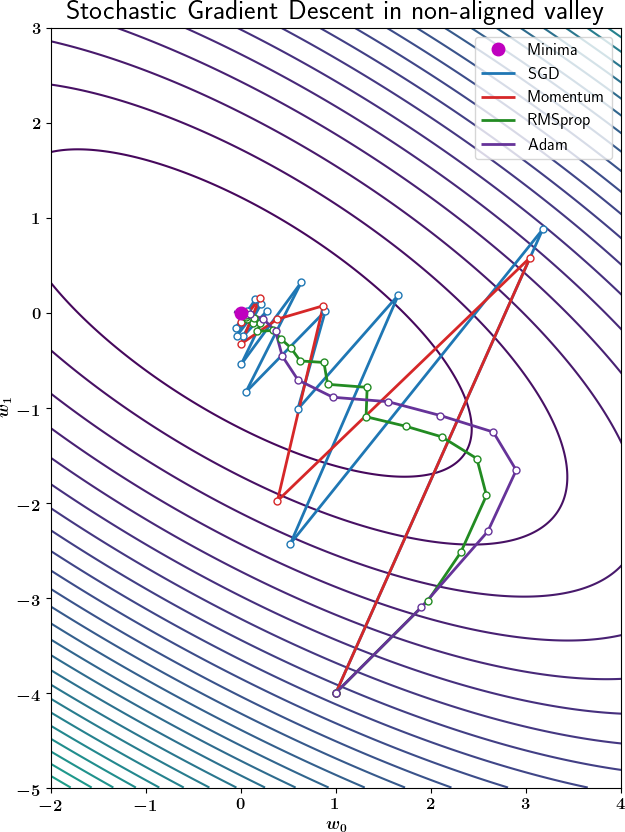
\includegraphics[width=100 mm]{images/nonaligned.png}
	\caption{Đường đi của các thuật toán trong rãnh hẹp có hướng không trùng với trọng số (b).}
	\label{fig:aligned-nonaligned}
\end{figure}

Trong trường hợp các hướng của rãnh hẹp không trùng với trục của trọng số (hình \ref{fig:aligned-nonaligned}b), thuật toán Adam không còn hiệu quả như khi trùng với trục trọng số. Mặc dù Adam vẫn cho biên độ dao động nhỏ hơn Momentum theo hướng có độ dốc cao nhưng độ lớn bước cập nhật trên hướng có độ dốc thấp đã không còn lớn như trường hợp rãnh hẹp trùng với trục trọng số. Tuy nhiên, nhờ sử dụng thêm quán tính mà Adam vẫn giữ được kích thước bước cập nhật lớn hơn RMSprop càng về sau của quá trình huấn luyện; đồng thời Adam điều chỉnh hướng đi tốt hơn và có thể triệu tiêu hiện tượng ``zig zag'' của RMSprop. Từ thí nghiệm cho thấy, vì Adam kết hợp sử dụng quán tính với tỉ lệ học thích ứng nên thuật toán vẫn có thể hoạt động tốt trong trường hợp rãnh hẹp không trùng với trục của trọng số. Điều này cho thấy Adam phù hợp với nhiều dạng địa hình khác nhau trong bề mặt lỗi.

\subsection{So sánh Adam với các thuật toán khác trong trường hợp bề mặt lỗi có dạng rãnh rất hẹp}
\label{exp:sparse-noisy}

Đặc trưng thưa là những đặc trưng mang giá trị 0 hoặc gần bằng 0 tại đa số các điểm dữ liệu; ngược lại, ta có đặc trưng đặc. Số lần các đặc trưng thưa được cập nhật là rất ít hoặc cập nhật với lượng rất nhỏ, từ đó kéo dài quá trình huấn luyện mạng nơ-ron nhiều tầng ẩn. Thêm nữa, đặc trưng thưa xuất hiện ở hầu hết các bài toán ứng dụng mạng nơ-ron sâu hiện nay nên đây là vấn đề cần được giải quyết.

Để quan sát cách các thuật toán tối ưu hoạt động với dữ liệu thưa, thí nghiệm sử dụng dữ liệu là $n$ cặp $(x,y)$, với $n = 1000$ được khởi tạo ngẫu nhiên. Sau đó, chọn $90\%$ trong số $n$ cặp và gán giá trị $x = 0$ với mục đích là khiến cho đặc trưng $x$ thưa. Sử dụng hàm mục tiêu có dạng $y = wx + b$, các thuật toán được sử dụng để tối ưu hàm chi phí $MSE = \frac{1}{n}\sum_{i=1}^n(y - wx - b)^2$. Kết quả độ lỗi sau 20 epoch với kích thước minibatch bằng 100 được thể hiện như trong hình \ref{fig:sparse}b và hình \ref{fig:sparse}a thể hiện đường đi của các thuật toán trên bề mặt lỗi. Vì đặc trưng có giá trị gần bằng 0 chiếm đa số nên hướng tương ứng của đặc trưng đó trên mặt phẳng lỗi là một vùng có độ cong thấp cho độ lỗi các hướng gần bằng nhau. Kết hợp với hướng $b$ ứng với đặc trưng đặc có độ cong cao, bề mặt lỗi trong trường hợp này hình thành một rãnh rất hẹp do sự khác nhau giữa hai hướng là rất lớn.

\begin{figure}[htp]
	\centering
	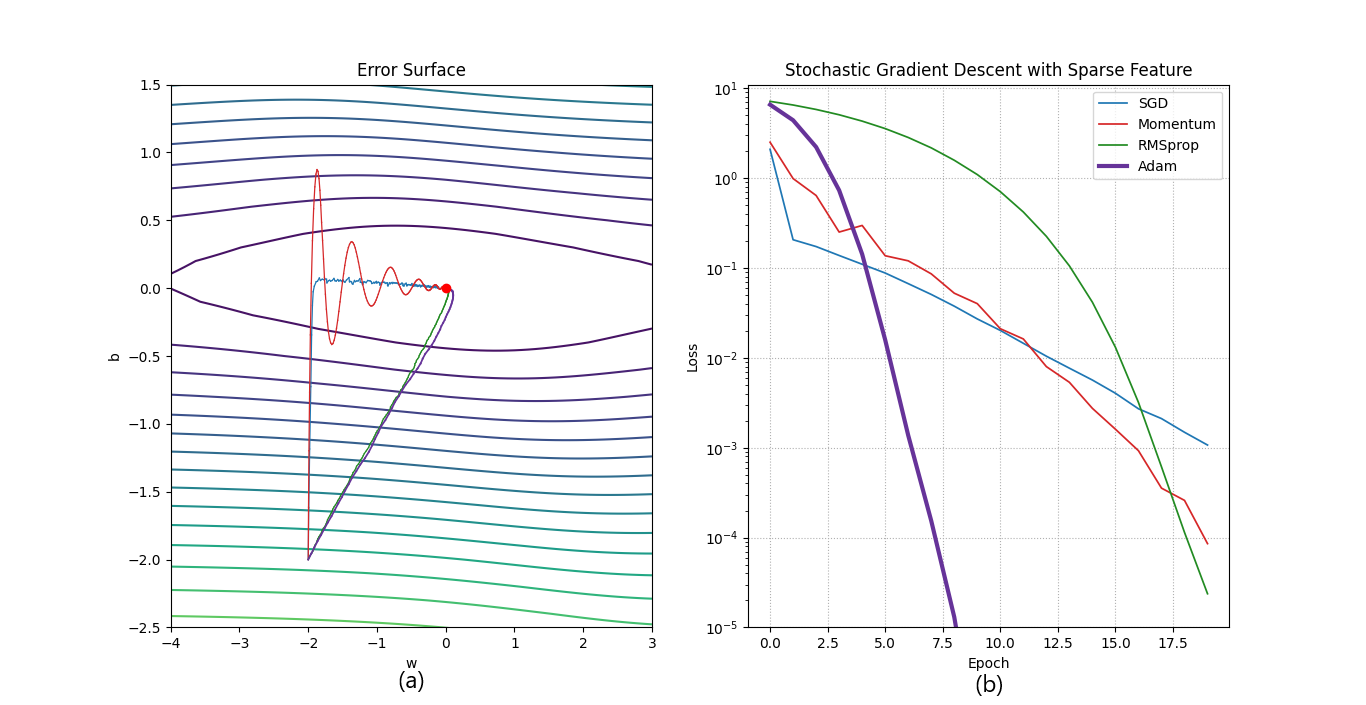
\includegraphics[width=130 mm]{images/sparse.png}
	\caption{Đường đi của các thuật toán trong bề mặt lỗi (a) và độ lỗi (b) của từng thuật toán trong trường hợp đặc trưng thưa.}
	\label{fig:sparse}
\end{figure}

Nhìn chung, thí nghiệm cho thấy thuật toán Adam là thuật toán hoạt động tốt nhất (cả về mặt độ lỗi lẫn thời gian huấn luyện) trong trường hợp bề mặt lỗi có dạng rãnh rất hẹp. Trong trường hợp này, một hệ số quán tính lớn cũng không đem lại nhiều lợi ích cho việc di chuyển theo hướng có độ cong thấp vì sẽ dẫn đến dao động cao trên hướng có độ cong cao và gần cực tiểu nên Momentum chỉ có thể di chuyển chậm theo hướng w. Vì cơ chế của tỉ lệ học thích ứng nên Adam và RMSprop có thể giảm bước cập nhật theo hướng có độ cong cao là b và tăng cường độ dài bước cập nhật trên hướng có độ cong thấp w hiệu quả hơn Momentum. Tuy nhiên, vì có khả năng tăng tốc bằng quán tính nên Adam cho thời gian huấn luyện chỉ bằng một nửa RMSprop để tới được điểm cực tiểu có độ lỗi nhỏ hơn các thuật toán khác.

\subsection{So sánh Adam với các thuật toán khác trong ngữ cảnh thực tế}

\subsubsection{Huấn luyện mô hình VGG16}
\label{exp:vgg16}

Chúng tôi thực hiện huấn luyện kiến trúc mạng tích chập nhiều tầng ẩn VGG16 của Karen Simonyan và Andrew Zisserman \cite{simonyan2014verydeep} trên tập dữ liệu ImageNet. Đây là một kiến trúc mạng nơ-ron nhiều tầng ẩn được sử dụng rộng rãi trong rất nhiều bài toán khác nhau do khả năng trích xuất đặc trưng rất mạnh. Kiến trúc mạng VGG16 cũng thường được sử dụng làm thước đo đánh giá độ hiệu quả của các thuật toán huấn luyện mạng nơ-ron nhiều tầng ẩn \cite{zhuang2020adabelief}\cite{schneider2018deepobs} do số lượng trọng số cũng như số lượng tầng ẩn rất lớn (khoảng 138 triệu trọng số và 16 tầng ẩn). Các thiết lập huấn luyện như kích thước minibatch, kích thước và quá trình tiền xử lý ảnh đầu vào được giữ nguyên như trong bài báo gốc của VGG16 \cite{simonyan2014verydeep}.

Với mỗi thuật toán tối ưu, chúng tôi cố gắng dò tìm bộ siêu tham số cho kết quả tốt nhất. Tuy nhiên, do việc huấn luyện mạng VGG16 với khoảng 138 triệu tham số trên một tập dữ liệu lớn như ImageNet rất tốn kém nên chúng tôi không thể dò tìm siêu tham số một cách chi tiết như các thí nghiệm khác. Một trường hợp đặc biệt là thuật toán SGD dường như không thể tối ưu cho kiến trúc mạng này khi độ lỗi luôn giữ ở mức cao bất kể siêu tham số mà chúng tôi thử nghiệm, vì vậy chúng tôi không bao gồm biểu đồ của SGD trong kết quả. Các siêu tham số được sử dụng trong thí nghiệm được trình bày trong bảng \ref{tab:vgg16-hparam}.

\begin{figure}[htp]
	\centering
	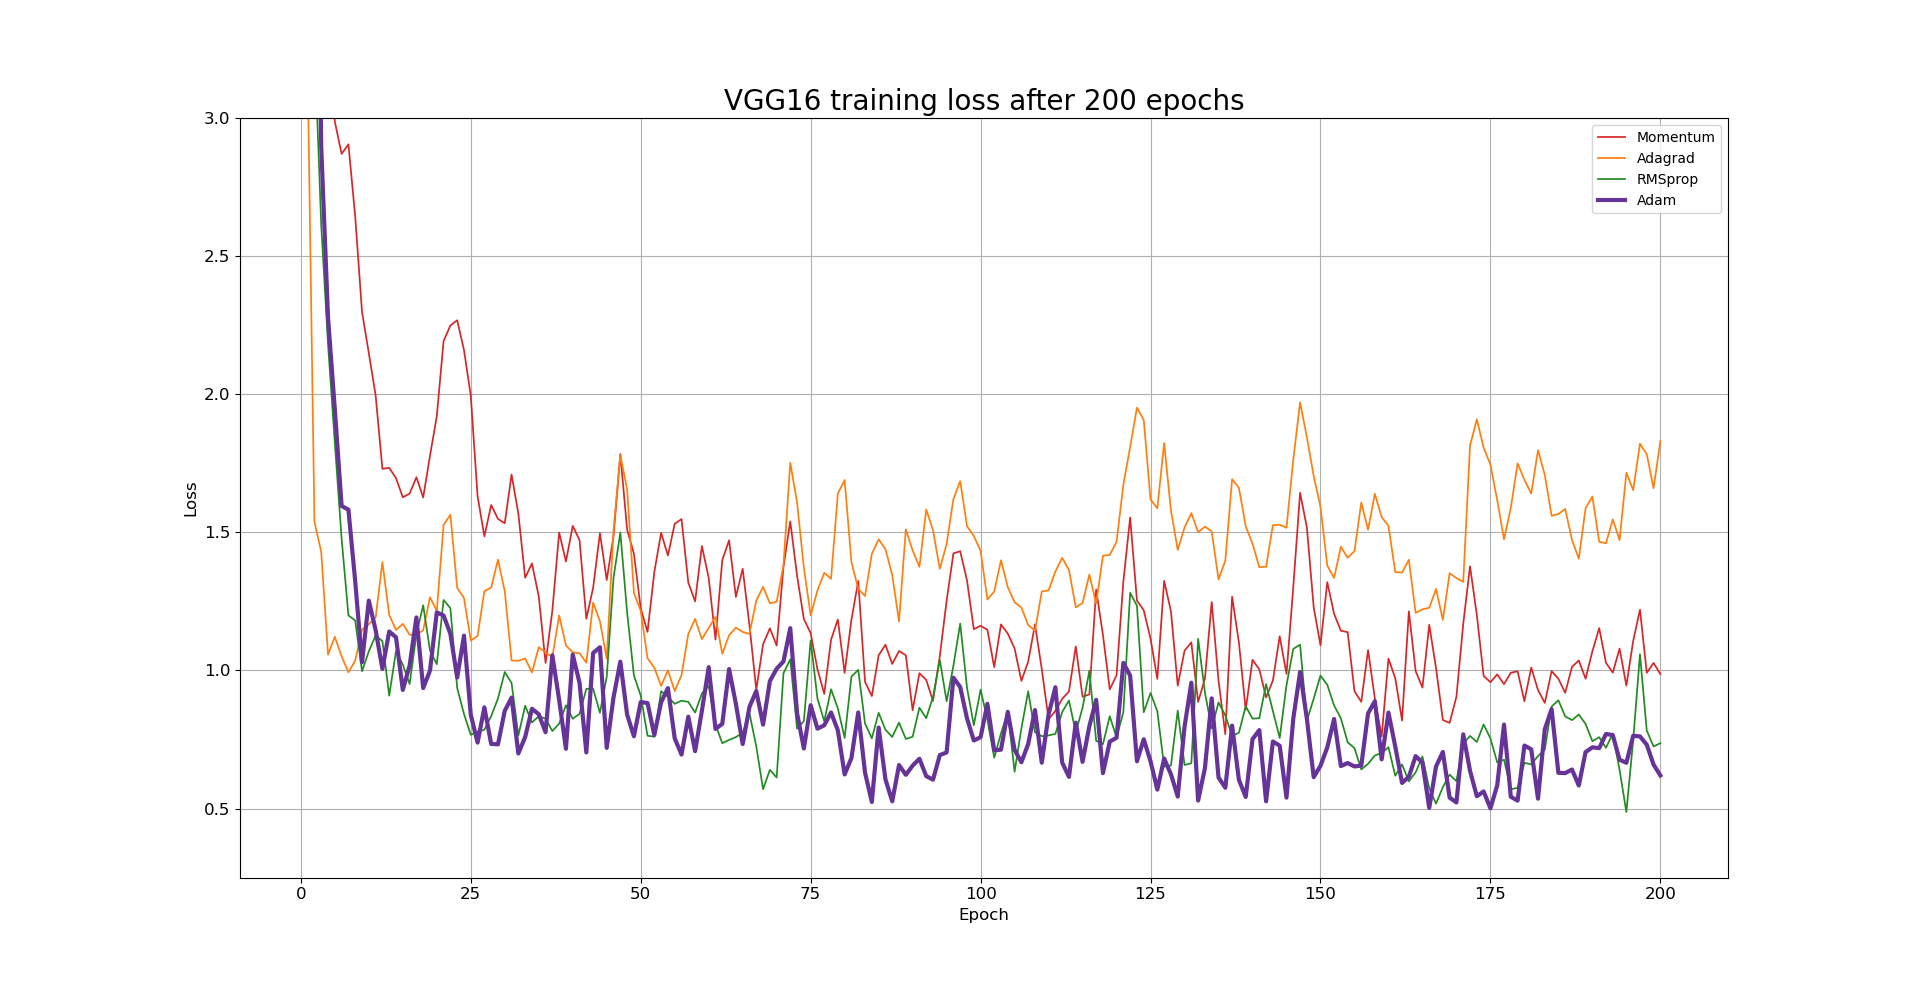
\includegraphics[width=140 mm]{images/vgg16.png}
	\caption{Đường đi của các thuật toán trong bề mặt lỗi (trái) và độ lỗi (phải) của từng thuật toán trong trường hợp đặc trưng thưa.}
	\label{fig:vgg16-loss}
\end{figure}

Quá trình huấn luyện mô hình VGG16 trên tập dữ liệu ImageNet (hình \ref{fig:vgg16-loss}) cho thấy Adam là thuật toán hiệu quả nhất trong số các thuật toán được thí nghiệm khi có độ lỗi giảm nhanh chóng và ổn định. Trái lại, Adagrad không những có độ dao động khá cao mà còn có xu hướng cho độ lỗi tăng trong những epoch cuối của quá trình huấn luyện, trở thành thuật toán có độ lỗi cao nhất. Thuật toán Momentum cho độ lỗi thấp thứ ba (sau RMSprop và Adam) nhưng sự chênh lệch độ lỗi giữa Momentum và Adam là rất lớn. Chỉ RMSprop là có độ lỗi gần với Adam nhất, nhưng RMSprop cũng có biên độ dao động lớn hơn.

\subsubsection{Huấn luyện mô hình ngôn ngữ}
\label{exp:lstm}

Chúng tôi sử dụng thiết lập giống trong bài báo của Zaremba và cộng sự \cite{zaremba2014recurrent} cho mô hình LSTM-medium. Sử dụng kiến trúc mạng RNN gồm 2 tầng Long short-term memory (LSTM), mỗi tầng có 650 nơ-ron với số bước unroll là 35. Chúng tôi khởi khởi tạo hai tầng ẩn này bằng giá trị 0 và sử dụng trạng thái ẩn cuối cùng của minibatch $t$ làm giá trị khởi tạo của trạng thái ẩn của minibatch t+1 với kích thước của một minibatch là 20.

Các giá trị trọng số trong mạng được khởi tạo theo phân phối đều trong khoảng [-0.05,0.05]. Với tỷ lệ dropout là 0.5 cho các liên kết không hồi quy, mô hình được huấn luyện trong 39 epoch với tỷ lệ học được tuning tốt nhất cho mỗi thuật toán tối ưu và được trình bày trong bảng \ref{tab:lstm-hparam}. Trong quá trình huấn luyện, sau epoch thứ 6 thì tỷ lệ học sẽ được nhân với $\frac{5}{6}$ sau mỗi epoch. Để hạn chế hiện tượng gradient bất ổn định, ta sử dụng ``gradient clipping'' - kĩ thuật giới hạn giá trị tuyệt đối của gradient - với giá trị giới hạn là 5.

\begin{figure}[htp]
	\centering
	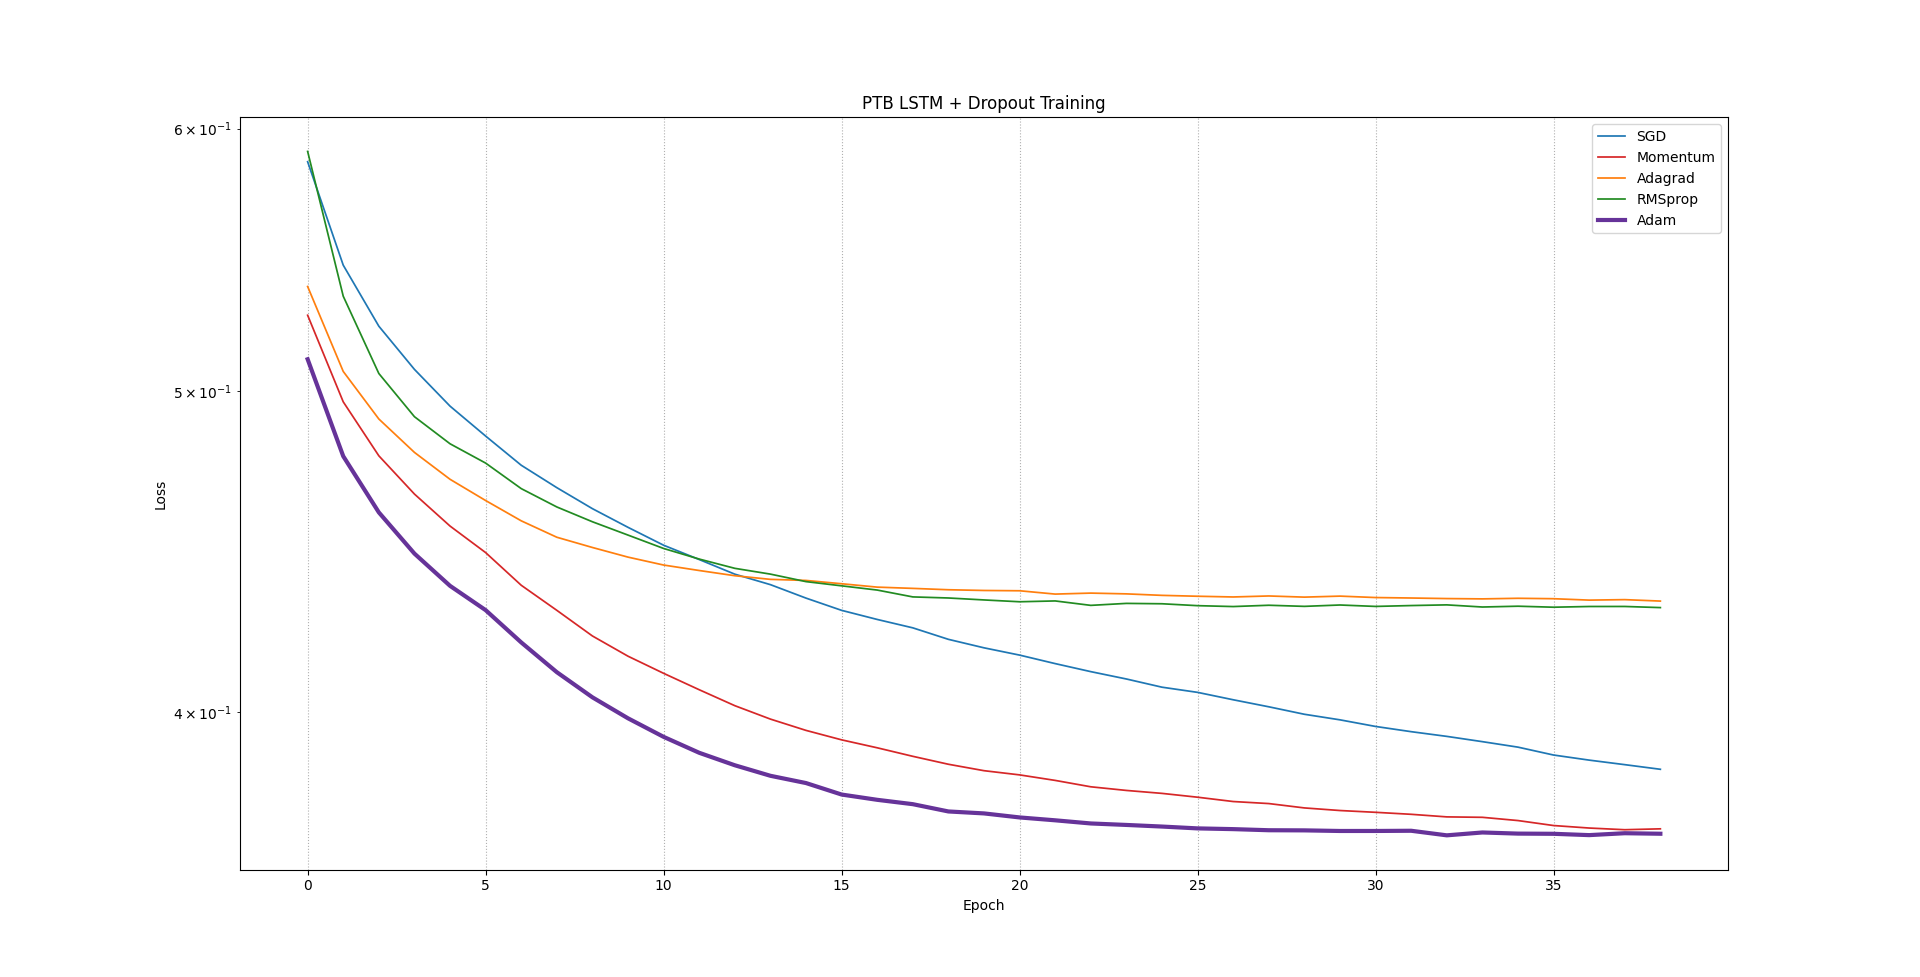
\includegraphics[width=140 mm]{images/ptb.png}
	\caption{Độ lỗi huấn luyện mô hình ngôn ngữ trên tập Penn TreeBank có sử dụng gradient clipping..}
	\label{fig:ptb}
\end{figure}

Hình \ref{fig:ptb} cho ta kết quả chạy của mô hình LSTM trên tập Penn Treebank trong 39 epoch. Nhìn chung Adam vẫn có độ lỗi nhỏ nhất và thời gian tiêu tốn ít nhất để tìm được đến độ lỗi này. Ta thấy được rằng Adam cho độ lỗi nhỏ nhất ngay từ những epoch đầu tiên, theo ngay sau đó là Momentum. Trong khi Adam vẫn còn tiếp tục di chuyển về vùng có độ lỗi nhỏ hơn, RMSprop và Adagrad đã bị chững lại tại điểm có độ lỗi khá cao. Thuật toán SGD vẫn tiếp tục đi xuống mặc dù tốc độ di chuyển chậm hơn Adam và Momentum. Có thể thấy rằng trong trường hợp trên, hai thuật toán SGD và Momentum cho độ lỗi thấp rất gần với Adam, trong đó Momentum đuổi kịp Adam tại những epoch cuối còn SGD mặc dù di chuyển chậm nhưng có xu hướng tiến gần hơn tới Adam và có thể đạt cùng độ lỗi với số lượng epoch lớn hơn. Giả thiết cho rằng việc giới hạn trung bình của gradient đã khiến cho trường hợp giá trị gradient rất khác nhau xảy ra rất ít, những vùng này là thế mạnh của các thuật toán Momentum và SGD giải thích lý do tại sao hai thuật toán này có thể bắt kịp với Adam.

\begin{figure}[htp]
	\centering
	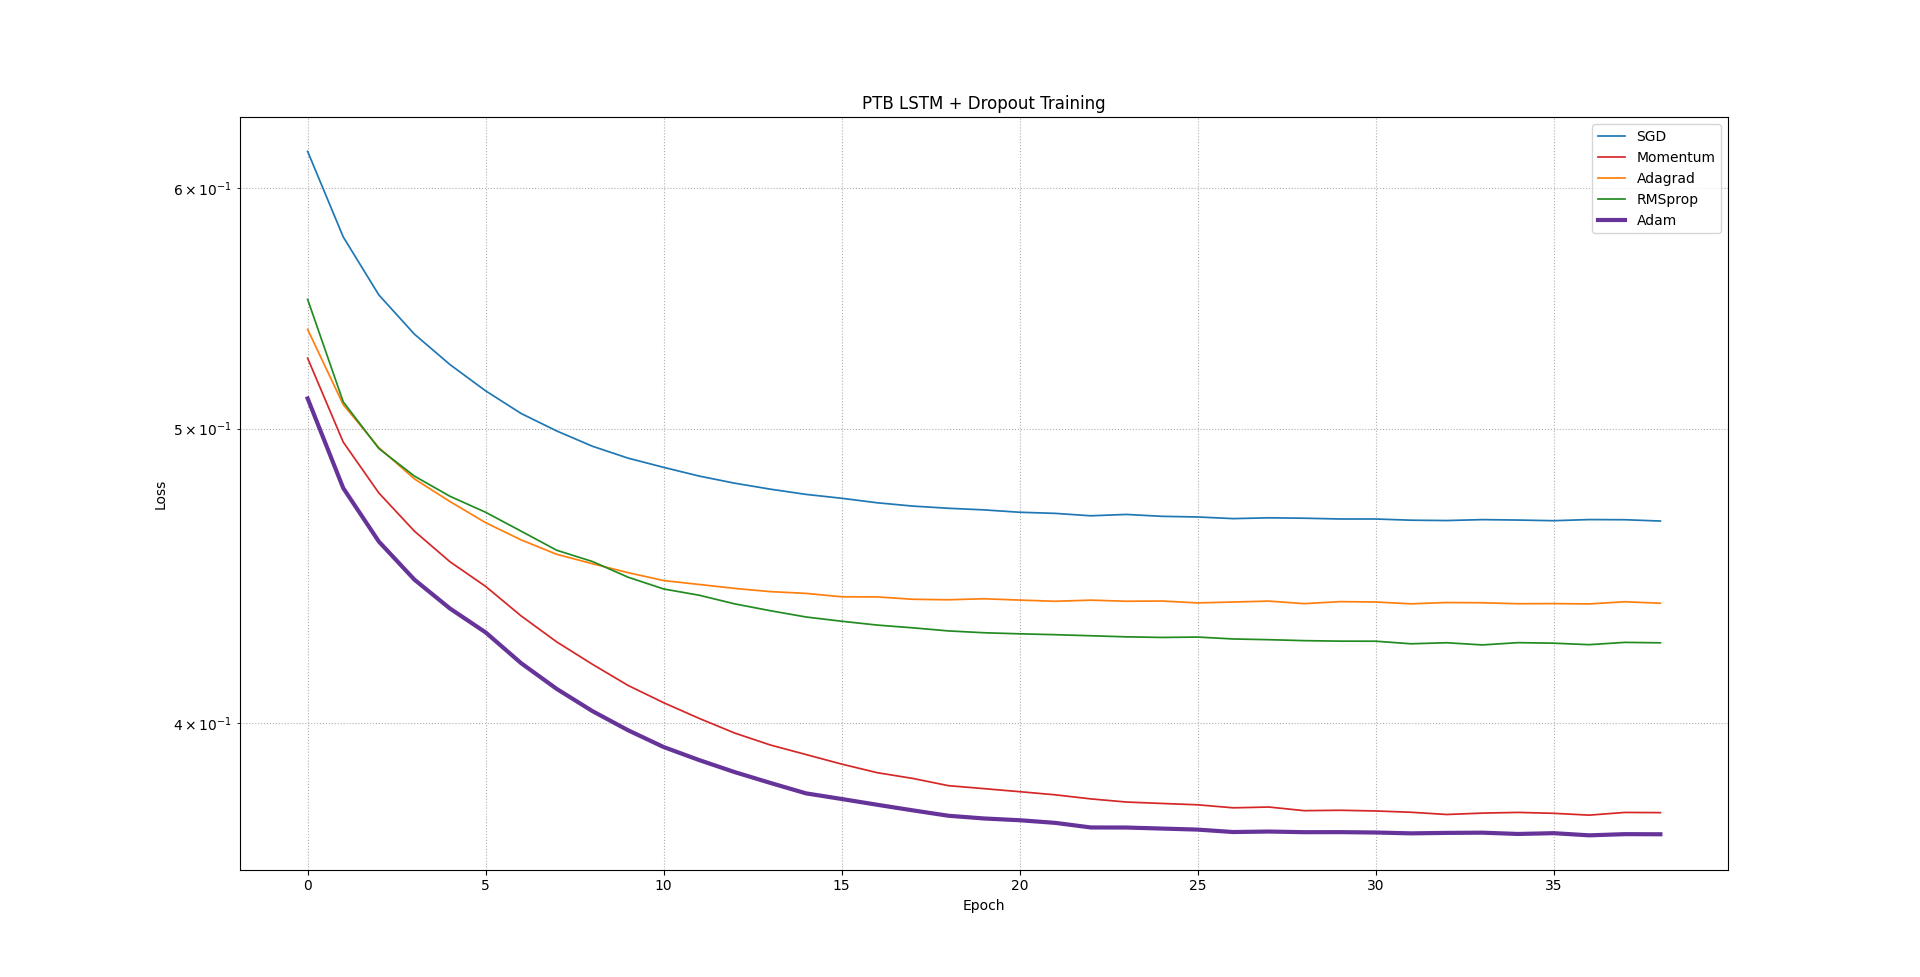
\includegraphics[width=140 mm]{images/ptb2.png}
	\caption{Độ lỗi huấn luyện mô hình ngôn ngữ trên tập dữ liệu Penn TreeBank không sử dụng gradient clipping.}
	\label{fig:ptb2}
\end{figure}

Hình \ref{fig:ptb2} là kết quả chạy của mô hình khi không giới hạn độ lớn của trung bình gradient. Nhìn tổng thể, ta có thể thấy Adam vẫn là thuật toán cho độ lỗi thấp nhất trong các thuật toán. Nếu ở trường hợp trước, SGD có thể gần như bắt kịp Adam thì ở đây SGD chững lại khá sớm và cho độ lỗi cao nhất trong năm thuật toán. Đây có thể là minh chứng cho giả thiết được đặt ra ở trường hợp trên. Ở đây bề mặt lỗi gồm nhiều vùng rãnh hẹp, các vùng này khiến SGD có độ lỗi giảm rất chậm tạo cảm giác thuật toán bị chững lại. Mặc dù Adagrad và RMSprop đã có sự cải thiện về mặt độ lỗi nhưng vẫn không thể tiến gần đến độ lỗi của Adam trước khi bị đi ngang. Nếu ở thí nghiệm trước, thuật toán Momentum gần như đuổi kịp Adam thì ở thí nghiệm này đã có một sự cách biệt giữa độ lỗi của hai thuật toán (từ 0,002 tăng lên 0,009). Thuật toán Adam vẫn cho độ lỗi trong tập huấn luyện là nhỏ nhất trong các thuật toán.

Các giá trị độ lỗi và thời gian chạy tương ứng với từng thuật toán được trình bày trong bảng \ref{tab:lstm-results}. Độ lỗi được thể hiện trong bảng bao gồm độ lỗi thấp nhất và cao nhất trong quá trình huấn luyện trên cả hai tập huấn luyện và tập kiểm thử.

\begin{table}
	\begin{adjustbox}{width=1\textwidth}
	\small
	\begin{tabular}{|l|>{\raggedright\arraybackslash}m{0.17\textwidth}|>{\raggedright\arraybackslash}m{0.14\textwidth}|>{\raggedright\arraybackslash}m{0.14\textwidth}|>{\raggedright\arraybackslash}m{0.125\textwidth}|>{\raggedright\arraybackslash}m{0.125\textwidth}|}
		\hline
		\textbf{Thuật toán} & \textbf{Thời gian thực hiện (giây)} & \textbf{Độ~lỗi huấn~luyện} & \textbf{Độ Perp. huấn~luyện} & \textbf{Độ~lỗi kiểm~thử} & \textbf{Độ Perp. kiểm~thử} \\
		\hline
		\multirow{2}{*}{SGD} & \textbf{21.78}        & 0.47 & 1.59 & 4.90 & 134.27 \\
							 & \textbf{$\pm$0.00023} & 0.62 & 1.85 & 6.39 & 593.27 \\
		\hline
		\multirow{2}{*}{Momentum} & \multirow{2}{*}{22.61$\pm$0.00025} & 0.37 & 1.45 & \textbf{4.40} & \textbf{81.82} \\
								  &                                    & 0.53 & 1.70 & \textbf{5.41} & \textbf{223.34} \\
		\hline
		\multirow{2}{*}{Adagrad} & \multirow{2}{*}{23.27$\pm$0.0054} & 0.44 & 1.54 & 4.71 & 110.94 \\
								 &                                   & 0.54 & 1.72 & 5.52 & 250.73 \\
		\hline
		\multirow{2}{*}{RMSprop} & \multirow{2}{*}{23.60$\pm$0.013} & 0.43 & 1.54 & 4.71 & 111.44 \\
								 &                                  & 0.59 & 1.80 & 6.00 & 402.50 \\
		\hline
		\multirow{2}{*}{Adam} & \multirow{2}{*}{26.21$\pm$0.46} & \textbf{0.37} & \textbf{1.44} & 4.47 & 87.78 \\
							  &                                 & \textbf{0.51} & \textbf{1.67} & 5.20 & 180.62 \\
		\hline
	\end{tabular}
	\end{adjustbox}
\caption{\label{tab:lstm-results}Kết quả và thời gian thực hiện một epoch của các thuật toán trong thí nghiệm Mô hình ngôn ngữ.}
\end{table}

Thông qua bảng dữ liệu \ref{tab:lstm-results}, ta thấy hiện tượng được Wilson và cộng sự đề cập trong bài báo \cite{wilson2017marginal}: mặc dù Adam cho độ lỗi nhỏ hơn Momentum trong tập huấn luyện nhưng lại cho kết quả độ lỗi ngoài tập huấn luyện cao hơn. Một số bài báo gần đây cố gắng đưa ra lời giải thích cho trường hợp thông qua lý thuyết về cực tiểu bằng phẳng (flat minima) thường nằm ở các vùng bằng phẳng hay tại đáy của các rãnh hẹp, ngược lại ta có cực tiểu nhọn (sharp minima). Dựa trên quan điểm các vùng cực tiểu bằng phẳng tổng quát hoá tốt hơn, Pan Zhou và cộng sự cho rằng lý do Adam có độ lỗi ngoài tập huấn luyện cao hơn SGD là do Adam dễ dàng hội tụ tại các vùng cực tiểu nhọn trong khi SGD lại có thể thoát khỏi vùng cực tiểu này để đến vùng cực tiểu bằng phẳng hơn \cite{zhou2020towards}. Tuy nhiên, vẫn có bài báo có quan điểm ngược lại, cho rằng: cực tiểu nhọn cho độ lỗi ngoài tập huấn luyện tốt hơn cực tiểu bằng \cite{li2018visualizing} nên đây vẫn chưa thể coi là lời giải thích chính thức cho hiện tượng này.

\chapter{Kết luận và hướng phát triển}
\label{Chapter5}

\section{Kết luận}

Trong khóa luận này, chúng tôi nghiên cứu về bài toán huấn luyện mạng nơ-ron nhiều tầng ẩn bằng thuật toán Adam. Cụ thể, chúng tôi tập trung tìm hiểu các khó khăn của việc huấn luyện một mạng nơ-ron nhiều tầng ẩn, cũng như cách mà các thuật toán tối ưu tiếp cận và giải quyết các khó khăn đó, với trọng tâm được đặt vào thuật toán Adam \cite{kingma2014adam}. Dưới đây là một số kết quả đạt được của khóa luận.

Chúng tôi tìm hiểu, cài đặt lại và sử dụng các thuật toán SGD, Momentum, Adagrad, RMSprop, Adam (cùng một số thuật toán khác) để kiểm tra cách hoạt động của các thuật toán này trong nhiều tình huống khác nhau, từ mô phỏng bằng dữ liệu ngẫu nhiên đến huấn luyện những kiến trúc mạng nơ-ron được sử dụng trong thực tế trên các tập dữ liệu phổ biến. Ngoài ra, chúng tôi cũng ứng dụng các phương pháp tăng tốc tính toán như véc-tơ hóa trên CPU (Central Processing Unit) bằng thư viện Numpy và tính toán song song trên GPU (Graphics Processing Unit) bằng thư viện Pytorch. Kết quả của các thuật toán do chúng tôi cài đặt có thể tái tạo được một phần kết quả được công bố trong bài báo. Ngoài ra, với kiến trúc VGG16 và tập dữ liệu ImageNet, chúng tôi sử dụng TPU (Tensor Processing Unit) trên nền tảng Google Cloud để rút ngắn thời gian thực hiện thí nghiệm.

Chúng tôi thực hiện một số thí nghiệm nhằm phân tích khả năng tối ưu của các thuật toán trong nhiều tình huống khác nhau. Chẳng hạn, chúng tôi phân tích cách mà các thuật toán di chuyển trong bề mặt rãnh hẹp, cụ thể là độ lớn của các bước cập nhật theo từng trục của rãnh. Ngoài ra, chúng tôi cũng xem xét các trường hợp tối ưu và không tối ưu của Adam. Kết quả cho thấy rằng Adam không chỉ phát huy được ưu điểm của các thuật toán cơ sở là Momentum và RMSprop về tốc độ và khả năng thích ứng tỉ lệ học, mà còn khắc phục được một số điểm yếu của các thuật toán này như sự dao động và khả năng sửa sai khi di chuyển lố qua khỏi điểm cực tiểu. Chúng tôi cũng thực hiện thí nghiệm trên các kiến trúc mạng nơ-ron nhiều tầng ẩn được sử dụng phổ biến hiện nay, và cho thấy rằng Adam thường đạt được kết quả tốt nhất.

Chúng tôi cũng phân tích một số hạn chế của thuật toán như:

\begin{itemize}
	\item Thời gian cần cho từng bước tối ưu của Adam lâu hơn các thuật toán còn lại do Adam thực hiện tính toán cả momentum lẫn thích ứng tỉ lệ học. Ngoài ra, Adam còn có thêm công đoạn bias-correction để các bước tối ưu đầu tiên không bị bias về 0. Tuy nhiên, sau khi đã thực hiện được nhiều bước cập nhật thì bước bias-correction này không còn cần thiết nữa. Vì vậy, về lâu dài, Adam vẫn tốn thời gian cho bước bias-correction nhưng lại không giúp ích cho quá trình cập nhật.
	\item Trong trường hợp rãnh hẹp có các trục không trùng với trọng số, Adam cũng gặp khó khăn như các thuật toán tỉ lệ học thích ứng khác. Các thuật toán này thực hiện thay đổi tỉ lệ học cho từng trọng số một cách riêng biệt, dẫn đến hiệu quả bị giảm sút khi rãnh hẹp có trục chéo, tức là có sự phụ thuộc giữa các trọng số với nhau.
\end{itemize}

\section{Hướng phát triển}

Placeholder

% Công trình của tác giả (nếu không có thì comment 02 dòng dưới)
%\addcontentsline{toc}{chapter}{Danh mục công trình của tác giả}
%\chapter*{Danh mục công trình của tác giả}
\label{Appendix1}

\begin{enumerate}
\item Tạp chí ABC
\item Tạp chí XYZ
\end{enumerate}

% In tài liệu tham khảo
\addcontentsline{toc}{chapter}{Tài liệu tham khảo}
\printbibheading[title={Tài liệu tham khảo}]

\printbibliography[heading=subbibliography, title={Tiếng Việt}, keyword=Viet, resetnumbers=true]

\DeclareNameAlias{sortname}{last-first}
\DeclareNameAlias{default}{last-first}

\printbibliography[heading=subbibliography, title={Tiếng Anh}, notkeyword=Viet, resetnumbers=4] 
% ===================================================================== %
% CHÚ Ý: phải gán lại resetnumbers=số tài liệu tham khảo tiếng Việt + 1 %
% ===================================================================== %

% Phần phụ lục
%s\appendix

\chapter{Các siêu tham số của các thí nghiệm}
\label{Appendix1}

\begin{table}[htp]
		\begin{tabularx}{\textwidth}{{|l|l|l|l|X|}}
			\hline
			\textbf{Thuật toán} & \textbf{Tỉ lệ học} & \textbf{Momentum/$\beta_1$} & \textbf{Alpha/$\beta_2$} & \textbf{$\epsilon$} \\
			\hline
			SGD               & 0.01   & -    & -     & -    \\
			\hline
			Momentum          & 0.01   & 0.9  & -     & -    \\
			\hline
			Adagrad           & 0.045  & -    & -     & 1e-8 \\
			\hline
			RMSprop           & 0.0001 & -    & 0.91  & 1e-8 \\
			\hline
			Adam              & 0.0001 & 0.91 & 0.998 & 1e-8 \\
			\hline
		\end{tabularx}
	\caption{\label{tab:mlp-hparam}Các siêu tham số được sử dụng trong thí nghiệm Multi-layer Neural Network.}
\end{table}

\begin{table}[htp]
	\begin{adjustbox}{width=1\textwidth}
	\small
	\begin{tabularx}{\textwidth}{{|l|l|l|l|l|X|}}
		\hline
		\textbf{Thuật toán} & \textbf{Mục đích} & \textbf{Tỉ lệ học} & \textbf{Momentum/$\beta_1$} & \textbf{Alpha/$\beta_2$} & \textbf{$\epsilon$} \\
		\hline
		SGD  & Tốt nhất & 0.1 & - & - & - \\
		\hline
		Momentum & Tốt nhất & 0.00728 & 0.9127 & - & - \\
		\hline
		Nesterov & Tái tạo & 0.001 & 0.99 & - & - \\
		\hline
		\multirow{2}{*}{Adagrad} & Tái tạo & 0.001 & - & - & - \\
				  				 & Tốt nhất & 0.01 & - & - & - \\
		\hline
		RMSprop & Tốt nhất & 0.0004338 & - & 0.9144 & 1e-8 \\
		\hline
		\multirow{2}{*}{Adam} & Tái tạo & 0.001 & 0.9 & 0.999965 & 1e-9 \\
		                      & Tốt nhất & 0.00033 & 0.5 & 0.999935 & 1e-8 \\
		\hline
	\end{tabularx}
	\end{adjustbox}
	\caption{\label{tab:cnn-hparam}Các siêu tham số được sử dụng trong thí nghiệm Convolutional Neural Network.}
\end{table}

\begin{table}[htp]
	\begin{tabularx}{\textwidth}{{|l|l|l|l|X|}}
		\hline
		\textbf{Thuật toán} & \textbf{Tỉ lệ học} & \textbf{Momentum/$\beta_1$} & \textbf{Alpha/$\beta_2$} & \textbf{$\epsilon$} \\
		\hline
		Momentum          & 1e-5 & 0.9  & -        & -    \\
		\hline
		Adagrad           & 1e-5 & -         & -        & 1e-8 \\
		\hline
		RMSprop           & 1e-6 & -         & 0.9     & 1e-8 \\
		\hline
		Adam              & 1e-6 & 0.9 & 0.999 & 1e-8 \\
		\hline
	\end{tabularx}
\caption{\label{tab:vgg16-hparam}Các siêu tham số được sử dụng trong thí nghiệm VGG16.}
\end{table}

\begin{table}[htp]
	\begin{tabularx}{\textwidth}{{|l|l|l|l|X|}}
		\hline
		\textbf{Thuật toán} & \textbf{Tỉ lệ học} & \textbf{Momentum/$\beta_1$} & \textbf{Alpha/$\beta_2$} & \textbf{$\epsilon$} \\
		\hline
		SGD               & 1        & -         & -        & -    \\
		\hline
		Momentum          & 0.666182 & 0.939152  & -        & -    \\
		\hline
		Adagrad           & 0.018393 & -         & -        & 1e-8 \\
		\hline
		RMSprop           & 0.003749 & -         & 0.91     & 1e-8 \\
		\hline
		Adam              & 0.001468 & 0.9277077 & 0.998469 & 1e-8 \\
		\hline
	\end{tabularx}
\caption{\label{tab:lstm-hparam}Các siêu tham số được sử dụng trong thí nghiệm mô hình ngôn ngữ.}
\end{table}
%\chapter{Tái tạo kết quả thí nghiệm Convolutional Neural Network}
\label{Appendix2}

Ngoài việc tìm bộ siêu tham số cho kết quả tốt nhất, chúng tôi cũng cố gắng tái tạo kết quả mà bài báo đã công bố. Chúng tôi thực hiện quá trình tái tạo này để kiểm tra tính khả thi của các kết quả mà bài báo đã công bố. Hình \ref{fig:exp-cnn-rep} là kết quả sát nhất với bài báo mà chúng tôi có thể tái tạo được từ khoảng tìm kiếm mà chúng tôi sử dụng. Có thể thấy được rằng, đường đi của các thuật toán trong hình \ref{fig:exp-cnn-best}a và \ref{fig:exp-cnn-rep} có dạng khá giống nhau. Mặc dù có thể tái tạo được hình dạng biểu đồ của các thuật toán, độ lỗi cuối cùng của các thuật toán trong hình \ref{fig:exp-cnn-rep} vẫn cao hơn so với kết quả tốt nhất mà chúng tôi ghi nhận được ở hình \ref{fig:exp-cnn-best}b.

\begin{figure}[htp]
	\centering
	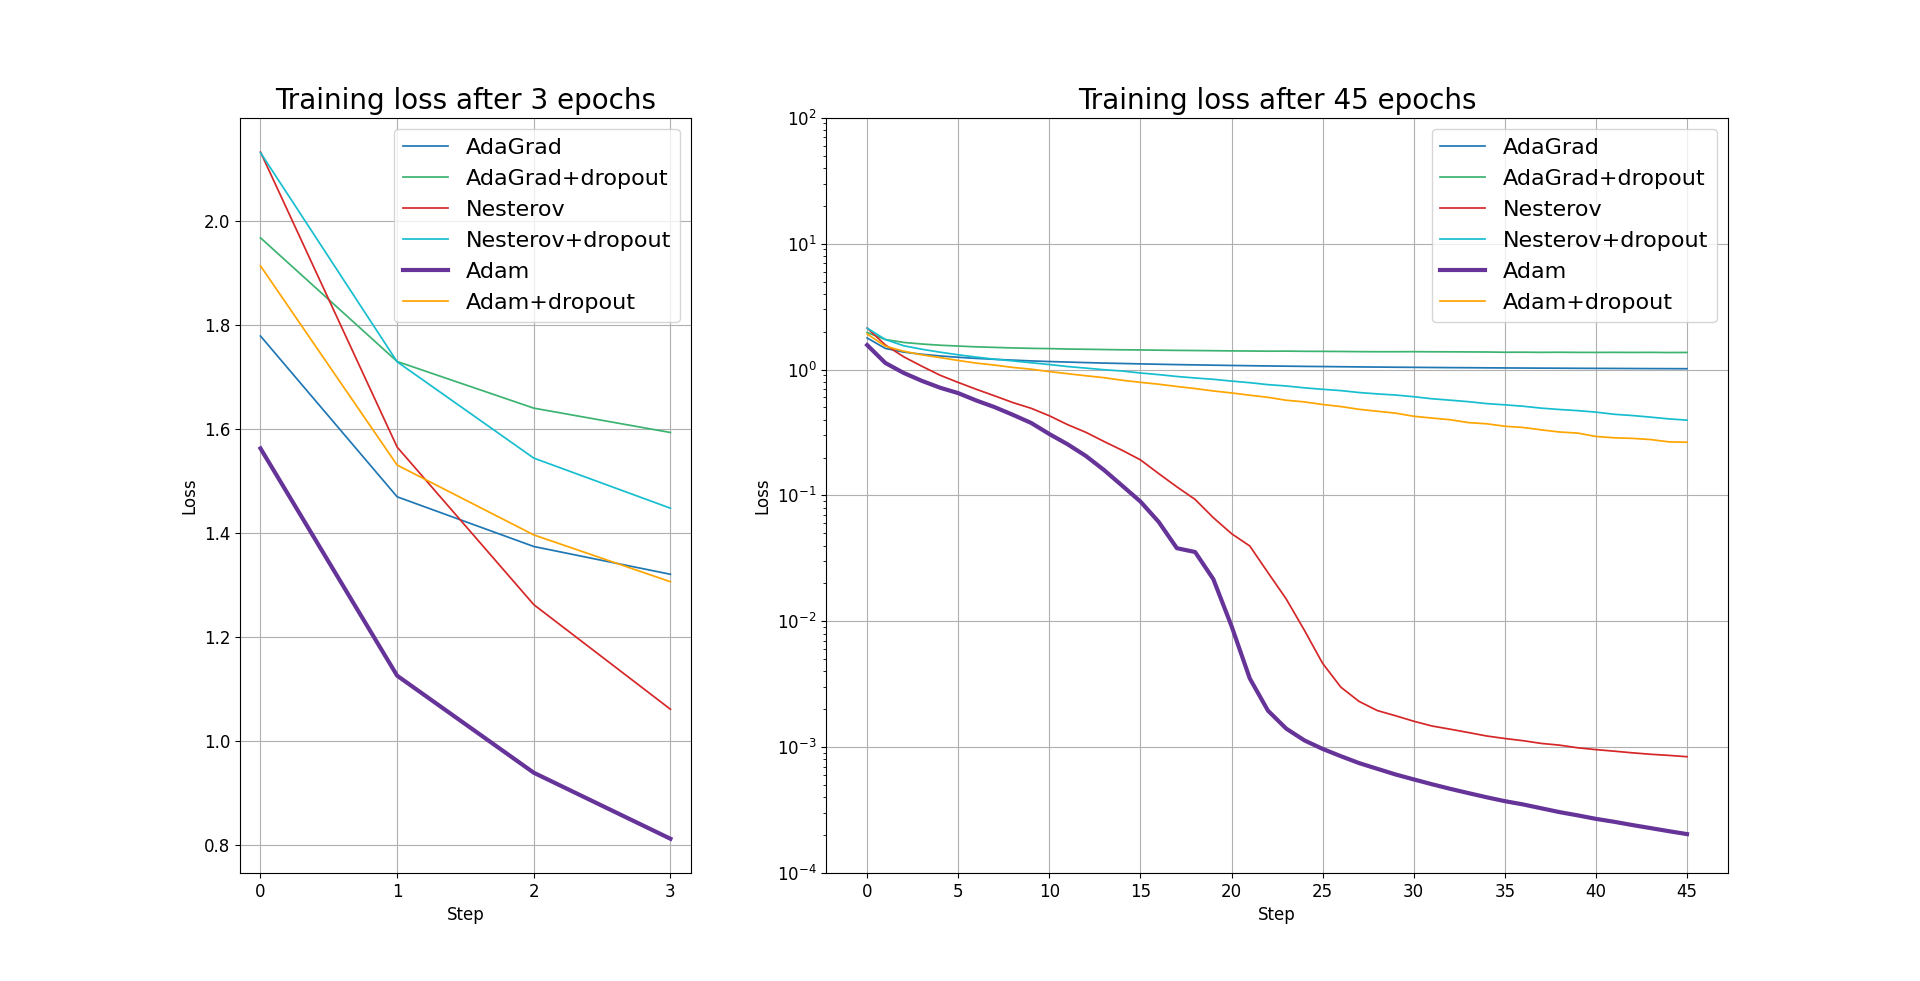
\includegraphics[width=140 mm]{images/cnn-rep.png}
	\caption{Kết quả thí nghiệm Convolutional Neural Network giữa thuật toán mà chúng tôi cài đặt với bộ siêu tham số mô phỏng kết quả của bài báo.}
	\label{fig:exp-cnn-rep}
\end{figure}

Ngoài lí do tác giả không công bố siêu tham số, cũng như tính chất ngẫu nhiên của SGD, một nguyên nhân khả thi khác cho sự khác biệt giữa kết quả mà chúng tôi ghi nhận được so với kết quả mà bài báo công bố là bản chất cài đặt của thư viện. Mỗi thư viện có cách xử lý tính toán riêng dẫn đến kết quả có phần lệch nhau. Vì tác giả cũng không nói rõ thư viện được sử dụng trong bài báo, nên thư viện Pytorch mà chúng tôi sử dụng có thể sẽ ra kết quả khác so với bài báo.

\end{document} 